% !TEX root = Users/ems/projects/macro3_project/paper/report.tex

\documentclass[a4paper]{article}

\usepackage[margin=1in]{geometry}
\usepackage{array}
\usepackage{hhline}
\usepackage[table]{xcolor}
\usepackage{threeparttable}
\usepackage{booktabs}
\usepackage{array}
\usepackage{longtable}
\usepackage{amsmath}
\usepackage{pdflscape}
\usepackage{graphicx}
\usepackage{xcolor}
% \definecolor{pagebg}{HTML}{fffff}
% \pagecolor{pagebg}


\newcolumntype{P}[1]{>{\raggedright\arraybackslash}p{#1}}

\newenvironment{centerbox}{\begin{center}}{\end{center}}

\providecommand{\huxb}[2]{\arrayrulecolor[RGB]{#1}\global\arrayrulewidth=#2pt}
\providecommand{\huxvb}[2]{\color[RGB]{#1}\vrule width #2pt}

\providecommand{\huxtpad}[1]{\rule{0pt}{2.2ex}}
\providecommand{\huxbpad}[1]{\rule[-0.8ex]{0pt}{0.8ex}}

\title{Macro Three Replication Project: Investigating the Economic Impact of the CFA Franc Zone with Synthetic Control Methods}
\date{Due: 29 May 2026}
\author{Callista Lodzinski, Mathilde Muller, and Elizabeth Schuck}

\begin{document}

\maketitle

Test

\section{Replication Target}
In this project, we aim to replicate the findings of \textit{From the French franc to the euro, is there an economic impact for the CFA franc zone countries? A 'bias-corrected' synthetic control method} by Alassane Diallo and Adama Ba, published in Cogent Economics \& Finance in 2024. This paper assesses the impact of pegging the CFA franc to the euro on real GDP per capita in the West African Economic and Monetary Union (WAEMU) and the Central African Economic and Monetary Community (CAEMC) countries. The original study uses a set of 35 annual country-level panel data from 1980 to 2019 and applies synthetic control methods to estimate the counterfactual economic outcomes for member countries.

%\input{} % Use \input{} to include the content of other .tex files (such as charts). E.g. \input{../output/tables/regression_table.tex}.


\section{Data}

\begin{table}[htbp]
\centering
\caption{Variables}
\begin{tabular}{llllll}
\hline
\textbf{Variable} &\textbf{Type} & \textbf{Category} & \textbf{(First) Page Ref} & \textbf{Possible Sources} \\
\hline

Real GDP per capita &  Continuous & Outcome & 6 & WDI, PennWorld Tables \\

Lagged GDP per capita & Continuous & Lagged outcome & 10 & WDI, PennWorld Tables \\

Gross Fixed Capital Formation (\% GDP) & Continuous & Capital & 10 &  \\

Government expenditure (\% GDP) & Continuous & Fiscal & 10 & WDI, PennWorld Tables \\

Official Development Assistance (\% GDP) & Continuous & External & 10 & Source not listed \\

Foreign Development Investment (\% GDP) & Continuous & External & 10 & WDI \\

Employment rate & Continuous & Labour & 10 & WDI \\

Agriculture (\% GDP) & Continuous & Structure & 10 & WDI, PennWorld Tables \\

Industry (\% GDP) &  Continuous & Structure & 10 & WDI, PennWorld Tables \\

Governance / institutional quality & Index & Institutions & 10 & Polity5 Dataset \\

Political regime characteristics & Categorical/Index & Institutions & 10 & Polity5 Dataset \\

Inflation &  Continuous & Macro controls & 5 & WDI, PennWorld Tables \\

\hline

Euro peg dummy & Binary & Treatment &  & Authors \\

\hline
\hline

Synthetic GDP per capita & $\tilde{Y}_{it}$ & Continuous & Constructed &  &  \\

Treatment effect & $\tau_{it}$ & Continuous & Constructed &  &  \\

\hline
\end{tabular}
\end{table}



% \begin{table}

\caption{CFA franc zone countries annual inflation rate: WAEMU}
\centering
\begin{tabular}[t]{lrr}
\toprule
country & 1980--2001 & 2002--2021\\
\midrule
Benin & 7.5270 & 2.1268\\
Burkina Faso & 4.3427 & 2.2660\\
Cote d'Ivoire & 8.5558 & 2.1842\\
Guinea-Bissau & 39.2343 & 2.8921\\
Mali & 8.6642 & 3.5490\\
\addlinespace
Niger & 6.0235 & 2.8630\\
Senegal & 5.1354 & 1.8448\\
Togo & 6.2716 & 2.0069\\
Average inflation for the WAEMU zone & 10.7193 & 2.4666\\
Average inflation without Guinea-Bissau & 6.6457 & 2.4058\\
\bottomrule
\end{tabular}
\end{table}
% \begin{table}

\caption{CFA franc zone countries annual inflation rate: CAEMC}
\centering
\begin{tabular}[t]{lrr}
\toprule
country & 1980--2001 & 2002--2021\\
\midrule
Cameroon & 7.0840 & 1.8268\\
Central African Republic & 6.5481 & 2.9430\\
Chad & 5.2621 & 5.4660\\
Congo, Rep. & 7.3655 & 6.1262\\
Equatorial Guinea & 11.0392 & 6.7586\\
\addlinespace
Gabon & 7.4425 & 3.7486\\
Average inflation for the CAEMC zone & 7.4569 & 4.4782\\
\bottomrule
\end{tabular}
\end{table}
% \begin{table}

\caption{Non-CFA franc zone countries mean annual inflation rate}
\centering
\begin{tabular}[t]{lrr}
\toprule
country & 1980--2001 & 2002--2021\\
\midrule
Angola & 961.3987 & 26.7149\\
Burundi & 10.9329 & 8.1400\\
Congo, Dem. Rep. & 1596.1468 & 10.5084\\
Ethiopia & 5.1686 & 14.6552\\
Gambia, The & 10.6514 & 6.7937\\
\addlinespace
Ghana & 37.8638 & 13.5181\\
Guinea & NaN & 14.8817\\
Kenya & 13.9999 & 8.7843\\
Madagascar & 17.2146 & 8.4518\\
Malawi & 24.4646 & 13.6236\\
\addlinespace
Nigeria & 24.5977 & 12.2867\\
Sao Tome and Principe & 24.0933 & 12.2127\\
Sierra Leone & NaN & 10.0007\\
Sudan & 53.8439 & 46.9048\\
Tanzania & 24.6668 & 6.8003\\
\addlinespace
Uganda & 5.3814 & 6.3894\\
Zambia & 67.9163 & 12.5346\\
Zimbabwe & NaN & 77.5202\\
Average inflation & 191.8894 & 17.2623\\
\bottomrule
\end{tabular}
\end{table}
% \begin{table}

\caption{WAEMU countries' mean annual GDP per capita growth: PWT and WDI GDP variables}
\centering
\begin{tabular}[t]{lrrrr}
\toprule
country & gdp\_pc 1990-2001 & gdp\_pc 2002-2021 & gdp\_pc\_wdi 1990-2001 & gdp\_pc\_wdi 2002-2021\\
\midrule
Benin & 2.3780 & 3.6640 & 3.589 & 3.5050\\
Burkina Faso & 2.1090 & 2.3180 & 4.832 & 4.9760\\
Cote d'Ivoire & -1.4560 & 4.6860 & 0.921 & 3.7480\\
Guinea-Bissau & 1.2690 & 0.8420 & 2.823 & 4.5390\\
Mali & 6.1440 & 3.2030 & 4.693 & 3.0080\\
\addlinespace
Niger & -0.6440 & 0.8010 & 0.873 & 3.4760\\
Senegal & -0.0920 & 0.8480 & 2.788 & 3.6670\\
Togo & -0.9470 & 4.5340 & 1.890 & 3.5730\\
Average for the WAEMU area & 1.0950 & 2.6120 & 2.801 & 3.8110\\
Average without Guinea-Bissau & 1.0703 & 2.8649 & 2.798 & 3.7076\\
\addlinespace
Average without Guinea-Bissau & 1.0703 & 2.8649 & 2.798 & 3.7076\\
\bottomrule
\end{tabular}
\end{table}
% \begin{table}

\caption{CAEMC countries' mean annual GDP per capita growth: PWT and WDI GDP variables}
\centering
\begin{tabular}[t]{lrrrr}
\toprule
country & gdp\_pc 1990-2001 & gdp\_pc 2002-2021 & gdp\_pc\_wdi 1990-2001 & gdp\_pc\_wdi 2002-2021\\
\midrule
Cameroon & -0.394 & 1.778 & -0.893 & 4.667\\
Central African Republic & -1.317 & 0.249 & -3.905 & 4.324\\
Chad & -0.920 & 3.472 & -0.840 & 10.432\\
Congo, Rep. & 2.000 & 5.218 & 0.293 & 7.294\\
Equatorial Guinea & 20.730 & 5.369 & 26.017 & 10.281\\
\addlinespace
Gabon & 0.710 & 3.720 & 0.111 & 4.900\\
Average for the CAEMC zone & 3.468 & 3.301 & 3.464 & 6.983\\
\bottomrule
\end{tabular}
\end{table}
% \begin{table}

\caption{Non-CFA countries' mean annual GDP per capita growth: PWT and WDI GDP variables}
\centering
\begin{tabular}[t]{lrrrr}
\toprule
country & gdp\_pc 1990-2001 & gdp\_pc 2002-2021 & gdp\_pc\_wdi 1990-2001 & gdp\_pc\_wdi 2002-2021\\
\midrule
Angola & -1.080 & 7.569 & -1.293 & 1.432\\
Burundi & -2.298 & 0.394 & -3.034 & 0.049\\
Congo, Dem. Rep. & -9.217 & 3.809 & -8.169 & 2.108\\
Ethiopia & -0.422 & 8.390 & 0.003 & 5.781\\
Gambia, The & 0.116 & -0.795 & 0.305 & 0.157\\
\addlinespace
Ghana & 0.871 & 3.227 & 1.746 & 3.462\\
Guinea & -2.300 & -0.454 & 1.252 & 2.247\\
Kenya & -0.277 & 3.831 & -0.895 & 1.768\\
Madagascar & -0.579 & 1.062 & -1.023 & -0.393\\
Malawi & -1.973 & 2.291 & 1.134 & 1.959\\
\addlinespace
Nigeria & 2.047 & 10.405 & -0.632 & 2.152\\
Sao Tome and Principe & 1.790 & 2.839 & 0.060 & 1.953\\
Sierra Leone & -1.305 & 3.146 & -3.661 & 2.642\\
Sudan & 1.158 & 3.806 & 3.862 & -0.546\\
Tanzania & 1.438 & 3.720 & 0.538 & 3.101\\
\addlinespace
Uganda & 3.577 & 2.640 & 3.166 & 2.919\\
Zambia & -0.045 & 5.263 & -0.514 & 2.231\\
Zimbabwe & -1.315 & 0.359 & 0.346 & -0.771\\
Average & -0.545 & 3.417 & -0.378 & 1.792\\
\bottomrule
\end{tabular}
\end{table}


% % \begin{table}

\caption{GDP method comparison for AGO}
\centering
\begin{tabular}[t]{llrrrrrr}
\toprule
country & method & 1980-2021 & 1990-2001 & 2002-2021 & n 1980-2021 & n 1990-2001 & n 2002-2021\\
\midrule
Angola & growth\_factor & 1.0244 & 0.9853 & 1.0717 & 39 & 12 & 18\\
Angola & index\_change\_from\_1990 & 40.6359 & -9.2907 & 91.5151 & 40 & 12 & 18\\
Angola & log\_growth & 1.6480 & -2.1830 & 6.0821 & 39 & 12 & 18\\
Angola & pct\_growth & 2.4407 & -1.4653 & 7.1684 & 39 & 12 & 18\\
Angola & growth\_factor & 1.0250 & 0.9865 & 1.0723 & 39 & 12 & 18\\
\addlinespace
Angola & index\_change\_from\_1990 & 41.5124 & -15.1002 & 99.3930 & 40 & 12 & 18\\
Angola & log\_growth & 1.6146 & -2.2800 & 6.0638 & 39 & 12 & 18\\
Angola & pct\_growth & 2.5030 & -1.3499 & 7.2327 & 39 & 12 & 18\\
Angola & growth\_factor & 1.0254 & 0.9889 & 1.0712 & 39 & 12 & 18\\
Angola & index\_change\_from\_1990 & 42.8099 & -6.8674 & 95.2394 & 40 & 12 & 18\\
\addlinespace
Angola & log\_growth & 1.7364 & -1.8919 & 6.0563 & 39 & 12 & 18\\
Angola & pct\_growth & 2.5383 & -1.1105 & 7.1167 & 39 & 12 & 18\\
Angola & growth\_factor & 1.0031 & 0.9848 & 1.0206 & 39 & 12 & 18\\
Angola & index\_change\_from\_1990 & 5.6979 & -18.6092 & 23.0705 & 40 & 12 & 18\\
Angola & log\_growth & 0.0686 & -2.0153 & 1.8884 & 39 & 12 & 18\\
\addlinespace
Angola & pct\_growth & 0.3120 & -1.5197 & 2.0564 & 39 & 12 & 18\\
Angola & growth\_factor & 1.0275 & 0.9892 & 1.0757 & 39 & 12 & 18\\
Angola & index\_change\_from\_1990 & 48.4202 & -11.9331 & 113.6706 & 40 & 12 & 18\\
Angola & log\_growth & 1.8587 & -1.7830 & 6.2262 & 39 & 12 & 18\\
Angola & pct\_growth & 2.7523 & -1.0796 & 7.5692 & 39 & 12 & 18\\
\addlinespace
Angola & growth\_factor & 0.9994 & 0.9826 & 1.0143 & 41 & 12 & 20\\
Angola & index\_change\_from\_1990 & 6.4294 & -18.7752 & 20.1983 & 42 & 12 & 20\\
Angola & log\_growth & -0.2871 & -2.2457 & 1.2887 & 41 & 12 & 20\\
Angola & pct\_growth & -0.0573 & -1.7407 & 1.4317 & 41 & 12 & 20\\
Angola & growth\_factor & 1.0591 & 0.9813 & 1.1195 & 41 & 12 & 20\\
\addlinespace
Angola & index\_change\_from\_1990 & 93.6779 & -42.3873 & 234.5528 & 42 & 12 & 20\\
Angola & log\_growth & 2.8062 & -4.4279 & 7.3137 & 41 & 12 & 20\\
Angola & pct\_growth & 5.9118 & -1.8725 & 11.9469 & 41 & 12 & 20\\
Angola & growth\_factor & 1.0047 & 0.9871 & 1.0143 & 31 & 11 & 20\\
Angola & index\_change\_from\_1990 & 5.5832 & -18.7752 & 20.1983 & 32 & 12 & 20\\
\addlinespace
Angola & log\_growth & 0.1848 & -1.8222 & 1.2887 & 31 & 11 & 20\\
Angola & pct\_growth & 0.4650 & -1.2926 & 1.4317 & 31 & 11 & 20\\
Angola & growth\_factor & 1.0320 & 1.0075 & 1.0455 & 31 & 11 & 20\\
Angola & index\_change\_from\_1990 & 55.9656 & -8.3014 & 94.5257 & 32 & 12 & 20\\
Angola & log\_growth & 2.8134 & 0.2344 & 4.2319 & 31 & 11 & 20\\
\addlinespace
Angola & pct\_growth & 3.1977 & 0.7450 & 4.5467 & 31 & 11 & 20\\
Angola & growth\_factor & 1.0026 & 0.9832 & 1.0221 & 39 & 12 & 18\\
Angola & index\_change\_from\_1990 & 7.6052 & -18.5389 & 24.2830 & 40 & 12 & 18\\
Angola & log\_growth & 0.0245 & -2.1851 & 2.0646 & 39 & 12 & 18\\
Angola & pct\_growth & 0.2609 & -1.6759 & 2.2099 & 39 & 12 & 18\\
\addlinespace
Angola & growth\_factor & 1.0629 & 0.9819 & 1.1337 & 39 & 12 & 18\\
Angola & index\_change\_from\_1990 & 96.2219 & -42.2383 & 255.8208 & 40 & 12 & 18\\
Angola & log\_growth & 3.2616 & -4.3673 & 8.7268 & 39 & 12 & 18\\
Angola & pct\_growth & 6.2931 & -1.8057 & 13.3653 & 39 & 12 & 18\\
Angola & growth\_factor & 1.0091 & 0.9878 & 1.0221 & 29 & 11 & 18\\
\addlinespace
Angola & index\_change\_from\_1990 & 7.1542 & -18.5389 & 24.2830 & 30 & 12 & 18\\
Angola & log\_growth & 0.6149 & -1.7574 & 2.0646 & 29 & 11 & 18\\
Angola & pct\_growth & 0.9077 & -1.2231 & 2.2099 & 29 & 11 & 18\\
Angola & growth\_factor & 1.0339 & 1.0082 & 1.0497 & 29 & 11 & 18\\
Angola & index\_change\_from\_1990 & 53.9862 & -8.0177 & 95.3222 & 30 & 12 & 18\\
\addlinespace
Angola & log\_growth & 3.0173 & 0.2992 & 4.6784 & 29 & 11 & 18\\
Angola & pct\_growth & 3.3927 & 0.8158 & 4.9676 & 29 & 11 & 18\\
Angola & direct & -0.0573 & -1.7407 & 1.4317 & 41 & 12 & 20\\
\bottomrule
\end{tabular}
\end{table}
% % \begin{table}

\caption{GDP method comparison for BEN}
\centering
\begin{tabular}[t]{llrrrrrr}
\toprule
country & method & 1980-2021 & 1990-2001 & 2002-2021 & n 1980-2021 & n 1990-2001 & n 2002-2021\\
\midrule
Benin & growth\_factor & 1.0149 & 1.0214 & 1.0376 & 39 & 12 & 18\\
Benin & index\_change\_from\_1990 & 43.8532 & 5.3929 & 79.1517 & 40 & 12 & 18\\
Benin & log\_growth & 1.2244 & 2.0054 & 3.6223 & 39 & 12 & 18\\
Benin & pct\_growth & 1.4889 & 2.1420 & 3.7590 & 39 & 12 & 18\\
Benin & growth\_factor & 1.0154 & 1.0238 & 1.0366 & 39 & 12 & 18\\
\addlinespace
Benin & index\_change\_from\_1990 & 48.2725 & 6.4867 & 83.8784 & 40 & 12 & 18\\
Benin & log\_growth & 1.1674 & 2.2417 & 3.5315 & 39 & 12 & 18\\
Benin & pct\_growth & 1.5423 & 2.3778 & 3.6636 & 39 & 12 & 18\\
Benin & growth\_factor & 1.0142 & 1.0215 & 1.0369 & 39 & 12 & 18\\
Benin & index\_change\_from\_1990 & 44.3284 & 6.0907 & 78.3218 & 40 & 12 & 18\\
\addlinespace
Benin & log\_growth & 1.1555 & 2.0165 & 3.5513 & 39 & 12 & 18\\
Benin & pct\_growth & 1.4248 & 2.1515 & 3.6907 & 39 & 12 & 18\\
Benin & growth\_factor & 1.0234 & 1.0207 & 1.0346 & 39 & 12 & 18\\
Benin & index\_change\_from\_1990 & 26.9422 & 8.2695 & 55.4429 & 40 & 12 & 18\\
Benin & log\_growth & 2.2432 & 2.0303 & 3.3362 & 39 & 12 & 18\\
\addlinespace
Benin & pct\_growth & 2.3379 & 2.0736 & 3.4587 & 39 & 12 & 18\\
Benin & growth\_factor & 1.0136 & 1.0235 & 1.0352 & 39 & 12 & 18\\
Benin & index\_change\_from\_1990 & 48.3190 & 6.6976 & 81.2933 & 40 & 12 & 18\\
Benin & log\_growth & 0.9802 & 2.2079 & 3.3902 & 39 & 12 & 18\\
Benin & pct\_growth & 1.3648 & 2.3455 & 3.5206 & 39 & 12 & 18\\
\addlinespace
Benin & growth\_factor & 1.0120 & 1.0183 & 1.0148 & 41 & 12 & 20\\
Benin & index\_change\_from\_1990 & 16.7945 & 6.4319 & 30.9259 & 42 & 12 & 20\\
Benin & log\_growth & 1.1521 & 1.7970 & 1.4522 & 41 & 12 & 20\\
Benin & pct\_growth & 1.1984 & 1.8291 & 1.4789 & 41 & 12 & 20\\
Benin & growth\_factor & 1.0425 & 1.0665 & 1.0540 & 41 & 12 & 20\\
\addlinespace
Benin & index\_change\_from\_1990 & 76.2245 & 3.6541 & 168.3044 & 42 & 12 & 20\\
Benin & log\_growth & 3.1801 & 4.3169 & 4.9254 & 41 & 12 & 20\\
Benin & pct\_growth & 4.2485 & 6.6491 & 5.3989 & 41 & 12 & 20\\
Benin & growth\_factor & 1.0148 & 1.0148 & 1.0148 & 31 & 11 & 20\\
Benin & index\_change\_from\_1990 & 21.7406 & 6.4319 & 30.9259 & 32 & 12 & 20\\
\addlinespace
Benin & log\_growth & 1.4543 & 1.4582 & 1.4522 & 31 & 11 & 20\\
Benin & pct\_growth & 1.4790 & 1.4792 & 1.4789 & 31 & 11 & 20\\
Benin & growth\_factor & 1.0353 & 1.0359 & 1.0350 & 31 & 11 & 20\\
Benin & index\_change\_from\_1990 & 75.4385 & 20.9266 & 108.1456 & 32 & 12 & 20\\
Benin & log\_growth & 3.4575 & 3.5148 & 3.4259 & 31 & 11 & 20\\
\addlinespace
Benin & pct\_growth & 3.5346 & 3.5885 & 3.5050 & 31 & 11 & 20\\
Benin & growth\_factor & 1.0117 & 1.0174 & 1.0147 & 39 & 12 & 18\\
Benin & index\_change\_from\_1990 & 15.0349 & 5.8072 & 29.0447 & 40 & 12 & 18\\
Benin & log\_growth & 1.1259 & 1.7145 & 1.4489 & 39 & 12 & 18\\
Benin & pct\_growth & 1.1717 & 1.7435 & 1.4744 & 39 & 12 & 18\\
\addlinespace
Benin & growth\_factor & 1.0411 & 1.0655 & 1.0525 & 39 & 12 & 18\\
Benin & index\_change\_from\_1990 & 68.5427 & 3.0203 & 161.9228 & 40 & 12 & 18\\
Benin & log\_growth & 3.0031 & 4.2344 & 4.7561 & 39 & 12 & 18\\
Benin & pct\_growth & 4.1083 & 6.5550 & 5.2511 & 39 & 12 & 18\\
Benin & growth\_factor & 1.0145 & 1.0140 & 1.0147 & 29 & 11 & 18\\
\addlinespace
Benin & index\_change\_from\_1990 & 19.7497 & 5.8072 & 29.0447 & 30 & 12 & 18\\
Benin & log\_growth & 1.4240 & 1.3831 & 1.4489 & 29 & 11 & 18\\
Benin & pct\_growth & 1.4467 & 1.4013 & 1.4744 & 29 & 11 & 18\\
Benin & growth\_factor & 1.0350 & 1.0351 & 1.0349 & 29 & 11 & 18\\
Benin & index\_change\_from\_1990 & 68.6953 & 20.1897 & 101.0324 & 30 & 12 & 18\\
\addlinespace
Benin & log\_growth & 3.4235 & 3.4397 & 3.4137 & 29 & 11 & 18\\
Benin & pct\_growth & 3.4979 & 3.5088 & 3.4912 & 29 & 11 & 18\\
Benin & direct & 1.2623 & 1.8291 & 1.4789 & 42 & 12 & 20\\
\bottomrule
\end{tabular}
\end{table}


% % \input{../output/gdp_exploration/countries/country_method_table_CMR.tex}
% % \input{../output/gdp_exploration/tables/table_pwt_pwt_cgdpo_pc_log_growth.tex}


% \begin{table}

\caption{Estimated synthetic control weights by treated country}
\centering
\begin{tabular}[t]{llllllllllllll}
\toprule
Donor country & Benin & Burkina Faso & Côte d'Ivoire & Mali & Niger & Senegal & Togo & Cameroon & Central African Republic & Chad & Republic of Congo & Gabon & Equatorial Guinea\\
\midrule
Bangladesh & .933 & 1.000 & .624 & .603 & .993 & .772 & .639 & .004 & 1.000 & .998 & .010 & 0 & 0\\
Barbados & .002 & 0 & 0 & 0 & 0 & .001 & 0 & 0 & 0 & .002 & 0 & 0 & 0\\
Bhutan & .001 & 0 & 0 & .020 & 0 & .005 & 0 & .035 & 0 & 0 & .248 & .039 & 0\\
Bolivia & 0 & 0 & .058 & .001 & 0 & .045 & 0 & 0 & 0 & 0 & 0 & 0 & 0\\
Botswana & .001 & 0 & 0 & 0 & 0 & .002 & 0 & 0 & 0 & 0 & .019 & 0 & 0\\
\addlinespace
Cabo Verde & 0 & 0 & 0 & 0 & 0 & .001 & 0 & 0 & 0 & 0 & 0 & 0 & .908\\
Dominica & .001 & 0 & .001 & 0 & 0 & .002 & 0 & 0 & 0 & 0 & .001 & 0 & 0\\
Ecuador & .001 & 0 & 0 & 0 & 0 & .004 & 0 & 0 & 0 & 0 & .255 & 0 & 0\\
Eswatini & 0 & 0 & .087 & 0 & 0 & .003 & 0 & 0 & 0 & 0 & .001 & .001 & 0\\
Grenada & .001 & 0 & 0 & 0 & 0 & .001 & 0 & 0 & 0 & 0 & .001 & 0 & 0\\
\addlinespace
Lao PDR & .049 & 0 & .002 & .086 & 0 & 0 & 0 & .333 & 0 & 0 & 0 & 0 & 0\\
Lesotho & 0 & 0 & .011 & .250 & .006 & .064 & .293 & .388 & 0 & 0 & .245 & .098 & 0\\
Mauritius & .001 & 0 & 0 & 0 & 0 & .001 & 0 & 0 & 0 & 0 & .001 & 0 & 0\\
Morocco & 0 & 0 & .004 & 0 & 0 & .003 & 0 & 0 & 0 & 0 & .003 & 0 & 0\\
Namibia & 0 & 0 & .001 & .001 & 0 & .004 & 0 & 0 & 0 & 0 & 0 & .439 & 0\\
\addlinespace
Oman & .001 & 0 & 0 & 0 & 0 & .001 & 0 & 0 & 0 & 0 & .001 & .245 & 0\\
Panama & .001 & 0 & 0 & 0 & 0 & .002 & 0 & 0 & 0 & 0 & 0 & 0 & 0\\
St. Kitts and Nevis & .001 & 0 & 0 & 0 & 0 & .001 & 0 & 0 & 0 & 0 & 0 & 0 & .038\\
St. Lucia & .001 & 0 & 0 & 0 & 0 & .001 & 0 & 0 & 0 & 0 & .003 & 0 & 0\\
Seychelles & .001 & 0 & 0 & 0 & 0 & .001 & 0 & 0 & 0 & 0 & .001 & 0 & 0\\
\addlinespace
Brunei & .003 & 0 & .016 & 0 & 0 & .002 & 0 & 0 & 0 & 0 & 0 & .063 & 0\\
Macao & 0 & 0 & 0 & 0 & 0 & 0 & 0 & 0 & 0 & 0 & 0 & 0 & 0\\
Libya & 0 & 0 & 0 & 0 & 0 & 0 & 0 & 0 & 0 & 0 & 0 & 0 & 0\\
Turkmenistan & 0 & 0 & .176 & .037 & 0 & .073 & .066 & .239 & 0 & 0 & .209 & .115 & 0\\
Eritrea & 0 & 0 & 0 & 0 & 0 & 0 & 0 & 0 & 0 & 0 & 0 & 0 & 0\\
\addlinespace
Guyana & 0 & 0 & 0 & 0 & 0 & .002 & 0 & 0 & 0 & 0 & 0 & 0 & 0\\
Iraq & .001 & 0 & 0 & 0 & 0 & .001 & 0 & 0 & 0 & 0 & 0 & 0 & .053\\
Qatar & 0 & 0 & 0 & 0 & 0 & 0 & 0 & 0 & 0 & 0 & 0 & 0 & 0\\
Djibouti & 0 & 0 & 0 & 0 & 0 & 0 & 0 & 0 & 0 & 0 & 0 & 0 & 0\\
El Salvador & .001 & 0 & .017 & .001 & 0 & .007 & 0 & 0 & 0 & 0 & 0 & 0 & 0\\
\bottomrule
\end{tabular}
\end{table}
% \begin{table}

\caption{The average of the predictors of per-capita GDP for franc-CFA zone countries}
\centering
\begin{tabular}[t]{lrrrrrr}
\toprule
country & avg\_agriculture & avg\_government & avg\_oda & avg\_fdi & avg\_labour & avg\_institution\\
\midrule
Benin & 29.961610 & 0.1633115 & 54778167 & 0.4055924 & 35.62389 & 2.925000\\
Synthetic Benin & 22.478334 & 0.1070643 & 345410573 & 0.4421463 & 32.94122 & 0.642225\\
Burkina Faso & 27.009303 & 0.1292807 & 137699348 & 0.6938516 & 40.17606 & -2.325000\\
Synthetic Burkina Faso & 24.760910 & 0.1176738 & 304775784 & 0.9008702 & 35.76767 & -0.301000\\
Côte d'Ivoire & 21.244944 & 0.1547087 & 58697793 & 1.1245368 & 31.40414 & -2.600000\\
\addlinespace
Synthetic Côte d'Ivoire & 20.151653 & 0.1447075 & 242361653 & 1.4067112 & 36.88903 & 1.995425\\
Mali & 31.924485 & 0.2248145 & 130880367 & 1.4313488 & 30.88820 & 1.650000\\
Synthetic Mali & 29.549045 & 0.1666256 & 152157580 & 2.2114470 & 42.45015 & -4.184825\\
Niger & 36.071288 & 0.2076225 & 133696937 & 2.2883942 & 41.15699 & 1.125000\\
Synthetic Niger & 23.187806 & 0.1015910 & 354917288 & 0.4702905 & 33.57220 & 0.975000\\
\addlinespace
Senegal & 16.892927 & 0.1675746 & 72103592 & 1.3178785 & 33.58079 & 3.150000\\
Synthetic Senegal & 21.627890 & 0.1699562 & 174787620 & 2.0670496 & 39.25406 & 0.107150\\
Togo & 21.379832 & 0.1584141 & 31225374 & 1.4919279 & 40.15292 & -3.775000\\
Synthetic Togo & 22.402575 & 0.1079749 & 343437691 & 0.4525850 & 32.90651 & 0.593175\\
Cameroon & 19.749879 & 0.1512596 & 53866423 & 1.2173302 & 39.96706 & -5.600000\\
\addlinespace
Synthetic Cameroon & 17.593541 & 0.1563369 & 227231922 & 1.0073854 & 32.31370 & 0.439050\\
Central African Republic & 37.435338 & 0.1980131 & 55865711 & 0.8982344 & 39.26813 & -0.625000\\
Synthetic Central African Republic & 23.187806 & 0.1015910 & 354917288 & 0.4702905 & 33.57220 & 0.975000\\
Chad & 34.548047 & 0.0753845 & 72635846 & 4.1151560 & 38.32956 & -1.850000\\
Synthetic Chad & 23.187806 & 0.1015910 & 354917288 & 0.4702905 & 33.57220 & 0.975000\\
\addlinespace
Republic of Congo & 7.863290 & 0.3325782 & 14367386 & 5.8508828 & 33.37802 & -4.125000\\
Synthetic Republic of Congo & 29.058136 & 0.2165515 & 32494584 & 3.1114775 & 45.95521 & -5.469375\\
Gabon & 6.291786 & 0.1734423 & 1457547 & 2.4415752 & 30.06796 & -3.375000\\
Synthetic Gabon & 14.442791 & 0.3083905 & 2748138 & 4.8687889 & 44.16803 & -2.879300\\
Equatorial Guinea & 6.788717 & 0.3130109 & 7265594 & 17.4621540 & 33.56924 & -6.250000\\
\addlinespace
Synthetic Equatorial Guinea & 8.145281 & 0.2086357 & 16934475 & 3.2506111 & 33.97505 & 5.693750\\
\bottomrule
\end{tabular}
\end{table}

% \begin{table}

\caption{The average of the predictors of per-capita GDP for franc-CFA zone countries}
\centering
\begin{tabular}[t]{lrrrrrr}
\toprule
country & avg\_agriculture & avg\_government & avg\_oda & avg\_fdi & avg\_labour & avg\_institution\\
\midrule
Benin & 29.961610 & 0.1633115 & 54778167 & 0.4055924 & 35.62389 & 2.925000\\
Synthetic Benin & 22.478334 & 0.1070643 & 345410573 & 0.4421463 & 32.94122 & 0.642225\\
Burkina Faso & 27.009303 & 0.1292807 & 137699348 & 0.6938516 & 40.17606 & -2.325000\\
Synthetic Burkina Faso & 24.760910 & 0.1176738 & 304775784 & 0.9008702 & 35.76767 & -0.301000\\
Côte d'Ivoire & 21.244944 & 0.1547087 & 58697793 & 1.1245368 & 31.40414 & -2.600000\\
\addlinespace
Synthetic Côte d'Ivoire & 20.151653 & 0.1447075 & 242361653 & 1.4067112 & 36.88903 & 1.995425\\
Mali & 31.924485 & 0.2248145 & 130880367 & 1.4313488 & 30.88820 & 1.650000\\
Synthetic Mali & 29.549045 & 0.1666256 & 152157580 & 2.2114470 & 42.45015 & -4.184825\\
Niger & 36.071288 & 0.2076225 & 133696937 & 2.2883942 & 41.15699 & 1.125000\\
Synthetic Niger & 23.187806 & 0.1015910 & 354917288 & 0.4702905 & 33.57220 & 0.975000\\
\addlinespace
Senegal & 16.892927 & 0.1675746 & 72103592 & 1.3178785 & 33.58079 & 3.150000\\
Synthetic Senegal & 21.627890 & 0.1699562 & 174787620 & 2.0670496 & 39.25406 & 0.107150\\
Togo & 21.379832 & 0.1584141 & 31225374 & 1.4919279 & 40.15292 & -3.775000\\
Synthetic Togo & 22.402575 & 0.1079749 & 343437691 & 0.4525850 & 32.90651 & 0.593175\\
Cameroon & 19.749879 & 0.1512596 & 53866423 & 1.2173302 & 39.96706 & -5.600000\\
\addlinespace
Synthetic Cameroon & 17.593541 & 0.1563369 & 227231922 & 1.0073854 & 32.31370 & 0.439050\\
Central African Republic & 37.435338 & 0.1980131 & 55865711 & 0.8982344 & 39.26813 & -0.625000\\
Synthetic Central African Republic & 23.187806 & 0.1015910 & 354917288 & 0.4702905 & 33.57220 & 0.975000\\
Chad & 34.548047 & 0.0753845 & 72635846 & 4.1151560 & 38.32956 & -1.850000\\
Synthetic Chad & 23.187806 & 0.1015910 & 354917288 & 0.4702905 & 33.57220 & 0.975000\\
\addlinespace
Republic of Congo & 7.863290 & 0.3325782 & 14367386 & 5.8508828 & 33.37802 & -4.125000\\
Synthetic Republic of Congo & 29.058136 & 0.2165515 & 32494584 & 3.1114775 & 45.95521 & -5.469375\\
Gabon & 6.291786 & 0.1734423 & 1457547 & 2.4415752 & 30.06796 & -3.375000\\
Synthetic Gabon & 14.442791 & 0.3083905 & 2748138 & 4.8687889 & 44.16803 & -2.879300\\
Equatorial Guinea & 6.788717 & 0.3130109 & 7265594 & 17.4621540 & 33.56924 & -6.250000\\
\addlinespace
Synthetic Equatorial Guinea & 8.145281 & 0.2086357 & 16934475 & 3.2506111 & 33.97505 & 5.693750\\
\bottomrule
\end{tabular}
\end{table}
% % 
  % \providecommand{\huxb}[2]{\arrayrulecolor[RGB]{#1}\global\arrayrulewidth=#2pt}
  % \providecommand{\huxvb}[2]{\color[RGB]{#1}\vrule width #2pt}
  % \providecommand{\huxtpad}[1]{\rule{0pt}{#1}}
  % \providecommand{\huxbpad}[1]{\rule[-#1]{0pt}{#1}}

\begin{table}[ht]
\begin{centerbox}
\begin{threeparttable}
 \setlength{\tabcolsep}{0pt}
\begin{tabular}{l l l l l l l l l l l l l l}


\hhline{>{\huxb{0, 0, 0}{0.8}}->{\huxb{0, 0, 0}{0.8}}->{\huxb{0, 0, 0}{0.8}}->{\huxb{0, 0, 0}{0.8}}->{\huxb{0, 0, 0}{0.8}}->{\huxb{0, 0, 0}{0.8}}->{\huxb{0, 0, 0}{0.8}}->{\huxb{0, 0, 0}{0.8}}->{\huxb{0, 0, 0}{0.8}}->{\huxb{0, 0, 0}{0.8}}->{\huxb{0, 0, 0}{0.8}}->{\huxb{0, 0, 0}{0.8}}->{\huxb{0, 0, 0}{0.8}}->{\huxb{0, 0, 0}{0.8}}-}
\arrayrulecolor{black}

\multicolumn{1}{!{\huxvb{0, 0, 0}{0}}c!{\huxvb{0, 0, 0}{0}}}{\huxtpad{6pt + 1em}\centering \hspace{6pt}  \hspace{6pt}\huxbpad{6pt}} &
\multicolumn{1}{c!{\huxvb{0, 0, 0}{0}}}{\huxtpad{6pt + 1em}\centering \hspace{6pt} (1) \hspace{6pt}\huxbpad{6pt}} &
\multicolumn{1}{c!{\huxvb{0, 0, 0}{0}}}{\huxtpad{6pt + 1em}\centering \hspace{6pt} (2) \hspace{6pt}\huxbpad{6pt}} &
\multicolumn{1}{c!{\huxvb{0, 0, 0}{0}}}{\huxtpad{6pt + 1em}\centering \hspace{6pt} (3) \hspace{6pt}\huxbpad{6pt}} &
\multicolumn{1}{c!{\huxvb{0, 0, 0}{0}}}{\huxtpad{6pt + 1em}\centering \hspace{6pt} (4) \hspace{6pt}\huxbpad{6pt}} &
\multicolumn{1}{c!{\huxvb{0, 0, 0}{0}}}{\huxtpad{6pt + 1em}\centering \hspace{6pt} (5) \hspace{6pt}\huxbpad{6pt}} &
\multicolumn{1}{c!{\huxvb{0, 0, 0}{0}}}{\huxtpad{6pt + 1em}\centering \hspace{6pt} (6) \hspace{6pt}\huxbpad{6pt}} &
\multicolumn{1}{c!{\huxvb{0, 0, 0}{0}}}{\huxtpad{6pt + 1em}\centering \hspace{6pt} (7) \hspace{6pt}\huxbpad{6pt}} &
\multicolumn{1}{c!{\huxvb{0, 0, 0}{0}}}{\huxtpad{6pt + 1em}\centering \hspace{6pt} (8) \hspace{6pt}\huxbpad{6pt}} &
\multicolumn{1}{c!{\huxvb{0, 0, 0}{0}}}{\huxtpad{6pt + 1em}\centering \hspace{6pt} (9) \hspace{6pt}\huxbpad{6pt}} &
\multicolumn{1}{c!{\huxvb{0, 0, 0}{0}}}{\huxtpad{6pt + 1em}\centering \hspace{6pt} (10) \hspace{6pt}\huxbpad{6pt}} &
\multicolumn{1}{c!{\huxvb{0, 0, 0}{0}}}{\huxtpad{6pt + 1em}\centering \hspace{6pt} (11) \hspace{6pt}\huxbpad{6pt}} &
\multicolumn{1}{c!{\huxvb{0, 0, 0}{0}}}{\huxtpad{6pt + 1em}\centering \hspace{6pt} (12) \hspace{6pt}\huxbpad{6pt}} &
\multicolumn{1}{c!{\huxvb{0, 0, 0}{0}}}{\huxtpad{6pt + 1em}\centering \hspace{6pt} (13) \hspace{6pt}\huxbpad{6pt}} \tabularnewline[-0.5pt]


\hhline{>{\huxb{255, 255, 255}{0.4}}->{\huxb{0, 0, 0}{0.4}}->{\huxb{0, 0, 0}{0.4}}->{\huxb{0, 0, 0}{0.4}}->{\huxb{0, 0, 0}{0.4}}->{\huxb{0, 0, 0}{0.4}}->{\huxb{0, 0, 0}{0.4}}->{\huxb{0, 0, 0}{0.4}}->{\huxb{0, 0, 0}{0.4}}->{\huxb{0, 0, 0}{0.4}}->{\huxb{0, 0, 0}{0.4}}->{\huxb{0, 0, 0}{0.4}}->{\huxb{0, 0, 0}{0.4}}->{\huxb{0, 0, 0}{0.4}}-}
\arrayrulecolor{black}

\multicolumn{1}{!{\huxvb{0, 0, 0}{0}}l!{\huxvb{0, 0, 0}{0}}}{\huxtpad{6pt + 1em}\raggedright \hspace{6pt} (Intercept) \hspace{6pt}\huxbpad{6pt}} &
\multicolumn{1}{r!{\huxvb{0, 0, 0}{0}}}{\huxtpad{6pt + 1em}\raggedleft \hspace{6pt} -6346.853 *** \hspace{6pt}\huxbpad{6pt}} &
\multicolumn{1}{r!{\huxvb{0, 0, 0}{0}}}{\huxtpad{6pt + 1em}\raggedleft \hspace{6pt} 922.201\hphantom{0}\hphantom{0}\hphantom{0}\hphantom{0} \hspace{6pt}\huxbpad{6pt}} &
\multicolumn{1}{r!{\huxvb{0, 0, 0}{0}}}{\huxtpad{6pt + 1em}\raggedleft \hspace{6pt} -3750.698\hphantom{0}\hphantom{0}\hphantom{0}\hphantom{0} \hspace{6pt}\huxbpad{6pt}} &
\multicolumn{1}{r!{\huxvb{0, 0, 0}{0}}}{\huxtpad{6pt + 1em}\raggedleft \hspace{6pt} -1066.466\hphantom{0}\hphantom{0}\hphantom{0}\hphantom{0} \hspace{6pt}\huxbpad{6pt}} &
\multicolumn{1}{r!{\huxvb{0, 0, 0}{0}}}{\huxtpad{6pt + 1em}\raggedleft \hspace{6pt} -3922.411 *** \hspace{6pt}\huxbpad{6pt}} &
\multicolumn{1}{r!{\huxvb{0, 0, 0}{0}}}{\huxtpad{6pt + 1em}\raggedleft \hspace{6pt} -3518.606 *\hphantom{0}\hphantom{0} \hspace{6pt}\huxbpad{6pt}} &
\multicolumn{1}{r!{\huxvb{0, 0, 0}{0}}}{\huxtpad{6pt + 1em}\raggedleft \hspace{6pt} -2892.404\hphantom{0}\hphantom{0}\hphantom{0}\hphantom{0} \hspace{6pt}\huxbpad{6pt}} &
\multicolumn{1}{r!{\huxvb{0, 0, 0}{0}}}{\huxtpad{6pt + 1em}\raggedleft \hspace{6pt} 1738.682\hphantom{0}\hphantom{0}\hphantom{0}\hphantom{0} \hspace{6pt}\huxbpad{6pt}} &
\multicolumn{1}{r!{\huxvb{0, 0, 0}{0}}}{\huxtpad{6pt + 1em}\raggedleft \hspace{6pt} -3306.369 *** \hspace{6pt}\huxbpad{6pt}} &
\multicolumn{1}{r!{\huxvb{0, 0, 0}{0}}}{\huxtpad{6pt + 1em}\raggedleft \hspace{6pt} -7933.350 *** \hspace{6pt}\huxbpad{6pt}} &
\multicolumn{1}{r!{\huxvb{0, 0, 0}{0}}}{\huxtpad{6pt + 1em}\raggedleft \hspace{6pt} -5861.626 *** \hspace{6pt}\huxbpad{6pt}} &
\multicolumn{1}{r!{\huxvb{0, 0, 0}{0}}}{\huxtpad{6pt + 1em}\raggedleft \hspace{6pt} -2077.596\hphantom{0}\hphantom{0}\hphantom{0}\hphantom{0} \hspace{6pt}\huxbpad{6pt}} &
\multicolumn{1}{r!{\huxvb{0, 0, 0}{0}}}{\huxtpad{6pt + 1em}\raggedleft \hspace{6pt} -14766.452\hphantom{0}\hphantom{0}\hphantom{0}\hphantom{0} \hspace{6pt}\huxbpad{6pt}} \tabularnewline[-0.5pt]


\hhline{}
\arrayrulecolor{black}

\multicolumn{1}{!{\huxvb{0, 0, 0}{0}}l!{\huxvb{0, 0, 0}{0}}}{\huxtpad{6pt + 1em}\raggedright \hspace{6pt}  \hspace{6pt}\huxbpad{6pt}} &
\multicolumn{1}{r!{\huxvb{0, 0, 0}{0}}}{\huxtpad{6pt + 1em}\raggedleft \hspace{6pt} (0.000)\hphantom{0}\hphantom{0}\hphantom{0} \hspace{6pt}\huxbpad{6pt}} &
\multicolumn{1}{r!{\huxvb{0, 0, 0}{0}}}{\huxtpad{6pt + 1em}\raggedleft \hspace{6pt} (0.416)\hphantom{0}\hphantom{0}\hphantom{0} \hspace{6pt}\huxbpad{6pt}} &
\multicolumn{1}{r!{\huxvb{0, 0, 0}{0}}}{\huxtpad{6pt + 1em}\raggedleft \hspace{6pt} (0.056)\hphantom{0}\hphantom{0}\hphantom{0} \hspace{6pt}\huxbpad{6pt}} &
\multicolumn{1}{r!{\huxvb{0, 0, 0}{0}}}{\huxtpad{6pt + 1em}\raggedleft \hspace{6pt} (0.190)\hphantom{0}\hphantom{0}\hphantom{0} \hspace{6pt}\huxbpad{6pt}} &
\multicolumn{1}{r!{\huxvb{0, 0, 0}{0}}}{\huxtpad{6pt + 1em}\raggedleft \hspace{6pt} (0.000)\hphantom{0}\hphantom{0}\hphantom{0} \hspace{6pt}\huxbpad{6pt}} &
\multicolumn{1}{r!{\huxvb{0, 0, 0}{0}}}{\huxtpad{6pt + 1em}\raggedleft \hspace{6pt} (0.021)\hphantom{0}\hphantom{0}\hphantom{0} \hspace{6pt}\huxbpad{6pt}} &
\multicolumn{1}{r!{\huxvb{0, 0, 0}{0}}}{\huxtpad{6pt + 1em}\raggedleft \hspace{6pt} (0.061)\hphantom{0}\hphantom{0}\hphantom{0} \hspace{6pt}\huxbpad{6pt}} &
\multicolumn{1}{r!{\huxvb{0, 0, 0}{0}}}{\huxtpad{6pt + 1em}\raggedleft \hspace{6pt} (0.198)\hphantom{0}\hphantom{0}\hphantom{0} \hspace{6pt}\huxbpad{6pt}} &
\multicolumn{1}{r!{\huxvb{0, 0, 0}{0}}}{\huxtpad{6pt + 1em}\raggedleft \hspace{6pt} (0.000)\hphantom{0}\hphantom{0}\hphantom{0} \hspace{6pt}\huxbpad{6pt}} &
\multicolumn{1}{r!{\huxvb{0, 0, 0}{0}}}{\huxtpad{6pt + 1em}\raggedleft \hspace{6pt} (0.000)\hphantom{0}\hphantom{0}\hphantom{0} \hspace{6pt}\huxbpad{6pt}} &
\multicolumn{1}{r!{\huxvb{0, 0, 0}{0}}}{\huxtpad{6pt + 1em}\raggedleft \hspace{6pt} (0.000)\hphantom{0}\hphantom{0}\hphantom{0} \hspace{6pt}\huxbpad{6pt}} &
\multicolumn{1}{r!{\huxvb{0, 0, 0}{0}}}{\huxtpad{6pt + 1em}\raggedleft \hspace{6pt} (0.178)\hphantom{0}\hphantom{0}\hphantom{0} \hspace{6pt}\huxbpad{6pt}} &
\multicolumn{1}{r!{\huxvb{0, 0, 0}{0}}}{\huxtpad{6pt + 1em}\raggedleft \hspace{6pt} (0.305)\hphantom{0}\hphantom{0}\hphantom{0} \hspace{6pt}\huxbpad{6pt}} \tabularnewline[-0.5pt]


\hhline{}
\arrayrulecolor{black}

\multicolumn{1}{!{\huxvb{0, 0, 0}{0}}l!{\huxvb{0, 0, 0}{0}}}{\huxtpad{6pt + 1em}\raggedright \hspace{6pt} treatment \hspace{6pt}\huxbpad{6pt}} &
\multicolumn{1}{r!{\huxvb{0, 0, 0}{0}}}{\huxtpad{6pt + 1em}\raggedleft \hspace{6pt} 16.353\hphantom{0}\hphantom{0}\hphantom{0}\hphantom{0} \hspace{6pt}\huxbpad{6pt}} &
\multicolumn{1}{r!{\huxvb{0, 0, 0}{0}}}{\huxtpad{6pt + 1em}\raggedleft \hspace{6pt} -151.032\hphantom{0}\hphantom{0}\hphantom{0}\hphantom{0} \hspace{6pt}\huxbpad{6pt}} &
\multicolumn{1}{r!{\huxvb{0, 0, 0}{0}}}{\huxtpad{6pt + 1em}\raggedleft \hspace{6pt} 858.879 *\hphantom{0}\hphantom{0} \hspace{6pt}\huxbpad{6pt}} &
\multicolumn{1}{r!{\huxvb{0, 0, 0}{0}}}{\huxtpad{6pt + 1em}\raggedleft \hspace{6pt} 457.487 *\hphantom{0}\hphantom{0} \hspace{6pt}\huxbpad{6pt}} &
\multicolumn{1}{r!{\huxvb{0, 0, 0}{0}}}{\huxtpad{6pt + 1em}\raggedleft \hspace{6pt} -288.486\hphantom{0}\hphantom{0}\hphantom{0}\hphantom{0} \hspace{6pt}\huxbpad{6pt}} &
\multicolumn{1}{r!{\huxvb{0, 0, 0}{0}}}{\huxtpad{6pt + 1em}\raggedleft \hspace{6pt} -733.165 *\hphantom{0}\hphantom{0} \hspace{6pt}\huxbpad{6pt}} &
\multicolumn{1}{r!{\huxvb{0, 0, 0}{0}}}{\huxtpad{6pt + 1em}\raggedleft \hspace{6pt} -138.972\hphantom{0}\hphantom{0}\hphantom{0}\hphantom{0} \hspace{6pt}\huxbpad{6pt}} &
\multicolumn{1}{r!{\huxvb{0, 0, 0}{0}}}{\huxtpad{6pt + 1em}\raggedleft \hspace{6pt} -561.236 *\hphantom{0}\hphantom{0} \hspace{6pt}\huxbpad{6pt}} &
\multicolumn{1}{r!{\huxvb{0, 0, 0}{0}}}{\huxtpad{6pt + 1em}\raggedleft \hspace{6pt} -460.778 *** \hspace{6pt}\huxbpad{6pt}} &
\multicolumn{1}{r!{\huxvb{0, 0, 0}{0}}}{\huxtpad{6pt + 1em}\raggedleft \hspace{6pt} -201.616\hphantom{0}\hphantom{0}\hphantom{0}\hphantom{0} \hspace{6pt}\huxbpad{6pt}} &
\multicolumn{1}{r!{\huxvb{0, 0, 0}{0}}}{\huxtpad{6pt + 1em}\raggedleft \hspace{6pt} -16.122\hphantom{0}\hphantom{0}\hphantom{0}\hphantom{0} \hspace{6pt}\huxbpad{6pt}} &
\multicolumn{1}{r!{\huxvb{0, 0, 0}{0}}}{\huxtpad{6pt + 1em}\raggedleft \hspace{6pt} 6052.503 *** \hspace{6pt}\huxbpad{6pt}} &
\multicolumn{1}{r!{\huxvb{0, 0, 0}{0}}}{\huxtpad{6pt + 1em}\raggedleft \hspace{6pt} 19743.264 *** \hspace{6pt}\huxbpad{6pt}} \tabularnewline[-0.5pt]


\hhline{}
\arrayrulecolor{black}

\multicolumn{1}{!{\huxvb{0, 0, 0}{0}}l!{\huxvb{0, 0, 0}{0}}}{\huxtpad{6pt + 1em}\raggedright \hspace{6pt}  \hspace{6pt}\huxbpad{6pt}} &
\multicolumn{1}{r!{\huxvb{0, 0, 0}{0}}}{\huxtpad{6pt + 1em}\raggedleft \hspace{6pt} (0.887)\hphantom{0}\hphantom{0}\hphantom{0} \hspace{6pt}\huxbpad{6pt}} &
\multicolumn{1}{r!{\huxvb{0, 0, 0}{0}}}{\huxtpad{6pt + 1em}\raggedleft \hspace{6pt} (0.463)\hphantom{0}\hphantom{0}\hphantom{0} \hspace{6pt}\huxbpad{6pt}} &
\multicolumn{1}{r!{\huxvb{0, 0, 0}{0}}}{\huxtpad{6pt + 1em}\raggedleft \hspace{6pt} (0.038)\hphantom{0}\hphantom{0}\hphantom{0} \hspace{6pt}\huxbpad{6pt}} &
\multicolumn{1}{r!{\huxvb{0, 0, 0}{0}}}{\huxtpad{6pt + 1em}\raggedleft \hspace{6pt} (0.031)\hphantom{0}\hphantom{0}\hphantom{0} \hspace{6pt}\huxbpad{6pt}} &
\multicolumn{1}{r!{\huxvb{0, 0, 0}{0}}}{\huxtpad{6pt + 1em}\raggedleft \hspace{6pt} (0.159)\hphantom{0}\hphantom{0}\hphantom{0} \hspace{6pt}\huxbpad{6pt}} &
\multicolumn{1}{r!{\huxvb{0, 0, 0}{0}}}{\huxtpad{6pt + 1em}\raggedleft \hspace{6pt} (0.011)\hphantom{0}\hphantom{0}\hphantom{0} \hspace{6pt}\huxbpad{6pt}} &
\multicolumn{1}{r!{\huxvb{0, 0, 0}{0}}}{\huxtpad{6pt + 1em}\raggedleft \hspace{6pt} (0.508)\hphantom{0}\hphantom{0}\hphantom{0} \hspace{6pt}\huxbpad{6pt}} &
\multicolumn{1}{r!{\huxvb{0, 0, 0}{0}}}{\huxtpad{6pt + 1em}\raggedleft \hspace{6pt} (0.011)\hphantom{0}\hphantom{0}\hphantom{0} \hspace{6pt}\huxbpad{6pt}} &
\multicolumn{1}{r!{\huxvb{0, 0, 0}{0}}}{\huxtpad{6pt + 1em}\raggedleft \hspace{6pt} (0.000)\hphantom{0}\hphantom{0}\hphantom{0} \hspace{6pt}\huxbpad{6pt}} &
\multicolumn{1}{r!{\huxvb{0, 0, 0}{0}}}{\huxtpad{6pt + 1em}\raggedleft \hspace{6pt} (0.262)\hphantom{0}\hphantom{0}\hphantom{0} \hspace{6pt}\huxbpad{6pt}} &
\multicolumn{1}{r!{\huxvb{0, 0, 0}{0}}}{\huxtpad{6pt + 1em}\raggedleft \hspace{6pt} (0.978)\hphantom{0}\hphantom{0}\hphantom{0} \hspace{6pt}\huxbpad{6pt}} &
\multicolumn{1}{r!{\huxvb{0, 0, 0}{0}}}{\huxtpad{6pt + 1em}\raggedleft \hspace{6pt} (0.000)\hphantom{0}\hphantom{0}\hphantom{0} \hspace{6pt}\huxbpad{6pt}} &
\multicolumn{1}{r!{\huxvb{0, 0, 0}{0}}}{\huxtpad{6pt + 1em}\raggedleft \hspace{6pt} (0.000)\hphantom{0}\hphantom{0}\hphantom{0} \hspace{6pt}\huxbpad{6pt}} \tabularnewline[-0.5pt]


\hhline{}
\arrayrulecolor{black}

\multicolumn{1}{!{\huxvb{0, 0, 0}{0}}l!{\huxvb{0, 0, 0}{0}}}{\huxtpad{6pt + 1em}\raggedright \hspace{6pt} agriculture \hspace{6pt}\huxbpad{6pt}} &
\multicolumn{1}{r!{\huxvb{0, 0, 0}{0}}}{\huxtpad{6pt + 1em}\raggedleft \hspace{6pt} -84.797 *** \hspace{6pt}\huxbpad{6pt}} &
\multicolumn{1}{r!{\huxvb{0, 0, 0}{0}}}{\huxtpad{6pt + 1em}\raggedleft \hspace{6pt} -143.299 *** \hspace{6pt}\huxbpad{6pt}} &
\multicolumn{1}{r!{\huxvb{0, 0, 0}{0}}}{\huxtpad{6pt + 1em}\raggedleft \hspace{6pt} 24.747\hphantom{0}\hphantom{0}\hphantom{0}\hphantom{0} \hspace{6pt}\huxbpad{6pt}} &
\multicolumn{1}{r!{\huxvb{0, 0, 0}{0}}}{\huxtpad{6pt + 1em}\raggedleft \hspace{6pt} -76.185 *** \hspace{6pt}\huxbpad{6pt}} &
\multicolumn{1}{r!{\huxvb{0, 0, 0}{0}}}{\huxtpad{6pt + 1em}\raggedleft \hspace{6pt} -51.775 *** \hspace{6pt}\huxbpad{6pt}} &
\multicolumn{1}{r!{\huxvb{0, 0, 0}{0}}}{\huxtpad{6pt + 1em}\raggedleft \hspace{6pt} -183.453 *** \hspace{6pt}\huxbpad{6pt}} &
\multicolumn{1}{r!{\huxvb{0, 0, 0}{0}}}{\huxtpad{6pt + 1em}\raggedleft \hspace{6pt} -21.035\hphantom{0}\hphantom{0}\hphantom{0}\hphantom{0} \hspace{6pt}\huxbpad{6pt}} &
\multicolumn{1}{r!{\huxvb{0, 0, 0}{0}}}{\huxtpad{6pt + 1em}\raggedleft \hspace{6pt} -170.004 *** \hspace{6pt}\huxbpad{6pt}} &
\multicolumn{1}{r!{\huxvb{0, 0, 0}{0}}}{\huxtpad{6pt + 1em}\raggedleft \hspace{6pt} -86.113 *** \hspace{6pt}\huxbpad{6pt}} &
\multicolumn{1}{r!{\huxvb{0, 0, 0}{0}}}{\huxtpad{6pt + 1em}\raggedleft \hspace{6pt} -51.269 *** \hspace{6pt}\huxbpad{6pt}} &
\multicolumn{1}{r!{\huxvb{0, 0, 0}{0}}}{\huxtpad{6pt + 1em}\raggedleft \hspace{6pt} -125.733 *** \hspace{6pt}\huxbpad{6pt}} &
\multicolumn{1}{r!{\huxvb{0, 0, 0}{0}}}{\huxtpad{6pt + 1em}\raggedleft \hspace{6pt} -118.040 *\hphantom{0}\hphantom{0} \hspace{6pt}\huxbpad{6pt}} &
\multicolumn{1}{r!{\huxvb{0, 0, 0}{0}}}{\huxtpad{6pt + 1em}\raggedleft \hspace{6pt} -187.621\hphantom{0}\hphantom{0}\hphantom{0}\hphantom{0} \hspace{6pt}\huxbpad{6pt}} \tabularnewline[-0.5pt]


\hhline{}
\arrayrulecolor{black}

\multicolumn{1}{!{\huxvb{0, 0, 0}{0}}l!{\huxvb{0, 0, 0}{0}}}{\huxtpad{6pt + 1em}\raggedright \hspace{6pt}  \hspace{6pt}\huxbpad{6pt}} &
\multicolumn{1}{r!{\huxvb{0, 0, 0}{0}}}{\huxtpad{6pt + 1em}\raggedleft \hspace{6pt} (0.000)\hphantom{0}\hphantom{0}\hphantom{0} \hspace{6pt}\huxbpad{6pt}} &
\multicolumn{1}{r!{\huxvb{0, 0, 0}{0}}}{\huxtpad{6pt + 1em}\raggedleft \hspace{6pt} (0.000)\hphantom{0}\hphantom{0}\hphantom{0} \hspace{6pt}\huxbpad{6pt}} &
\multicolumn{1}{r!{\huxvb{0, 0, 0}{0}}}{\huxtpad{6pt + 1em}\raggedleft \hspace{6pt} (0.316)\hphantom{0}\hphantom{0}\hphantom{0} \hspace{6pt}\huxbpad{6pt}} &
\multicolumn{1}{r!{\huxvb{0, 0, 0}{0}}}{\huxtpad{6pt + 1em}\raggedleft \hspace{6pt} (0.000)\hphantom{0}\hphantom{0}\hphantom{0} \hspace{6pt}\huxbpad{6pt}} &
\multicolumn{1}{r!{\huxvb{0, 0, 0}{0}}}{\huxtpad{6pt + 1em}\raggedleft \hspace{6pt} (0.000)\hphantom{0}\hphantom{0}\hphantom{0} \hspace{6pt}\huxbpad{6pt}} &
\multicolumn{1}{r!{\huxvb{0, 0, 0}{0}}}{\huxtpad{6pt + 1em}\raggedleft \hspace{6pt} (0.000)\hphantom{0}\hphantom{0}\hphantom{0} \hspace{6pt}\huxbpad{6pt}} &
\multicolumn{1}{r!{\huxvb{0, 0, 0}{0}}}{\huxtpad{6pt + 1em}\raggedleft \hspace{6pt} (0.265)\hphantom{0}\hphantom{0}\hphantom{0} \hspace{6pt}\huxbpad{6pt}} &
\multicolumn{1}{r!{\huxvb{0, 0, 0}{0}}}{\huxtpad{6pt + 1em}\raggedleft \hspace{6pt} (0.000)\hphantom{0}\hphantom{0}\hphantom{0} \hspace{6pt}\huxbpad{6pt}} &
\multicolumn{1}{r!{\huxvb{0, 0, 0}{0}}}{\huxtpad{6pt + 1em}\raggedleft \hspace{6pt} (0.000)\hphantom{0}\hphantom{0}\hphantom{0} \hspace{6pt}\huxbpad{6pt}} &
\multicolumn{1}{r!{\huxvb{0, 0, 0}{0}}}{\huxtpad{6pt + 1em}\raggedleft \hspace{6pt} (0.000)\hphantom{0}\hphantom{0}\hphantom{0} \hspace{6pt}\huxbpad{6pt}} &
\multicolumn{1}{r!{\huxvb{0, 0, 0}{0}}}{\huxtpad{6pt + 1em}\raggedleft \hspace{6pt} (0.000)\hphantom{0}\hphantom{0}\hphantom{0} \hspace{6pt}\huxbpad{6pt}} &
\multicolumn{1}{r!{\huxvb{0, 0, 0}{0}}}{\huxtpad{6pt + 1em}\raggedleft \hspace{6pt} (0.030)\hphantom{0}\hphantom{0}\hphantom{0} \hspace{6pt}\huxbpad{6pt}} &
\multicolumn{1}{r!{\huxvb{0, 0, 0}{0}}}{\huxtpad{6pt + 1em}\raggedleft \hspace{6pt} (0.508)\hphantom{0}\hphantom{0}\hphantom{0} \hspace{6pt}\huxbpad{6pt}} \tabularnewline[-0.5pt]


\hhline{}
\arrayrulecolor{black}

\multicolumn{1}{!{\huxvb{0, 0, 0}{0}}l!{\huxvb{0, 0, 0}{0}}}{\huxtpad{6pt + 1em}\raggedright \hspace{6pt} govt\_share \hspace{6pt}\huxbpad{6pt}} &
\multicolumn{1}{r!{\huxvb{0, 0, 0}{0}}}{\huxtpad{6pt + 1em}\raggedleft \hspace{6pt} 420.284\hphantom{0}\hphantom{0}\hphantom{0}\hphantom{0} \hspace{6pt}\huxbpad{6pt}} &
\multicolumn{1}{r!{\huxvb{0, 0, 0}{0}}}{\huxtpad{6pt + 1em}\raggedleft \hspace{6pt} 2647.797\hphantom{0}\hphantom{0}\hphantom{0}\hphantom{0} \hspace{6pt}\huxbpad{6pt}} &
\multicolumn{1}{r!{\huxvb{0, 0, 0}{0}}}{\huxtpad{6pt + 1em}\raggedleft \hspace{6pt} -7217.829 **\hphantom{0} \hspace{6pt}\huxbpad{6pt}} &
\multicolumn{1}{r!{\huxvb{0, 0, 0}{0}}}{\huxtpad{6pt + 1em}\raggedleft \hspace{6pt} 1254.588\hphantom{0}\hphantom{0}\hphantom{0}\hphantom{0} \hspace{6pt}\huxbpad{6pt}} &
\multicolumn{1}{r!{\huxvb{0, 0, 0}{0}}}{\huxtpad{6pt + 1em}\raggedleft \hspace{6pt} -2062.144\hphantom{0}\hphantom{0}\hphantom{0}\hphantom{0} \hspace{6pt}\huxbpad{6pt}} &
\multicolumn{1}{r!{\huxvb{0, 0, 0}{0}}}{\huxtpad{6pt + 1em}\raggedleft \hspace{6pt} 4997.401 **\hphantom{0} \hspace{6pt}\huxbpad{6pt}} &
\multicolumn{1}{r!{\huxvb{0, 0, 0}{0}}}{\huxtpad{6pt + 1em}\raggedleft \hspace{6pt} -9801.222 *** \hspace{6pt}\huxbpad{6pt}} &
\multicolumn{1}{r!{\huxvb{0, 0, 0}{0}}}{\huxtpad{6pt + 1em}\raggedleft \hspace{6pt} 5943.728 *\hphantom{0}\hphantom{0} \hspace{6pt}\huxbpad{6pt}} &
\multicolumn{1}{r!{\huxvb{0, 0, 0}{0}}}{\huxtpad{6pt + 1em}\raggedleft \hspace{6pt} -4290.706 *** \hspace{6pt}\huxbpad{6pt}} &
\multicolumn{1}{r!{\huxvb{0, 0, 0}{0}}}{\huxtpad{6pt + 1em}\raggedleft \hspace{6pt} 10212.316 *** \hspace{6pt}\huxbpad{6pt}} &
\multicolumn{1}{r!{\huxvb{0, 0, 0}{0}}}{\huxtpad{6pt + 1em}\raggedleft \hspace{6pt} -112.792\hphantom{0}\hphantom{0}\hphantom{0}\hphantom{0} \hspace{6pt}\huxbpad{6pt}} &
\multicolumn{1}{r!{\huxvb{0, 0, 0}{0}}}{\huxtpad{6pt + 1em}\raggedleft \hspace{6pt} -33025.860 *** \hspace{6pt}\huxbpad{6pt}} &
\multicolumn{1}{r!{\huxvb{0, 0, 0}{0}}}{\huxtpad{6pt + 1em}\raggedleft \hspace{6pt} -20146.675 *\hphantom{0}\hphantom{0} \hspace{6pt}\huxbpad{6pt}} \tabularnewline[-0.5pt]


\hhline{}
\arrayrulecolor{black}

\multicolumn{1}{!{\huxvb{0, 0, 0}{0}}l!{\huxvb{0, 0, 0}{0}}}{\huxtpad{6pt + 1em}\raggedright \hspace{6pt}  \hspace{6pt}\huxbpad{6pt}} &
\multicolumn{1}{r!{\huxvb{0, 0, 0}{0}}}{\huxtpad{6pt + 1em}\raggedleft \hspace{6pt} (0.706)\hphantom{0}\hphantom{0}\hphantom{0} \hspace{6pt}\huxbpad{6pt}} &
\multicolumn{1}{r!{\huxvb{0, 0, 0}{0}}}{\huxtpad{6pt + 1em}\raggedleft \hspace{6pt} (0.404)\hphantom{0}\hphantom{0}\hphantom{0} \hspace{6pt}\huxbpad{6pt}} &
\multicolumn{1}{r!{\huxvb{0, 0, 0}{0}}}{\huxtpad{6pt + 1em}\raggedleft \hspace{6pt} (0.005)\hphantom{0}\hphantom{0}\hphantom{0} \hspace{6pt}\huxbpad{6pt}} &
\multicolumn{1}{r!{\huxvb{0, 0, 0}{0}}}{\huxtpad{6pt + 1em}\raggedleft \hspace{6pt} (0.181)\hphantom{0}\hphantom{0}\hphantom{0} \hspace{6pt}\huxbpad{6pt}} &
\multicolumn{1}{r!{\huxvb{0, 0, 0}{0}}}{\huxtpad{6pt + 1em}\raggedleft \hspace{6pt} (0.271)\hphantom{0}\hphantom{0}\hphantom{0} \hspace{6pt}\huxbpad{6pt}} &
\multicolumn{1}{r!{\huxvb{0, 0, 0}{0}}}{\huxtpad{6pt + 1em}\raggedleft \hspace{6pt} (0.003)\hphantom{0}\hphantom{0}\hphantom{0} \hspace{6pt}\huxbpad{6pt}} &
\multicolumn{1}{r!{\huxvb{0, 0, 0}{0}}}{\huxtpad{6pt + 1em}\raggedleft \hspace{6pt} (0.000)\hphantom{0}\hphantom{0}\hphantom{0} \hspace{6pt}\huxbpad{6pt}} &
\multicolumn{1}{r!{\huxvb{0, 0, 0}{0}}}{\huxtpad{6pt + 1em}\raggedleft \hspace{6pt} (0.026)\hphantom{0}\hphantom{0}\hphantom{0} \hspace{6pt}\huxbpad{6pt}} &
\multicolumn{1}{r!{\huxvb{0, 0, 0}{0}}}{\huxtpad{6pt + 1em}\raggedleft \hspace{6pt} (0.000)\hphantom{0}\hphantom{0}\hphantom{0} \hspace{6pt}\huxbpad{6pt}} &
\multicolumn{1}{r!{\huxvb{0, 0, 0}{0}}}{\huxtpad{6pt + 1em}\raggedleft \hspace{6pt} (0.000)\hphantom{0}\hphantom{0}\hphantom{0} \hspace{6pt}\huxbpad{6pt}} &
\multicolumn{1}{r!{\huxvb{0, 0, 0}{0}}}{\huxtpad{6pt + 1em}\raggedleft \hspace{6pt} (0.944)\hphantom{0}\hphantom{0}\hphantom{0} \hspace{6pt}\huxbpad{6pt}} &
\multicolumn{1}{r!{\huxvb{0, 0, 0}{0}}}{\huxtpad{6pt + 1em}\raggedleft \hspace{6pt} (0.000)\hphantom{0}\hphantom{0}\hphantom{0} \hspace{6pt}\huxbpad{6pt}} &
\multicolumn{1}{r!{\huxvb{0, 0, 0}{0}}}{\huxtpad{6pt + 1em}\raggedleft \hspace{6pt} (0.034)\hphantom{0}\hphantom{0}\hphantom{0} \hspace{6pt}\huxbpad{6pt}} \tabularnewline[-0.5pt]


\hhline{}
\arrayrulecolor{black}

\multicolumn{1}{!{\huxvb{0, 0, 0}{0}}l!{\huxvb{0, 0, 0}{0}}}{\huxtpad{6pt + 1em}\raggedright \hspace{6pt} invest\_share \hspace{6pt}\huxbpad{6pt}} &
\multicolumn{1}{r!{\huxvb{0, 0, 0}{0}}}{\huxtpad{6pt + 1em}\raggedleft \hspace{6pt} -5522.461 **\hphantom{0} \hspace{6pt}\huxbpad{6pt}} &
\multicolumn{1}{r!{\huxvb{0, 0, 0}{0}}}{\huxtpad{6pt + 1em}\raggedleft \hspace{6pt} 1186.049\hphantom{0}\hphantom{0}\hphantom{0}\hphantom{0} \hspace{6pt}\huxbpad{6pt}} &
\multicolumn{1}{r!{\huxvb{0, 0, 0}{0}}}{\huxtpad{6pt + 1em}\raggedleft \hspace{6pt} 9795.311 *** \hspace{6pt}\huxbpad{6pt}} &
\multicolumn{1}{r!{\huxvb{0, 0, 0}{0}}}{\huxtpad{6pt + 1em}\raggedleft \hspace{6pt} -6531.285 *\hphantom{0}\hphantom{0} \hspace{6pt}\huxbpad{6pt}} &
\multicolumn{1}{r!{\huxvb{0, 0, 0}{0}}}{\huxtpad{6pt + 1em}\raggedleft \hspace{6pt} 6214.008 *** \hspace{6pt}\huxbpad{6pt}} &
\multicolumn{1}{r!{\huxvb{0, 0, 0}{0}}}{\huxtpad{6pt + 1em}\raggedleft \hspace{6pt} 1344.014\hphantom{0}\hphantom{0}\hphantom{0}\hphantom{0} \hspace{6pt}\huxbpad{6pt}} &
\multicolumn{1}{r!{\huxvb{0, 0, 0}{0}}}{\huxtpad{6pt + 1em}\raggedleft \hspace{6pt} 5757.113 *** \hspace{6pt}\huxbpad{6pt}} &
\multicolumn{1}{r!{\huxvb{0, 0, 0}{0}}}{\huxtpad{6pt + 1em}\raggedleft \hspace{6pt} 6851.005 **\hphantom{0} \hspace{6pt}\huxbpad{6pt}} &
\multicolumn{1}{r!{\huxvb{0, 0, 0}{0}}}{\huxtpad{6pt + 1em}\raggedleft \hspace{6pt} -4715.750 *** \hspace{6pt}\huxbpad{6pt}} &
\multicolumn{1}{r!{\huxvb{0, 0, 0}{0}}}{\huxtpad{6pt + 1em}\raggedleft \hspace{6pt} 5175.779 *** \hspace{6pt}\huxbpad{6pt}} &
\multicolumn{1}{r!{\huxvb{0, 0, 0}{0}}}{\huxtpad{6pt + 1em}\raggedleft \hspace{6pt} 1226.291\hphantom{0}\hphantom{0}\hphantom{0}\hphantom{0} \hspace{6pt}\huxbpad{6pt}} &
\multicolumn{1}{r!{\huxvb{0, 0, 0}{0}}}{\huxtpad{6pt + 1em}\raggedleft \hspace{6pt} 4180.396\hphantom{0}\hphantom{0}\hphantom{0}\hphantom{0} \hspace{6pt}\huxbpad{6pt}} &
\multicolumn{1}{r!{\huxvb{0, 0, 0}{0}}}{\huxtpad{6pt + 1em}\raggedleft \hspace{6pt} -3962.868\hphantom{0}\hphantom{0}\hphantom{0}\hphantom{0} \hspace{6pt}\huxbpad{6pt}} \tabularnewline[-0.5pt]


\hhline{}
\arrayrulecolor{black}

\multicolumn{1}{!{\huxvb{0, 0, 0}{0}}l!{\huxvb{0, 0, 0}{0}}}{\huxtpad{6pt + 1em}\raggedright \hspace{6pt}  \hspace{6pt}\huxbpad{6pt}} &
\multicolumn{1}{r!{\huxvb{0, 0, 0}{0}}}{\huxtpad{6pt + 1em}\raggedleft \hspace{6pt} (0.004)\hphantom{0}\hphantom{0}\hphantom{0} \hspace{6pt}\huxbpad{6pt}} &
\multicolumn{1}{r!{\huxvb{0, 0, 0}{0}}}{\huxtpad{6pt + 1em}\raggedleft \hspace{6pt} (0.545)\hphantom{0}\hphantom{0}\hphantom{0} \hspace{6pt}\huxbpad{6pt}} &
\multicolumn{1}{r!{\huxvb{0, 0, 0}{0}}}{\huxtpad{6pt + 1em}\raggedleft \hspace{6pt} (0.000)\hphantom{0}\hphantom{0}\hphantom{0} \hspace{6pt}\huxbpad{6pt}} &
\multicolumn{1}{r!{\huxvb{0, 0, 0}{0}}}{\huxtpad{6pt + 1em}\raggedleft \hspace{6pt} (0.013)\hphantom{0}\hphantom{0}\hphantom{0} \hspace{6pt}\huxbpad{6pt}} &
\multicolumn{1}{r!{\huxvb{0, 0, 0}{0}}}{\huxtpad{6pt + 1em}\raggedleft \hspace{6pt} (0.000)\hphantom{0}\hphantom{0}\hphantom{0} \hspace{6pt}\huxbpad{6pt}} &
\multicolumn{1}{r!{\huxvb{0, 0, 0}{0}}}{\huxtpad{6pt + 1em}\raggedleft \hspace{6pt} (0.563)\hphantom{0}\hphantom{0}\hphantom{0} \hspace{6pt}\huxbpad{6pt}} &
\multicolumn{1}{r!{\huxvb{0, 0, 0}{0}}}{\huxtpad{6pt + 1em}\raggedleft \hspace{6pt} (0.000)\hphantom{0}\hphantom{0}\hphantom{0} \hspace{6pt}\huxbpad{6pt}} &
\multicolumn{1}{r!{\huxvb{0, 0, 0}{0}}}{\huxtpad{6pt + 1em}\raggedleft \hspace{6pt} (0.004)\hphantom{0}\hphantom{0}\hphantom{0} \hspace{6pt}\huxbpad{6pt}} &
\multicolumn{1}{r!{\huxvb{0, 0, 0}{0}}}{\huxtpad{6pt + 1em}\raggedleft \hspace{6pt} (0.001)\hphantom{0}\hphantom{0}\hphantom{0} \hspace{6pt}\huxbpad{6pt}} &
\multicolumn{1}{r!{\huxvb{0, 0, 0}{0}}}{\huxtpad{6pt + 1em}\raggedleft \hspace{6pt} (0.000)\hphantom{0}\hphantom{0}\hphantom{0} \hspace{6pt}\huxbpad{6pt}} &
\multicolumn{1}{r!{\huxvb{0, 0, 0}{0}}}{\huxtpad{6pt + 1em}\raggedleft \hspace{6pt} (0.368)\hphantom{0}\hphantom{0}\hphantom{0} \hspace{6pt}\huxbpad{6pt}} &
\multicolumn{1}{r!{\huxvb{0, 0, 0}{0}}}{\huxtpad{6pt + 1em}\raggedleft \hspace{6pt} (0.235)\hphantom{0}\hphantom{0}\hphantom{0} \hspace{6pt}\huxbpad{6pt}} &
\multicolumn{1}{r!{\huxvb{0, 0, 0}{0}}}{\huxtpad{6pt + 1em}\raggedleft \hspace{6pt} (0.573)\hphantom{0}\hphantom{0}\hphantom{0} \hspace{6pt}\huxbpad{6pt}} \tabularnewline[-0.5pt]


\hhline{}
\arrayrulecolor{black}

\multicolumn{1}{!{\huxvb{0, 0, 0}{0}}l!{\huxvb{0, 0, 0}{0}}}{\huxtpad{6pt + 1em}\raggedright \hspace{6pt} oda\_share \hspace{6pt}\huxbpad{6pt}} &
\multicolumn{1}{r!{\huxvb{0, 0, 0}{0}}}{\huxtpad{6pt + 1em}\raggedleft \hspace{6pt} 0.000 *** \hspace{6pt}\huxbpad{6pt}} &
\multicolumn{1}{r!{\huxvb{0, 0, 0}{0}}}{\huxtpad{6pt + 1em}\raggedleft \hspace{6pt} 0.000 *** \hspace{6pt}\huxbpad{6pt}} &
\multicolumn{1}{r!{\huxvb{0, 0, 0}{0}}}{\huxtpad{6pt + 1em}\raggedleft \hspace{6pt} -0.000 *** \hspace{6pt}\huxbpad{6pt}} &
\multicolumn{1}{r!{\huxvb{0, 0, 0}{0}}}{\huxtpad{6pt + 1em}\raggedleft \hspace{6pt} -0.000 *\hphantom{0}\hphantom{0} \hspace{6pt}\huxbpad{6pt}} &
\multicolumn{1}{r!{\huxvb{0, 0, 0}{0}}}{\huxtpad{6pt + 1em}\raggedleft \hspace{6pt} 0.000 *** \hspace{6pt}\huxbpad{6pt}} &
\multicolumn{1}{r!{\huxvb{0, 0, 0}{0}}}{\huxtpad{6pt + 1em}\raggedleft \hspace{6pt} 0.000\hphantom{0}\hphantom{0}\hphantom{0}\hphantom{0} \hspace{6pt}\huxbpad{6pt}} &
\multicolumn{1}{r!{\huxvb{0, 0, 0}{0}}}{\huxtpad{6pt + 1em}\raggedleft \hspace{6pt} 0.000 *** \hspace{6pt}\huxbpad{6pt}} &
\multicolumn{1}{r!{\huxvb{0, 0, 0}{0}}}{\huxtpad{6pt + 1em}\raggedleft \hspace{6pt} 0.000\hphantom{0}\hphantom{0}\hphantom{0}\hphantom{0} \hspace{6pt}\huxbpad{6pt}} &
\multicolumn{1}{r!{\huxvb{0, 0, 0}{0}}}{\huxtpad{6pt + 1em}\raggedleft \hspace{6pt} 0.000 *** \hspace{6pt}\huxbpad{6pt}} &
\multicolumn{1}{r!{\huxvb{0, 0, 0}{0}}}{\huxtpad{6pt + 1em}\raggedleft \hspace{6pt} 0.000 *** \hspace{6pt}\huxbpad{6pt}} &
\multicolumn{1}{r!{\huxvb{0, 0, 0}{0}}}{\huxtpad{6pt + 1em}\raggedleft \hspace{6pt} -0.000 **\hphantom{0} \hspace{6pt}\huxbpad{6pt}} &
\multicolumn{1}{r!{\huxvb{0, 0, 0}{0}}}{\huxtpad{6pt + 1em}\raggedleft \hspace{6pt} -0.000 **\hphantom{0} \hspace{6pt}\huxbpad{6pt}} &
\multicolumn{1}{r!{\huxvb{0, 0, 0}{0}}}{\huxtpad{6pt + 1em}\raggedleft \hspace{6pt} -0.000\hphantom{0}\hphantom{0}\hphantom{0}\hphantom{0} \hspace{6pt}\huxbpad{6pt}} \tabularnewline[-0.5pt]


\hhline{}
\arrayrulecolor{black}

\multicolumn{1}{!{\huxvb{0, 0, 0}{0}}l!{\huxvb{0, 0, 0}{0}}}{\huxtpad{6pt + 1em}\raggedright \hspace{6pt}  \hspace{6pt}\huxbpad{6pt}} &
\multicolumn{1}{r!{\huxvb{0, 0, 0}{0}}}{\huxtpad{6pt + 1em}\raggedleft \hspace{6pt} (0.000)\hphantom{0}\hphantom{0}\hphantom{0} \hspace{6pt}\huxbpad{6pt}} &
\multicolumn{1}{r!{\huxvb{0, 0, 0}{0}}}{\huxtpad{6pt + 1em}\raggedleft \hspace{6pt} (0.000)\hphantom{0}\hphantom{0}\hphantom{0} \hspace{6pt}\huxbpad{6pt}} &
\multicolumn{1}{r!{\huxvb{0, 0, 0}{0}}}{\huxtpad{6pt + 1em}\raggedleft \hspace{6pt} (0.000)\hphantom{0}\hphantom{0}\hphantom{0} \hspace{6pt}\huxbpad{6pt}} &
\multicolumn{1}{r!{\huxvb{0, 0, 0}{0}}}{\huxtpad{6pt + 1em}\raggedleft \hspace{6pt} (0.013)\hphantom{0}\hphantom{0}\hphantom{0} \hspace{6pt}\huxbpad{6pt}} &
\multicolumn{1}{r!{\huxvb{0, 0, 0}{0}}}{\huxtpad{6pt + 1em}\raggedleft \hspace{6pt} (0.000)\hphantom{0}\hphantom{0}\hphantom{0} \hspace{6pt}\huxbpad{6pt}} &
\multicolumn{1}{r!{\huxvb{0, 0, 0}{0}}}{\huxtpad{6pt + 1em}\raggedleft \hspace{6pt} (0.643)\hphantom{0}\hphantom{0}\hphantom{0} \hspace{6pt}\huxbpad{6pt}} &
\multicolumn{1}{r!{\huxvb{0, 0, 0}{0}}}{\huxtpad{6pt + 1em}\raggedleft \hspace{6pt} (0.000)\hphantom{0}\hphantom{0}\hphantom{0} \hspace{6pt}\huxbpad{6pt}} &
\multicolumn{1}{r!{\huxvb{0, 0, 0}{0}}}{\huxtpad{6pt + 1em}\raggedleft \hspace{6pt} (0.286)\hphantom{0}\hphantom{0}\hphantom{0} \hspace{6pt}\huxbpad{6pt}} &
\multicolumn{1}{r!{\huxvb{0, 0, 0}{0}}}{\huxtpad{6pt + 1em}\raggedleft \hspace{6pt} (0.000)\hphantom{0}\hphantom{0}\hphantom{0} \hspace{6pt}\huxbpad{6pt}} &
\multicolumn{1}{r!{\huxvb{0, 0, 0}{0}}}{\huxtpad{6pt + 1em}\raggedleft \hspace{6pt} (0.001)\hphantom{0}\hphantom{0}\hphantom{0} \hspace{6pt}\huxbpad{6pt}} &
\multicolumn{1}{r!{\huxvb{0, 0, 0}{0}}}{\huxtpad{6pt + 1em}\raggedleft \hspace{6pt} (0.004)\hphantom{0}\hphantom{0}\hphantom{0} \hspace{6pt}\huxbpad{6pt}} &
\multicolumn{1}{r!{\huxvb{0, 0, 0}{0}}}{\huxtpad{6pt + 1em}\raggedleft \hspace{6pt} (0.002)\hphantom{0}\hphantom{0}\hphantom{0} \hspace{6pt}\huxbpad{6pt}} &
\multicolumn{1}{r!{\huxvb{0, 0, 0}{0}}}{\huxtpad{6pt + 1em}\raggedleft \hspace{6pt} (0.769)\hphantom{0}\hphantom{0}\hphantom{0} \hspace{6pt}\huxbpad{6pt}} \tabularnewline[-0.5pt]


\hhline{}
\arrayrulecolor{black}

\multicolumn{1}{!{\huxvb{0, 0, 0}{0}}l!{\huxvb{0, 0, 0}{0}}}{\huxtpad{6pt + 1em}\raggedright \hspace{6pt} fdi \hspace{6pt}\huxbpad{6pt}} &
\multicolumn{1}{r!{\huxvb{0, 0, 0}{0}}}{\huxtpad{6pt + 1em}\raggedleft \hspace{6pt} 241.086 *** \hspace{6pt}\huxbpad{6pt}} &
\multicolumn{1}{r!{\huxvb{0, 0, 0}{0}}}{\huxtpad{6pt + 1em}\raggedleft \hspace{6pt} 189.812 *\hphantom{0}\hphantom{0} \hspace{6pt}\huxbpad{6pt}} &
\multicolumn{1}{r!{\huxvb{0, 0, 0}{0}}}{\huxtpad{6pt + 1em}\raggedleft \hspace{6pt} -469.429 *** \hspace{6pt}\huxbpad{6pt}} &
\multicolumn{1}{r!{\huxvb{0, 0, 0}{0}}}{\huxtpad{6pt + 1em}\raggedleft \hspace{6pt} 213.082 *** \hspace{6pt}\huxbpad{6pt}} &
\multicolumn{1}{r!{\huxvb{0, 0, 0}{0}}}{\huxtpad{6pt + 1em}\raggedleft \hspace{6pt} -92.868 **\hphantom{0} \hspace{6pt}\huxbpad{6pt}} &
\multicolumn{1}{r!{\huxvb{0, 0, 0}{0}}}{\huxtpad{6pt + 1em}\raggedleft \hspace{6pt} -217.459 **\hphantom{0} \hspace{6pt}\huxbpad{6pt}} &
\multicolumn{1}{r!{\huxvb{0, 0, 0}{0}}}{\huxtpad{6pt + 1em}\raggedleft \hspace{6pt} -42.890\hphantom{0}\hphantom{0}\hphantom{0}\hphantom{0} \hspace{6pt}\huxbpad{6pt}} &
\multicolumn{1}{r!{\huxvb{0, 0, 0}{0}}}{\huxtpad{6pt + 1em}\raggedleft \hspace{6pt} -132.723\hphantom{0}\hphantom{0}\hphantom{0}\hphantom{0} \hspace{6pt}\huxbpad{6pt}} &
\multicolumn{1}{r!{\huxvb{0, 0, 0}{0}}}{\huxtpad{6pt + 1em}\raggedleft \hspace{6pt} -5.535\hphantom{0}\hphantom{0}\hphantom{0}\hphantom{0} \hspace{6pt}\huxbpad{6pt}} &
\multicolumn{1}{r!{\huxvb{0, 0, 0}{0}}}{\huxtpad{6pt + 1em}\raggedleft \hspace{6pt} -53.509 *** \hspace{6pt}\huxbpad{6pt}} &
\multicolumn{1}{r!{\huxvb{0, 0, 0}{0}}}{\huxtpad{6pt + 1em}\raggedleft \hspace{6pt} 1.703\hphantom{0}\hphantom{0}\hphantom{0}\hphantom{0} \hspace{6pt}\huxbpad{6pt}} &
\multicolumn{1}{r!{\huxvb{0, 0, 0}{0}}}{\huxtpad{6pt + 1em}\raggedleft \hspace{6pt} -90.464\hphantom{0}\hphantom{0}\hphantom{0}\hphantom{0} \hspace{6pt}\huxbpad{6pt}} &
\multicolumn{1}{r!{\huxvb{0, 0, 0}{0}}}{\huxtpad{6pt + 1em}\raggedleft \hspace{6pt} -11.628\hphantom{0}\hphantom{0}\hphantom{0}\hphantom{0} \hspace{6pt}\huxbpad{6pt}} \tabularnewline[-0.5pt]


\hhline{}
\arrayrulecolor{black}

\multicolumn{1}{!{\huxvb{0, 0, 0}{0}}l!{\huxvb{0, 0, 0}{0}}}{\huxtpad{6pt + 1em}\raggedright \hspace{6pt}  \hspace{6pt}\huxbpad{6pt}} &
\multicolumn{1}{r!{\huxvb{0, 0, 0}{0}}}{\huxtpad{6pt + 1em}\raggedleft \hspace{6pt} (0.000)\hphantom{0}\hphantom{0}\hphantom{0} \hspace{6pt}\huxbpad{6pt}} &
\multicolumn{1}{r!{\huxvb{0, 0, 0}{0}}}{\huxtpad{6pt + 1em}\raggedleft \hspace{6pt} (0.021)\hphantom{0}\hphantom{0}\hphantom{0} \hspace{6pt}\huxbpad{6pt}} &
\multicolumn{1}{r!{\huxvb{0, 0, 0}{0}}}{\huxtpad{6pt + 1em}\raggedleft \hspace{6pt} (0.000)\hphantom{0}\hphantom{0}\hphantom{0} \hspace{6pt}\huxbpad{6pt}} &
\multicolumn{1}{r!{\huxvb{0, 0, 0}{0}}}{\huxtpad{6pt + 1em}\raggedleft \hspace{6pt} (0.000)\hphantom{0}\hphantom{0}\hphantom{0} \hspace{6pt}\huxbpad{6pt}} &
\multicolumn{1}{r!{\huxvb{0, 0, 0}{0}}}{\huxtpad{6pt + 1em}\raggedleft \hspace{6pt} (0.003)\hphantom{0}\hphantom{0}\hphantom{0} \hspace{6pt}\huxbpad{6pt}} &
\multicolumn{1}{r!{\huxvb{0, 0, 0}{0}}}{\huxtpad{6pt + 1em}\raggedleft \hspace{6pt} (0.007)\hphantom{0}\hphantom{0}\hphantom{0} \hspace{6pt}\huxbpad{6pt}} &
\multicolumn{1}{r!{\huxvb{0, 0, 0}{0}}}{\huxtpad{6pt + 1em}\raggedleft \hspace{6pt} (0.300)\hphantom{0}\hphantom{0}\hphantom{0} \hspace{6pt}\huxbpad{6pt}} &
\multicolumn{1}{r!{\huxvb{0, 0, 0}{0}}}{\huxtpad{6pt + 1em}\raggedleft \hspace{6pt} (0.132)\hphantom{0}\hphantom{0}\hphantom{0} \hspace{6pt}\huxbpad{6pt}} &
\multicolumn{1}{r!{\huxvb{0, 0, 0}{0}}}{\huxtpad{6pt + 1em}\raggedleft \hspace{6pt} (0.902)\hphantom{0}\hphantom{0}\hphantom{0} \hspace{6pt}\huxbpad{6pt}} &
\multicolumn{1}{r!{\huxvb{0, 0, 0}{0}}}{\huxtpad{6pt + 1em}\raggedleft \hspace{6pt} (0.000)\hphantom{0}\hphantom{0}\hphantom{0} \hspace{6pt}\huxbpad{6pt}} &
\multicolumn{1}{r!{\huxvb{0, 0, 0}{0}}}{\huxtpad{6pt + 1em}\raggedleft \hspace{6pt} (0.934)\hphantom{0}\hphantom{0}\hphantom{0} \hspace{6pt}\huxbpad{6pt}} &
\multicolumn{1}{r!{\huxvb{0, 0, 0}{0}}}{\huxtpad{6pt + 1em}\raggedleft \hspace{6pt} (0.143)\hphantom{0}\hphantom{0}\hphantom{0} \hspace{6pt}\huxbpad{6pt}} &
\multicolumn{1}{r!{\huxvb{0, 0, 0}{0}}}{\huxtpad{6pt + 1em}\raggedleft \hspace{6pt} (0.638)\hphantom{0}\hphantom{0}\hphantom{0} \hspace{6pt}\huxbpad{6pt}} \tabularnewline[-0.5pt]


\hhline{}
\arrayrulecolor{black}

\multicolumn{1}{!{\huxvb{0, 0, 0}{0}}l!{\huxvb{0, 0, 0}{0}}}{\huxtpad{6pt + 1em}\raggedright \hspace{6pt} labour \hspace{6pt}\huxbpad{6pt}} &
\multicolumn{1}{r!{\huxvb{0, 0, 0}{0}}}{\huxtpad{6pt + 1em}\raggedleft \hspace{6pt} 320.790 *** \hspace{6pt}\huxbpad{6pt}} &
\multicolumn{1}{r!{\huxvb{0, 0, 0}{0}}}{\huxtpad{6pt + 1em}\raggedleft \hspace{6pt} 82.210 *** \hspace{6pt}\huxbpad{6pt}} &
\multicolumn{1}{r!{\huxvb{0, 0, 0}{0}}}{\huxtpad{6pt + 1em}\raggedleft \hspace{6pt} 209.336 *** \hspace{6pt}\huxbpad{6pt}} &
\multicolumn{1}{r!{\huxvb{0, 0, 0}{0}}}{\huxtpad{6pt + 1em}\raggedleft \hspace{6pt} 176.143 *** \hspace{6pt}\huxbpad{6pt}} &
\multicolumn{1}{r!{\huxvb{0, 0, 0}{0}}}{\huxtpad{6pt + 1em}\raggedleft \hspace{6pt} 155.577 *** \hspace{6pt}\huxbpad{6pt}} &
\multicolumn{1}{r!{\huxvb{0, 0, 0}{0}}}{\huxtpad{6pt + 1em}\raggedleft \hspace{6pt} 267.790 *** \hspace{6pt}\huxbpad{6pt}} &
\multicolumn{1}{r!{\huxvb{0, 0, 0}{0}}}{\huxtpad{6pt + 1em}\raggedleft \hspace{6pt} 140.721 *** \hspace{6pt}\huxbpad{6pt}} &
\multicolumn{1}{r!{\huxvb{0, 0, 0}{0}}}{\huxtpad{6pt + 1em}\raggedleft \hspace{6pt} 76.069 *\hphantom{0}\hphantom{0} \hspace{6pt}\huxbpad{6pt}} &
\multicolumn{1}{r!{\huxvb{0, 0, 0}{0}}}{\huxtpad{6pt + 1em}\raggedleft \hspace{6pt} 232.405 *** \hspace{6pt}\huxbpad{6pt}} &
\multicolumn{1}{r!{\huxvb{0, 0, 0}{0}}}{\huxtpad{6pt + 1em}\raggedleft \hspace{6pt} 256.101 *** \hspace{6pt}\huxbpad{6pt}} &
\multicolumn{1}{r!{\huxvb{0, 0, 0}{0}}}{\huxtpad{6pt + 1em}\raggedleft \hspace{6pt} 322.519 *** \hspace{6pt}\huxbpad{6pt}} &
\multicolumn{1}{r!{\huxvb{0, 0, 0}{0}}}{\huxtpad{6pt + 1em}\raggedleft \hspace{6pt} 633.339 *** \hspace{6pt}\huxbpad{6pt}} &
\multicolumn{1}{r!{\huxvb{0, 0, 0}{0}}}{\huxtpad{6pt + 1em}\raggedleft \hspace{6pt} 869.729 *\hphantom{0}\hphantom{0} \hspace{6pt}\huxbpad{6pt}} \tabularnewline[-0.5pt]


\hhline{}
\arrayrulecolor{black}

\multicolumn{1}{!{\huxvb{0, 0, 0}{0}}l!{\huxvb{0, 0, 0}{0}}}{\huxtpad{6pt + 1em}\raggedright \hspace{6pt}  \hspace{6pt}\huxbpad{6pt}} &
\multicolumn{1}{r!{\huxvb{0, 0, 0}{0}}}{\huxtpad{6pt + 1em}\raggedleft \hspace{6pt} (0.000)\hphantom{0}\hphantom{0}\hphantom{0} \hspace{6pt}\huxbpad{6pt}} &
\multicolumn{1}{r!{\huxvb{0, 0, 0}{0}}}{\huxtpad{6pt + 1em}\raggedleft \hspace{6pt} (0.000)\hphantom{0}\hphantom{0}\hphantom{0} \hspace{6pt}\huxbpad{6pt}} &
\multicolumn{1}{r!{\huxvb{0, 0, 0}{0}}}{\huxtpad{6pt + 1em}\raggedleft \hspace{6pt} (0.000)\hphantom{0}\hphantom{0}\hphantom{0} \hspace{6pt}\huxbpad{6pt}} &
\multicolumn{1}{r!{\huxvb{0, 0, 0}{0}}}{\huxtpad{6pt + 1em}\raggedleft \hspace{6pt} (0.000)\hphantom{0}\hphantom{0}\hphantom{0} \hspace{6pt}\huxbpad{6pt}} &
\multicolumn{1}{r!{\huxvb{0, 0, 0}{0}}}{\huxtpad{6pt + 1em}\raggedleft \hspace{6pt} (0.000)\hphantom{0}\hphantom{0}\hphantom{0} \hspace{6pt}\huxbpad{6pt}} &
\multicolumn{1}{r!{\huxvb{0, 0, 0}{0}}}{\huxtpad{6pt + 1em}\raggedleft \hspace{6pt} (0.000)\hphantom{0}\hphantom{0}\hphantom{0} \hspace{6pt}\huxbpad{6pt}} &
\multicolumn{1}{r!{\huxvb{0, 0, 0}{0}}}{\huxtpad{6pt + 1em}\raggedleft \hspace{6pt} (0.000)\hphantom{0}\hphantom{0}\hphantom{0} \hspace{6pt}\huxbpad{6pt}} &
\multicolumn{1}{r!{\huxvb{0, 0, 0}{0}}}{\huxtpad{6pt + 1em}\raggedleft \hspace{6pt} (0.023)\hphantom{0}\hphantom{0}\hphantom{0} \hspace{6pt}\huxbpad{6pt}} &
\multicolumn{1}{r!{\huxvb{0, 0, 0}{0}}}{\huxtpad{6pt + 1em}\raggedleft \hspace{6pt} (0.000)\hphantom{0}\hphantom{0}\hphantom{0} \hspace{6pt}\huxbpad{6pt}} &
\multicolumn{1}{r!{\huxvb{0, 0, 0}{0}}}{\huxtpad{6pt + 1em}\raggedleft \hspace{6pt} (0.000)\hphantom{0}\hphantom{0}\hphantom{0} \hspace{6pt}\huxbpad{6pt}} &
\multicolumn{1}{r!{\huxvb{0, 0, 0}{0}}}{\huxtpad{6pt + 1em}\raggedleft \hspace{6pt} (0.000)\hphantom{0}\hphantom{0}\hphantom{0} \hspace{6pt}\huxbpad{6pt}} &
\multicolumn{1}{r!{\huxvb{0, 0, 0}{0}}}{\huxtpad{6pt + 1em}\raggedleft \hspace{6pt} (0.000)\hphantom{0}\hphantom{0}\hphantom{0} \hspace{6pt}\huxbpad{6pt}} &
\multicolumn{1}{r!{\huxvb{0, 0, 0}{0}}}{\huxtpad{6pt + 1em}\raggedleft \hspace{6pt} (0.029)\hphantom{0}\hphantom{0}\hphantom{0} \hspace{6pt}\huxbpad{6pt}} \tabularnewline[-0.5pt]


\hhline{>{\huxb{255, 255, 255}{0.4}}->{\huxb{0, 0, 0}{0.4}}->{\huxb{0, 0, 0}{0.4}}->{\huxb{0, 0, 0}{0.4}}->{\huxb{0, 0, 0}{0.4}}->{\huxb{0, 0, 0}{0.4}}->{\huxb{0, 0, 0}{0.4}}->{\huxb{0, 0, 0}{0.4}}->{\huxb{0, 0, 0}{0.4}}->{\huxb{0, 0, 0}{0.4}}->{\huxb{0, 0, 0}{0.4}}->{\huxb{0, 0, 0}{0.4}}->{\huxb{0, 0, 0}{0.4}}->{\huxb{0, 0, 0}{0.4}}-}
\arrayrulecolor{black}

\multicolumn{1}{!{\huxvb{0, 0, 0}{0}}l!{\huxvb{0, 0, 0}{0}}}{\huxtpad{6pt + 1em}\raggedright \hspace{6pt} N \hspace{6pt}\huxbpad{6pt}} &
\multicolumn{1}{r!{\huxvb{0, 0, 0}{0}}}{\huxtpad{6pt + 1em}\raggedleft \hspace{6pt} 80\hphantom{0}\hphantom{0}\hphantom{0}\hphantom{0}\hphantom{0}\hphantom{0}\hphantom{0}\hphantom{0} \hspace{6pt}\huxbpad{6pt}} &
\multicolumn{1}{r!{\huxvb{0, 0, 0}{0}}}{\huxtpad{6pt + 1em}\raggedleft \hspace{6pt} 80\hphantom{0}\hphantom{0}\hphantom{0}\hphantom{0}\hphantom{0}\hphantom{0}\hphantom{0}\hphantom{0} \hspace{6pt}\huxbpad{6pt}} &
\multicolumn{1}{r!{\huxvb{0, 0, 0}{0}}}{\huxtpad{6pt + 1em}\raggedleft \hspace{6pt} 80\hphantom{0}\hphantom{0}\hphantom{0}\hphantom{0}\hphantom{0}\hphantom{0}\hphantom{0}\hphantom{0} \hspace{6pt}\huxbpad{6pt}} &
\multicolumn{1}{r!{\huxvb{0, 0, 0}{0}}}{\huxtpad{6pt + 1em}\raggedleft \hspace{6pt} 80\hphantom{0}\hphantom{0}\hphantom{0}\hphantom{0}\hphantom{0}\hphantom{0}\hphantom{0}\hphantom{0} \hspace{6pt}\huxbpad{6pt}} &
\multicolumn{1}{r!{\huxvb{0, 0, 0}{0}}}{\huxtpad{6pt + 1em}\raggedleft \hspace{6pt} 80\hphantom{0}\hphantom{0}\hphantom{0}\hphantom{0}\hphantom{0}\hphantom{0}\hphantom{0}\hphantom{0} \hspace{6pt}\huxbpad{6pt}} &
\multicolumn{1}{r!{\huxvb{0, 0, 0}{0}}}{\huxtpad{6pt + 1em}\raggedleft \hspace{6pt} 80\hphantom{0}\hphantom{0}\hphantom{0}\hphantom{0}\hphantom{0}\hphantom{0}\hphantom{0}\hphantom{0} \hspace{6pt}\huxbpad{6pt}} &
\multicolumn{1}{r!{\huxvb{0, 0, 0}{0}}}{\huxtpad{6pt + 1em}\raggedleft \hspace{6pt} 80\hphantom{0}\hphantom{0}\hphantom{0}\hphantom{0}\hphantom{0}\hphantom{0}\hphantom{0}\hphantom{0} \hspace{6pt}\huxbpad{6pt}} &
\multicolumn{1}{r!{\huxvb{0, 0, 0}{0}}}{\huxtpad{6pt + 1em}\raggedleft \hspace{6pt} 80\hphantom{0}\hphantom{0}\hphantom{0}\hphantom{0}\hphantom{0}\hphantom{0}\hphantom{0}\hphantom{0} \hspace{6pt}\huxbpad{6pt}} &
\multicolumn{1}{r!{\huxvb{0, 0, 0}{0}}}{\huxtpad{6pt + 1em}\raggedleft \hspace{6pt} 80\hphantom{0}\hphantom{0}\hphantom{0}\hphantom{0}\hphantom{0}\hphantom{0}\hphantom{0}\hphantom{0} \hspace{6pt}\huxbpad{6pt}} &
\multicolumn{1}{r!{\huxvb{0, 0, 0}{0}}}{\huxtpad{6pt + 1em}\raggedleft \hspace{6pt} 80\hphantom{0}\hphantom{0}\hphantom{0}\hphantom{0}\hphantom{0}\hphantom{0}\hphantom{0}\hphantom{0} \hspace{6pt}\huxbpad{6pt}} &
\multicolumn{1}{r!{\huxvb{0, 0, 0}{0}}}{\huxtpad{6pt + 1em}\raggedleft \hspace{6pt} 80\hphantom{0}\hphantom{0}\hphantom{0}\hphantom{0}\hphantom{0}\hphantom{0}\hphantom{0}\hphantom{0} \hspace{6pt}\huxbpad{6pt}} &
\multicolumn{1}{r!{\huxvb{0, 0, 0}{0}}}{\huxtpad{6pt + 1em}\raggedleft \hspace{6pt} 80\hphantom{0}\hphantom{0}\hphantom{0}\hphantom{0}\hphantom{0}\hphantom{0}\hphantom{0}\hphantom{0} \hspace{6pt}\huxbpad{6pt}} &
\multicolumn{1}{r!{\huxvb{0, 0, 0}{0}}}{\huxtpad{6pt + 1em}\raggedleft \hspace{6pt} 80\hphantom{0}\hphantom{0}\hphantom{0}\hphantom{0}\hphantom{0}\hphantom{0}\hphantom{0}\hphantom{0} \hspace{6pt}\huxbpad{6pt}} \tabularnewline[-0.5pt]


\hhline{}
\arrayrulecolor{black}

\multicolumn{1}{!{\huxvb{0, 0, 0}{0}}l!{\huxvb{0, 0, 0}{0}}}{\huxtpad{6pt + 1em}\raggedright \hspace{6pt} R2 adj. \hspace{6pt}\huxbpad{6pt}} &
\multicolumn{1}{r!{\huxvb{0, 0, 0}{0}}}{\huxtpad{6pt + 1em}\raggedleft \hspace{6pt} 0.842\hphantom{0}\hphantom{0}\hphantom{0}\hphantom{0} \hspace{6pt}\huxbpad{6pt}} &
\multicolumn{1}{r!{\huxvb{0, 0, 0}{0}}}{\huxtpad{6pt + 1em}\raggedleft \hspace{6pt} 0.799\hphantom{0}\hphantom{0}\hphantom{0}\hphantom{0} \hspace{6pt}\huxbpad{6pt}} &
\multicolumn{1}{r!{\huxvb{0, 0, 0}{0}}}{\huxtpad{6pt + 1em}\raggedleft \hspace{6pt} 0.759\hphantom{0}\hphantom{0}\hphantom{0}\hphantom{0} \hspace{6pt}\huxbpad{6pt}} &
\multicolumn{1}{r!{\huxvb{0, 0, 0}{0}}}{\huxtpad{6pt + 1em}\raggedleft \hspace{6pt} 0.862\hphantom{0}\hphantom{0}\hphantom{0}\hphantom{0} \hspace{6pt}\huxbpad{6pt}} &
\multicolumn{1}{r!{\huxvb{0, 0, 0}{0}}}{\huxtpad{6pt + 1em}\raggedleft \hspace{6pt} 0.774\hphantom{0}\hphantom{0}\hphantom{0}\hphantom{0} \hspace{6pt}\huxbpad{6pt}} &
\multicolumn{1}{r!{\huxvb{0, 0, 0}{0}}}{\huxtpad{6pt + 1em}\raggedleft \hspace{6pt} 0.826\hphantom{0}\hphantom{0}\hphantom{0}\hphantom{0} \hspace{6pt}\huxbpad{6pt}} &
\multicolumn{1}{r!{\huxvb{0, 0, 0}{0}}}{\huxtpad{6pt + 1em}\raggedleft \hspace{6pt} 0.593\hphantom{0}\hphantom{0}\hphantom{0}\hphantom{0} \hspace{6pt}\huxbpad{6pt}} &
\multicolumn{1}{r!{\huxvb{0, 0, 0}{0}}}{\huxtpad{6pt + 1em}\raggedleft \hspace{6pt} 0.694\hphantom{0}\hphantom{0}\hphantom{0}\hphantom{0} \hspace{6pt}\huxbpad{6pt}} &
\multicolumn{1}{r!{\huxvb{0, 0, 0}{0}}}{\huxtpad{6pt + 1em}\raggedleft \hspace{6pt} 0.885\hphantom{0}\hphantom{0}\hphantom{0}\hphantom{0} \hspace{6pt}\huxbpad{6pt}} &
\multicolumn{1}{r!{\huxvb{0, 0, 0}{0}}}{\huxtpad{6pt + 1em}\raggedleft \hspace{6pt} 0.836\hphantom{0}\hphantom{0}\hphantom{0}\hphantom{0} \hspace{6pt}\huxbpad{6pt}} &
\multicolumn{1}{r!{\huxvb{0, 0, 0}{0}}}{\huxtpad{6pt + 1em}\raggedleft \hspace{6pt} 0.744\hphantom{0}\hphantom{0}\hphantom{0}\hphantom{0} \hspace{6pt}\huxbpad{6pt}} &
\multicolumn{1}{r!{\huxvb{0, 0, 0}{0}}}{\huxtpad{6pt + 1em}\raggedleft \hspace{6pt} 0.820\hphantom{0}\hphantom{0}\hphantom{0}\hphantom{0} \hspace{6pt}\huxbpad{6pt}} &
\multicolumn{1}{r!{\huxvb{0, 0, 0}{0}}}{\huxtpad{6pt + 1em}\raggedleft \hspace{6pt} 0.848\hphantom{0}\hphantom{0}\hphantom{0}\hphantom{0} \hspace{6pt}\huxbpad{6pt}} \tabularnewline[-0.5pt]


\hhline{>{\huxb{0, 0, 0}{0.8}}->{\huxb{0, 0, 0}{0.8}}->{\huxb{0, 0, 0}{0.8}}->{\huxb{0, 0, 0}{0.8}}->{\huxb{0, 0, 0}{0.8}}->{\huxb{0, 0, 0}{0.8}}->{\huxb{0, 0, 0}{0.8}}->{\huxb{0, 0, 0}{0.8}}->{\huxb{0, 0, 0}{0.8}}->{\huxb{0, 0, 0}{0.8}}->{\huxb{0, 0, 0}{0.8}}->{\huxb{0, 0, 0}{0.8}}->{\huxb{0, 0, 0}{0.8}}->{\huxb{0, 0, 0}{0.8}}-}
\arrayrulecolor{black}

\multicolumn{14}{!{\huxvb{0, 0, 0}{0}}l!{\huxvb{0, 0, 0}{0}}}{\huxtpad{6pt + 1em}\raggedright \hspace{6pt} *** p $<$ 0.001; ** p $<$ 0.01; * p $<$ 0.05. \hspace{6pt}\huxbpad{6pt}} \tabularnewline[-0.5pt]


\hhline{}
\arrayrulecolor{black}
\end{tabular}
\end{threeparttable}\par\end{centerbox}

\end{table}


% 
  \providecommand{\huxb}[2]{\arrayrulecolor[RGB]{#1}\global\arrayrulewidth=#2pt}
  \providecommand{\huxvb}[2]{\color[RGB]{#1}\vrule width #2pt}
  \providecommand{\huxtpad}[1]{\rule{0pt}{#1}}
  \providecommand{\huxbpad}[1]{\rule[-#1]{0pt}{#1}}

\begin{table}[ht]
\begin{centerbox}
\begin{threeparttable}
 \setlength{\tabcolsep}{0pt}
\begin{tabular}{l l l l l l l l l l l l l l}


\hhline{>{\huxb{0, 0, 0}{0.8}}->{\huxb{0, 0, 0}{0.8}}->{\huxb{0, 0, 0}{0.8}}->{\huxb{0, 0, 0}{0.8}}->{\huxb{0, 0, 0}{0.8}}->{\huxb{0, 0, 0}{0.8}}->{\huxb{0, 0, 0}{0.8}}->{\huxb{0, 0, 0}{0.8}}->{\huxb{0, 0, 0}{0.8}}->{\huxb{0, 0, 0}{0.8}}->{\huxb{0, 0, 0}{0.8}}->{\huxb{0, 0, 0}{0.8}}->{\huxb{0, 0, 0}{0.8}}->{\huxb{0, 0, 0}{0.8}}-}
\arrayrulecolor{black}

\multicolumn{1}{!{\huxvb{0, 0, 0}{0}}c!{\huxvb{0, 0, 0}{0}}}{\huxtpad{6pt + 1em}\centering \hspace{6pt}  \hspace{6pt}\huxbpad{6pt}} &
\multicolumn{1}{c!{\huxvb{0, 0, 0}{0}}}{\huxtpad{6pt + 1em}\centering \hspace{6pt} (1) \hspace{6pt}\huxbpad{6pt}} &
\multicolumn{1}{c!{\huxvb{0, 0, 0}{0}}}{\huxtpad{6pt + 1em}\centering \hspace{6pt} (2) \hspace{6pt}\huxbpad{6pt}} &
\multicolumn{1}{c!{\huxvb{0, 0, 0}{0}}}{\huxtpad{6pt + 1em}\centering \hspace{6pt} (3) \hspace{6pt}\huxbpad{6pt}} &
\multicolumn{1}{c!{\huxvb{0, 0, 0}{0}}}{\huxtpad{6pt + 1em}\centering \hspace{6pt} (4) \hspace{6pt}\huxbpad{6pt}} &
\multicolumn{1}{c!{\huxvb{0, 0, 0}{0}}}{\huxtpad{6pt + 1em}\centering \hspace{6pt} (5) \hspace{6pt}\huxbpad{6pt}} &
\multicolumn{1}{c!{\huxvb{0, 0, 0}{0}}}{\huxtpad{6pt + 1em}\centering \hspace{6pt} (6) \hspace{6pt}\huxbpad{6pt}} &
\multicolumn{1}{c!{\huxvb{0, 0, 0}{0}}}{\huxtpad{6pt + 1em}\centering \hspace{6pt} (7) \hspace{6pt}\huxbpad{6pt}} &
\multicolumn{1}{c!{\huxvb{0, 0, 0}{0}}}{\huxtpad{6pt + 1em}\centering \hspace{6pt} (8) \hspace{6pt}\huxbpad{6pt}} &
\multicolumn{1}{c!{\huxvb{0, 0, 0}{0}}}{\huxtpad{6pt + 1em}\centering \hspace{6pt} (9) \hspace{6pt}\huxbpad{6pt}} &
\multicolumn{1}{c!{\huxvb{0, 0, 0}{0}}}{\huxtpad{6pt + 1em}\centering \hspace{6pt} (10) \hspace{6pt}\huxbpad{6pt}} &
\multicolumn{1}{c!{\huxvb{0, 0, 0}{0}}}{\huxtpad{6pt + 1em}\centering \hspace{6pt} (11) \hspace{6pt}\huxbpad{6pt}} &
\multicolumn{1}{c!{\huxvb{0, 0, 0}{0}}}{\huxtpad{6pt + 1em}\centering \hspace{6pt} (12) \hspace{6pt}\huxbpad{6pt}} &
\multicolumn{1}{c!{\huxvb{0, 0, 0}{0}}}{\huxtpad{6pt + 1em}\centering \hspace{6pt} (13) \hspace{6pt}\huxbpad{6pt}} \tabularnewline[-0.5pt]


\hhline{>{\huxb{255, 255, 255}{0.4}}->{\huxb{0, 0, 0}{0.4}}->{\huxb{0, 0, 0}{0.4}}->{\huxb{0, 0, 0}{0.4}}->{\huxb{0, 0, 0}{0.4}}->{\huxb{0, 0, 0}{0.4}}->{\huxb{0, 0, 0}{0.4}}->{\huxb{0, 0, 0}{0.4}}->{\huxb{0, 0, 0}{0.4}}->{\huxb{0, 0, 0}{0.4}}->{\huxb{0, 0, 0}{0.4}}->{\huxb{0, 0, 0}{0.4}}->{\huxb{0, 0, 0}{0.4}}->{\huxb{0, 0, 0}{0.4}}-}
\arrayrulecolor{black}

\multicolumn{1}{!{\huxvb{0, 0, 0}{0}}l!{\huxvb{0, 0, 0}{0}}}{\huxtpad{6pt + 1em}\raggedright \hspace{6pt} (Intercept) \hspace{6pt}\huxbpad{6pt}} &
\multicolumn{1}{r!{\huxvb{0, 0, 0}{0}}}{\huxtpad{6pt + 1em}\raggedleft \hspace{6pt} -11347.371 **\hphantom{0} \hspace{6pt}\huxbpad{6pt}} &
\multicolumn{1}{r!{\huxvb{0, 0, 0}{0}}}{\huxtpad{6pt + 1em}\raggedleft \hspace{6pt} 1129.383 *** \hspace{6pt}\huxbpad{6pt}} &
\multicolumn{1}{r!{\huxvb{0, 0, 0}{0}}}{\huxtpad{6pt + 1em}\raggedleft \hspace{6pt} 5342.092 *** \hspace{6pt}\huxbpad{6pt}} &
\multicolumn{1}{r!{\huxvb{0, 0, 0}{0}}}{\huxtpad{6pt + 1em}\raggedleft \hspace{6pt} -4444.121 *** \hspace{6pt}\huxbpad{6pt}} &
\multicolumn{1}{r!{\huxvb{0, 0, 0}{0}}}{\huxtpad{6pt + 1em}\raggedleft \hspace{6pt} 2437.194 *** \hspace{6pt}\huxbpad{6pt}} &
\multicolumn{1}{r!{\huxvb{0, 0, 0}{0}}}{\huxtpad{6pt + 1em}\raggedleft \hspace{6pt} -3683.026 *** \hspace{6pt}\huxbpad{6pt}} &
\multicolumn{1}{r!{\huxvb{0, 0, 0}{0}}}{\huxtpad{6pt + 1em}\raggedleft \hspace{6pt} 4393.239 ** \hspace{6pt}\huxbpad{6pt}} &
\multicolumn{1}{r!{\huxvb{0, 0, 0}{0}}}{\huxtpad{6pt + 1em}\raggedleft \hspace{6pt} -3619.401 **\hphantom{0} \hspace{6pt}\huxbpad{6pt}} &
\multicolumn{1}{r!{\huxvb{0, 0, 0}{0}}}{\huxtpad{6pt + 1em}\raggedleft \hspace{6pt} 6772.539 *** \hspace{6pt}\huxbpad{6pt}} &
\multicolumn{1}{r!{\huxvb{0, 0, 0}{0}}}{\huxtpad{6pt + 1em}\raggedleft \hspace{6pt} 7149.720 *** \hspace{6pt}\huxbpad{6pt}} &
\multicolumn{1}{r!{\huxvb{0, 0, 0}{0}}}{\huxtpad{6pt + 1em}\raggedleft \hspace{6pt} -6705.858 *\hphantom{0} \hspace{6pt}\huxbpad{6pt}} &
\multicolumn{1}{r!{\huxvb{0, 0, 0}{0}}}{\huxtpad{6pt + 1em}\raggedleft \hspace{6pt} 28646.654 *** \hspace{6pt}\huxbpad{6pt}} &
\multicolumn{1}{r!{\huxvb{0, 0, 0}{0}}}{\huxtpad{6pt + 1em}\raggedleft \hspace{6pt} -32121.865 *\hphantom{0} \hspace{6pt}\huxbpad{6pt}} \tabularnewline[-0.5pt]


\hhline{}
\arrayrulecolor{black}

\multicolumn{1}{!{\huxvb{0, 0, 0}{0}}l!{\huxvb{0, 0, 0}{0}}}{\huxtpad{6pt + 1em}\raggedright \hspace{6pt}  \hspace{6pt}\huxbpad{6pt}} &
\multicolumn{1}{r!{\huxvb{0, 0, 0}{0}}}{\huxtpad{6pt + 1em}\raggedleft \hspace{6pt} (0.003)\hphantom{0}\hphantom{0}\hphantom{0} \hspace{6pt}\huxbpad{6pt}} &
\multicolumn{1}{r!{\huxvb{0, 0, 0}{0}}}{\huxtpad{6pt + 1em}\raggedleft \hspace{6pt} (0.000)\hphantom{0}\hphantom{0}\hphantom{0} \hspace{6pt}\huxbpad{6pt}} &
\multicolumn{1}{r!{\huxvb{0, 0, 0}{0}}}{\huxtpad{6pt + 1em}\raggedleft \hspace{6pt} (0.000)\hphantom{0}\hphantom{0}\hphantom{0} \hspace{6pt}\huxbpad{6pt}} &
\multicolumn{1}{r!{\huxvb{0, 0, 0}{0}}}{\huxtpad{6pt + 1em}\raggedleft \hspace{6pt} (0.000)\hphantom{0}\hphantom{0}\hphantom{0} \hspace{6pt}\huxbpad{6pt}} &
\multicolumn{1}{r!{\huxvb{0, 0, 0}{0}}}{\huxtpad{6pt + 1em}\raggedleft \hspace{6pt} (0.000)\hphantom{0}\hphantom{0}\hphantom{0} \hspace{6pt}\huxbpad{6pt}} &
\multicolumn{1}{r!{\huxvb{0, 0, 0}{0}}}{\huxtpad{6pt + 1em}\raggedleft \hspace{6pt} (0.000)\hphantom{0}\hphantom{0}\hphantom{0} \hspace{6pt}\huxbpad{6pt}} &
\multicolumn{1}{r!{\huxvb{0, 0, 0}{0}}}{\huxtpad{6pt + 1em}\raggedleft \hspace{6pt} (0.004)\hphantom{0}\hphantom{0} \hspace{6pt}\huxbpad{6pt}} &
\multicolumn{1}{r!{\huxvb{0, 0, 0}{0}}}{\huxtpad{6pt + 1em}\raggedleft \hspace{6pt} (0.009)\hphantom{0}\hphantom{0}\hphantom{0} \hspace{6pt}\huxbpad{6pt}} &
\multicolumn{1}{r!{\huxvb{0, 0, 0}{0}}}{\huxtpad{6pt + 1em}\raggedleft \hspace{6pt} (0.000)\hphantom{0}\hphantom{0}\hphantom{0} \hspace{6pt}\huxbpad{6pt}} &
\multicolumn{1}{r!{\huxvb{0, 0, 0}{0}}}{\huxtpad{6pt + 1em}\raggedleft \hspace{6pt} (0.000)\hphantom{0}\hphantom{0}\hphantom{0} \hspace{6pt}\huxbpad{6pt}} &
\multicolumn{1}{r!{\huxvb{0, 0, 0}{0}}}{\huxtpad{6pt + 1em}\raggedleft \hspace{6pt} (0.012)\hphantom{0}\hphantom{0} \hspace{6pt}\huxbpad{6pt}} &
\multicolumn{1}{r!{\huxvb{0, 0, 0}{0}}}{\huxtpad{6pt + 1em}\raggedleft \hspace{6pt} (0.000)\hphantom{0}\hphantom{0}\hphantom{0} \hspace{6pt}\huxbpad{6pt}} &
\multicolumn{1}{r!{\huxvb{0, 0, 0}{0}}}{\huxtpad{6pt + 1em}\raggedleft \hspace{6pt} (0.015)\hphantom{0}\hphantom{0} \hspace{6pt}\huxbpad{6pt}} \tabularnewline[-0.5pt]


\hhline{}
\arrayrulecolor{black}

\multicolumn{1}{!{\huxvb{0, 0, 0}{0}}l!{\huxvb{0, 0, 0}{0}}}{\huxtpad{6pt + 1em}\raggedright \hspace{6pt} agriculture \hspace{6pt}\huxbpad{6pt}} &
\multicolumn{1}{r!{\huxvb{0, 0, 0}{0}}}{\huxtpad{6pt + 1em}\raggedleft \hspace{6pt} -34.223 *** \hspace{6pt}\huxbpad{6pt}} &
\multicolumn{1}{r!{\huxvb{0, 0, 0}{0}}}{\huxtpad{6pt + 1em}\raggedleft \hspace{6pt} -6.588\hphantom{0}\hphantom{0}\hphantom{0}\hphantom{0} \hspace{6pt}\huxbpad{6pt}} &
\multicolumn{1}{r!{\huxvb{0, 0, 0}{0}}}{\huxtpad{6pt + 1em}\raggedleft \hspace{6pt} 1.799\hphantom{0}\hphantom{0}\hphantom{0}\hphantom{0} \hspace{6pt}\huxbpad{6pt}} &
\multicolumn{1}{r!{\huxvb{0, 0, 0}{0}}}{\huxtpad{6pt + 1em}\raggedleft \hspace{6pt} 3.341\hphantom{0}\hphantom{0}\hphantom{0}\hphantom{0} \hspace{6pt}\huxbpad{6pt}} &
\multicolumn{1}{r!{\huxvb{0, 0, 0}{0}}}{\huxtpad{6pt + 1em}\raggedleft \hspace{6pt} 1.295\hphantom{0}\hphantom{0}\hphantom{0}\hphantom{0} \hspace{6pt}\huxbpad{6pt}} &
\multicolumn{1}{r!{\huxvb{0, 0, 0}{0}}}{\huxtpad{6pt + 1em}\raggedleft \hspace{6pt} 18.155\hphantom{0}\hphantom{0}\hphantom{0}\hphantom{0} \hspace{6pt}\huxbpad{6pt}} &
\multicolumn{1}{r!{\huxvb{0, 0, 0}{0}}}{\huxtpad{6pt + 1em}\raggedleft \hspace{6pt} -11.259 *\hphantom{0} \hspace{6pt}\huxbpad{6pt}} &
\multicolumn{1}{r!{\huxvb{0, 0, 0}{0}}}{\huxtpad{6pt + 1em}\raggedleft \hspace{6pt} -54.536 *** \hspace{6pt}\huxbpad{6pt}} &
\multicolumn{1}{r!{\huxvb{0, 0, 0}{0}}}{\huxtpad{6pt + 1em}\raggedleft \hspace{6pt} -8.770\hphantom{0}\hphantom{0}\hphantom{0}\hphantom{0} \hspace{6pt}\huxbpad{6pt}} &
\multicolumn{1}{r!{\huxvb{0, 0, 0}{0}}}{\huxtpad{6pt + 1em}\raggedleft \hspace{6pt} 2.194\hphantom{0}\hphantom{0}\hphantom{0}\hphantom{0} \hspace{6pt}\huxbpad{6pt}} &
\multicolumn{1}{r!{\huxvb{0, 0, 0}{0}}}{\huxtpad{6pt + 1em}\raggedleft \hspace{6pt} -45.280\hphantom{0}\hphantom{0}\hphantom{0} \hspace{6pt}\huxbpad{6pt}} &
\multicolumn{1}{r!{\huxvb{0, 0, 0}{0}}}{\huxtpad{6pt + 1em}\raggedleft \hspace{6pt} -432.468 **\hphantom{0} \hspace{6pt}\huxbpad{6pt}} &
\multicolumn{1}{r!{\huxvb{0, 0, 0}{0}}}{\huxtpad{6pt + 1em}\raggedleft \hspace{6pt} -125.225\hphantom{0}\hphantom{0}\hphantom{0} \hspace{6pt}\huxbpad{6pt}} \tabularnewline[-0.5pt]


\hhline{}
\arrayrulecolor{black}

\multicolumn{1}{!{\huxvb{0, 0, 0}{0}}l!{\huxvb{0, 0, 0}{0}}}{\huxtpad{6pt + 1em}\raggedright \hspace{6pt}  \hspace{6pt}\huxbpad{6pt}} &
\multicolumn{1}{r!{\huxvb{0, 0, 0}{0}}}{\huxtpad{6pt + 1em}\raggedleft \hspace{6pt} (0.000)\hphantom{0}\hphantom{0}\hphantom{0} \hspace{6pt}\huxbpad{6pt}} &
\multicolumn{1}{r!{\huxvb{0, 0, 0}{0}}}{\huxtpad{6pt + 1em}\raggedleft \hspace{6pt} (0.186)\hphantom{0}\hphantom{0}\hphantom{0} \hspace{6pt}\huxbpad{6pt}} &
\multicolumn{1}{r!{\huxvb{0, 0, 0}{0}}}{\huxtpad{6pt + 1em}\raggedleft \hspace{6pt} (0.788)\hphantom{0}\hphantom{0}\hphantom{0} \hspace{6pt}\huxbpad{6pt}} &
\multicolumn{1}{r!{\huxvb{0, 0, 0}{0}}}{\huxtpad{6pt + 1em}\raggedleft \hspace{6pt} (0.525)\hphantom{0}\hphantom{0}\hphantom{0} \hspace{6pt}\huxbpad{6pt}} &
\multicolumn{1}{r!{\huxvb{0, 0, 0}{0}}}{\huxtpad{6pt + 1em}\raggedleft \hspace{6pt} (0.596)\hphantom{0}\hphantom{0}\hphantom{0} \hspace{6pt}\huxbpad{6pt}} &
\multicolumn{1}{r!{\huxvb{0, 0, 0}{0}}}{\huxtpad{6pt + 1em}\raggedleft \hspace{6pt} (0.148)\hphantom{0}\hphantom{0}\hphantom{0} \hspace{6pt}\huxbpad{6pt}} &
\multicolumn{1}{r!{\huxvb{0, 0, 0}{0}}}{\huxtpad{6pt + 1em}\raggedleft \hspace{6pt} (0.034)\hphantom{0}\hphantom{0} \hspace{6pt}\huxbpad{6pt}} &
\multicolumn{1}{r!{\huxvb{0, 0, 0}{0}}}{\huxtpad{6pt + 1em}\raggedleft \hspace{6pt} (0.000)\hphantom{0}\hphantom{0}\hphantom{0} \hspace{6pt}\huxbpad{6pt}} &
\multicolumn{1}{r!{\huxvb{0, 0, 0}{0}}}{\huxtpad{6pt + 1em}\raggedleft \hspace{6pt} (0.108)\hphantom{0}\hphantom{0}\hphantom{0} \hspace{6pt}\huxbpad{6pt}} &
\multicolumn{1}{r!{\huxvb{0, 0, 0}{0}}}{\huxtpad{6pt + 1em}\raggedleft \hspace{6pt} (0.661)\hphantom{0}\hphantom{0}\hphantom{0} \hspace{6pt}\huxbpad{6pt}} &
\multicolumn{1}{r!{\huxvb{0, 0, 0}{0}}}{\huxtpad{6pt + 1em}\raggedleft \hspace{6pt} (0.409)\hphantom{0}\hphantom{0} \hspace{6pt}\huxbpad{6pt}} &
\multicolumn{1}{r!{\huxvb{0, 0, 0}{0}}}{\huxtpad{6pt + 1em}\raggedleft \hspace{6pt} (0.002)\hphantom{0}\hphantom{0}\hphantom{0} \hspace{6pt}\huxbpad{6pt}} &
\multicolumn{1}{r!{\huxvb{0, 0, 0}{0}}}{\huxtpad{6pt + 1em}\raggedleft \hspace{6pt} (0.603)\hphantom{0}\hphantom{0} \hspace{6pt}\huxbpad{6pt}} \tabularnewline[-0.5pt]


\hhline{}
\arrayrulecolor{black}

\multicolumn{1}{!{\huxvb{0, 0, 0}{0}}l!{\huxvb{0, 0, 0}{0}}}{\huxtpad{6pt + 1em}\raggedright \hspace{6pt} govt\_share \hspace{6pt}\huxbpad{6pt}} &
\multicolumn{1}{r!{\huxvb{0, 0, 0}{0}}}{\huxtpad{6pt + 1em}\raggedleft \hspace{6pt} -185.268\hphantom{0}\hphantom{0}\hphantom{0}\hphantom{0} \hspace{6pt}\huxbpad{6pt}} &
\multicolumn{1}{r!{\huxvb{0, 0, 0}{0}}}{\huxtpad{6pt + 1em}\raggedleft \hspace{6pt} 1472.474\hphantom{0}\hphantom{0}\hphantom{0}\hphantom{0} \hspace{6pt}\huxbpad{6pt}} &
\multicolumn{1}{r!{\huxvb{0, 0, 0}{0}}}{\huxtpad{6pt + 1em}\raggedleft \hspace{6pt} -1183.296\hphantom{0}\hphantom{0}\hphantom{0}\hphantom{0} \hspace{6pt}\huxbpad{6pt}} &
\multicolumn{1}{r!{\huxvb{0, 0, 0}{0}}}{\huxtpad{6pt + 1em}\raggedleft \hspace{6pt} 465.725\hphantom{0}\hphantom{0}\hphantom{0}\hphantom{0} \hspace{6pt}\huxbpad{6pt}} &
\multicolumn{1}{r!{\huxvb{0, 0, 0}{0}}}{\huxtpad{6pt + 1em}\raggedleft \hspace{6pt} 283.510\hphantom{0}\hphantom{0}\hphantom{0}\hphantom{0} \hspace{6pt}\huxbpad{6pt}} &
\multicolumn{1}{r!{\huxvb{0, 0, 0}{0}}}{\huxtpad{6pt + 1em}\raggedleft \hspace{6pt} 2303.524 *** \hspace{6pt}\huxbpad{6pt}} &
\multicolumn{1}{r!{\huxvb{0, 0, 0}{0}}}{\huxtpad{6pt + 1em}\raggedleft \hspace{6pt} -251.554\hphantom{0}\hphantom{0}\hphantom{0} \hspace{6pt}\huxbpad{6pt}} &
\multicolumn{1}{r!{\huxvb{0, 0, 0}{0}}}{\huxtpad{6pt + 1em}\raggedleft \hspace{6pt} -3761.873 *\hphantom{0}\hphantom{0} \hspace{6pt}\huxbpad{6pt}} &
\multicolumn{1}{r!{\huxvb{0, 0, 0}{0}}}{\huxtpad{6pt + 1em}\raggedleft \hspace{6pt} -68.385\hphantom{0}\hphantom{0}\hphantom{0}\hphantom{0} \hspace{6pt}\huxbpad{6pt}} &
\multicolumn{1}{r!{\huxvb{0, 0, 0}{0}}}{\huxtpad{6pt + 1em}\raggedleft \hspace{6pt} 6123.254 *** \hspace{6pt}\huxbpad{6pt}} &
\multicolumn{1}{r!{\huxvb{0, 0, 0}{0}}}{\huxtpad{6pt + 1em}\raggedleft \hspace{6pt} -934.792\hphantom{0}\hphantom{0}\hphantom{0} \hspace{6pt}\huxbpad{6pt}} &
\multicolumn{1}{r!{\huxvb{0, 0, 0}{0}}}{\huxtpad{6pt + 1em}\raggedleft \hspace{6pt} -18621.517 *** \hspace{6pt}\huxbpad{6pt}} &
\multicolumn{1}{r!{\huxvb{0, 0, 0}{0}}}{\huxtpad{6pt + 1em}\raggedleft \hspace{6pt} -9147.003\hphantom{0}\hphantom{0}\hphantom{0} \hspace{6pt}\huxbpad{6pt}} \tabularnewline[-0.5pt]


\hhline{}
\arrayrulecolor{black}

\multicolumn{1}{!{\huxvb{0, 0, 0}{0}}l!{\huxvb{0, 0, 0}{0}}}{\huxtpad{6pt + 1em}\raggedright \hspace{6pt}  \hspace{6pt}\huxbpad{6pt}} &
\multicolumn{1}{r!{\huxvb{0, 0, 0}{0}}}{\huxtpad{6pt + 1em}\raggedleft \hspace{6pt} (0.761)\hphantom{0}\hphantom{0}\hphantom{0} \hspace{6pt}\huxbpad{6pt}} &
\multicolumn{1}{r!{\huxvb{0, 0, 0}{0}}}{\huxtpad{6pt + 1em}\raggedleft \hspace{6pt} (0.140)\hphantom{0}\hphantom{0}\hphantom{0} \hspace{6pt}\huxbpad{6pt}} &
\multicolumn{1}{r!{\huxvb{0, 0, 0}{0}}}{\huxtpad{6pt + 1em}\raggedleft \hspace{6pt} (0.171)\hphantom{0}\hphantom{0}\hphantom{0} \hspace{6pt}\huxbpad{6pt}} &
\multicolumn{1}{r!{\huxvb{0, 0, 0}{0}}}{\huxtpad{6pt + 1em}\raggedleft \hspace{6pt} (0.163)\hphantom{0}\hphantom{0}\hphantom{0} \hspace{6pt}\huxbpad{6pt}} &
\multicolumn{1}{r!{\huxvb{0, 0, 0}{0}}}{\huxtpad{6pt + 1em}\raggedleft \hspace{6pt} (0.337)\hphantom{0}\hphantom{0}\hphantom{0} \hspace{6pt}\huxbpad{6pt}} &
\multicolumn{1}{r!{\huxvb{0, 0, 0}{0}}}{\huxtpad{6pt + 1em}\raggedleft \hspace{6pt} (0.000)\hphantom{0}\hphantom{0}\hphantom{0} \hspace{6pt}\huxbpad{6pt}} &
\multicolumn{1}{r!{\huxvb{0, 0, 0}{0}}}{\huxtpad{6pt + 1em}\raggedleft \hspace{6pt} (0.832)\hphantom{0}\hphantom{0} \hspace{6pt}\huxbpad{6pt}} &
\multicolumn{1}{r!{\huxvb{0, 0, 0}{0}}}{\huxtpad{6pt + 1em}\raggedleft \hspace{6pt} (0.019)\hphantom{0}\hphantom{0}\hphantom{0} \hspace{6pt}\huxbpad{6pt}} &
\multicolumn{1}{r!{\huxvb{0, 0, 0}{0}}}{\huxtpad{6pt + 1em}\raggedleft \hspace{6pt} (0.860)\hphantom{0}\hphantom{0}\hphantom{0} \hspace{6pt}\huxbpad{6pt}} &
\multicolumn{1}{r!{\huxvb{0, 0, 0}{0}}}{\huxtpad{6pt + 1em}\raggedleft \hspace{6pt} (0.001)\hphantom{0}\hphantom{0}\hphantom{0} \hspace{6pt}\huxbpad{6pt}} &
\multicolumn{1}{r!{\huxvb{0, 0, 0}{0}}}{\huxtpad{6pt + 1em}\raggedleft \hspace{6pt} (0.362)\hphantom{0}\hphantom{0} \hspace{6pt}\huxbpad{6pt}} &
\multicolumn{1}{r!{\huxvb{0, 0, 0}{0}}}{\huxtpad{6pt + 1em}\raggedleft \hspace{6pt} (0.000)\hphantom{0}\hphantom{0}\hphantom{0} \hspace{6pt}\huxbpad{6pt}} &
\multicolumn{1}{r!{\huxvb{0, 0, 0}{0}}}{\huxtpad{6pt + 1em}\raggedleft \hspace{6pt} (0.245)\hphantom{0}\hphantom{0} \hspace{6pt}\huxbpad{6pt}} \tabularnewline[-0.5pt]


\hhline{}
\arrayrulecolor{black}

\multicolumn{1}{!{\huxvb{0, 0, 0}{0}}l!{\huxvb{0, 0, 0}{0}}}{\huxtpad{6pt + 1em}\raggedright \hspace{6pt} invest\_share \hspace{6pt}\huxbpad{6pt}} &
\multicolumn{1}{r!{\huxvb{0, 0, 0}{0}}}{\huxtpad{6pt + 1em}\raggedleft \hspace{6pt} -1350.528\hphantom{0}\hphantom{0}\hphantom{0}\hphantom{0} \hspace{6pt}\huxbpad{6pt}} &
\multicolumn{1}{r!{\huxvb{0, 0, 0}{0}}}{\huxtpad{6pt + 1em}\raggedleft \hspace{6pt} 1320.611 **\hphantom{0} \hspace{6pt}\huxbpad{6pt}} &
\multicolumn{1}{r!{\huxvb{0, 0, 0}{0}}}{\huxtpad{6pt + 1em}\raggedleft \hspace{6pt} 3103.368 *** \hspace{6pt}\huxbpad{6pt}} &
\multicolumn{1}{r!{\huxvb{0, 0, 0}{0}}}{\huxtpad{6pt + 1em}\raggedleft \hspace{6pt} 6137.186 *** \hspace{6pt}\huxbpad{6pt}} &
\multicolumn{1}{r!{\huxvb{0, 0, 0}{0}}}{\huxtpad{6pt + 1em}\raggedleft \hspace{6pt} 453.508 *\hphantom{0}\hphantom{0} \hspace{6pt}\huxbpad{6pt}} &
\multicolumn{1}{r!{\huxvb{0, 0, 0}{0}}}{\huxtpad{6pt + 1em}\raggedleft \hspace{6pt} 3221.948 *** \hspace{6pt}\huxbpad{6pt}} &
\multicolumn{1}{r!{\huxvb{0, 0, 0}{0}}}{\huxtpad{6pt + 1em}\raggedleft \hspace{6pt} -306.931\hphantom{0}\hphantom{0}\hphantom{0} \hspace{6pt}\huxbpad{6pt}} &
\multicolumn{1}{r!{\huxvb{0, 0, 0}{0}}}{\huxtpad{6pt + 1em}\raggedleft \hspace{6pt} 1218.417\hphantom{0}\hphantom{0}\hphantom{0}\hphantom{0} \hspace{6pt}\huxbpad{6pt}} &
\multicolumn{1}{r!{\huxvb{0, 0, 0}{0}}}{\huxtpad{6pt + 1em}\raggedleft \hspace{6pt} 1427.160 *** \hspace{6pt}\huxbpad{6pt}} &
\multicolumn{1}{r!{\huxvb{0, 0, 0}{0}}}{\huxtpad{6pt + 1em}\raggedleft \hspace{6pt} 1825.971 **\hphantom{0} \hspace{6pt}\huxbpad{6pt}} &
\multicolumn{1}{r!{\huxvb{0, 0, 0}{0}}}{\huxtpad{6pt + 1em}\raggedleft \hspace{6pt} 1296.740\hphantom{0}\hphantom{0}\hphantom{0} \hspace{6pt}\huxbpad{6pt}} &
\multicolumn{1}{r!{\huxvb{0, 0, 0}{0}}}{\huxtpad{6pt + 1em}\raggedleft \hspace{6pt} 9044.053 **\hphantom{0} \hspace{6pt}\huxbpad{6pt}} &
\multicolumn{1}{r!{\huxvb{0, 0, 0}{0}}}{\huxtpad{6pt + 1em}\raggedleft \hspace{6pt} 23057.961 *\hphantom{0} \hspace{6pt}\huxbpad{6pt}} \tabularnewline[-0.5pt]


\hhline{}
\arrayrulecolor{black}

\multicolumn{1}{!{\huxvb{0, 0, 0}{0}}l!{\huxvb{0, 0, 0}{0}}}{\huxtpad{6pt + 1em}\raggedright \hspace{6pt}  \hspace{6pt}\huxbpad{6pt}} &
\multicolumn{1}{r!{\huxvb{0, 0, 0}{0}}}{\huxtpad{6pt + 1em}\raggedleft \hspace{6pt} (0.179)\hphantom{0}\hphantom{0}\hphantom{0} \hspace{6pt}\huxbpad{6pt}} &
\multicolumn{1}{r!{\huxvb{0, 0, 0}{0}}}{\huxtpad{6pt + 1em}\raggedleft \hspace{6pt} (0.006)\hphantom{0}\hphantom{0}\hphantom{0} \hspace{6pt}\huxbpad{6pt}} &
\multicolumn{1}{r!{\huxvb{0, 0, 0}{0}}}{\huxtpad{6pt + 1em}\raggedleft \hspace{6pt} (0.000)\hphantom{0}\hphantom{0}\hphantom{0} \hspace{6pt}\huxbpad{6pt}} &
\multicolumn{1}{r!{\huxvb{0, 0, 0}{0}}}{\huxtpad{6pt + 1em}\raggedleft \hspace{6pt} (0.000)\hphantom{0}\hphantom{0}\hphantom{0} \hspace{6pt}\huxbpad{6pt}} &
\multicolumn{1}{r!{\huxvb{0, 0, 0}{0}}}{\huxtpad{6pt + 1em}\raggedleft \hspace{6pt} (0.048)\hphantom{0}\hphantom{0}\hphantom{0} \hspace{6pt}\huxbpad{6pt}} &
\multicolumn{1}{r!{\huxvb{0, 0, 0}{0}}}{\huxtpad{6pt + 1em}\raggedleft \hspace{6pt} (0.000)\hphantom{0}\hphantom{0}\hphantom{0} \hspace{6pt}\huxbpad{6pt}} &
\multicolumn{1}{r!{\huxvb{0, 0, 0}{0}}}{\huxtpad{6pt + 1em}\raggedleft \hspace{6pt} (0.429)\hphantom{0}\hphantom{0} \hspace{6pt}\huxbpad{6pt}} &
\multicolumn{1}{r!{\huxvb{0, 0, 0}{0}}}{\huxtpad{6pt + 1em}\raggedleft \hspace{6pt} (0.306)\hphantom{0}\hphantom{0}\hphantom{0} \hspace{6pt}\huxbpad{6pt}} &
\multicolumn{1}{r!{\huxvb{0, 0, 0}{0}}}{\huxtpad{6pt + 1em}\raggedleft \hspace{6pt} (0.000)\hphantom{0}\hphantom{0}\hphantom{0} \hspace{6pt}\huxbpad{6pt}} &
\multicolumn{1}{r!{\huxvb{0, 0, 0}{0}}}{\huxtpad{6pt + 1em}\raggedleft \hspace{6pt} (0.002)\hphantom{0}\hphantom{0}\hphantom{0} \hspace{6pt}\huxbpad{6pt}} &
\multicolumn{1}{r!{\huxvb{0, 0, 0}{0}}}{\huxtpad{6pt + 1em}\raggedleft \hspace{6pt} (0.112)\hphantom{0}\hphantom{0} \hspace{6pt}\huxbpad{6pt}} &
\multicolumn{1}{r!{\huxvb{0, 0, 0}{0}}}{\huxtpad{6pt + 1em}\raggedleft \hspace{6pt} (0.009)\hphantom{0}\hphantom{0}\hphantom{0} \hspace{6pt}\huxbpad{6pt}} &
\multicolumn{1}{r!{\huxvb{0, 0, 0}{0}}}{\huxtpad{6pt + 1em}\raggedleft \hspace{6pt} (0.029)\hphantom{0}\hphantom{0} \hspace{6pt}\huxbpad{6pt}} \tabularnewline[-0.5pt]


\hhline{}
\arrayrulecolor{black}

\multicolumn{1}{!{\huxvb{0, 0, 0}{0}}l!{\huxvb{0, 0, 0}{0}}}{\huxtpad{6pt + 1em}\raggedright \hspace{6pt} oda\_share \hspace{6pt}\huxbpad{6pt}} &
\multicolumn{1}{r!{\huxvb{0, 0, 0}{0}}}{\huxtpad{6pt + 1em}\raggedleft \hspace{6pt} 0.000\hphantom{0}\hphantom{0}\hphantom{0}\hphantom{0} \hspace{6pt}\huxbpad{6pt}} &
\multicolumn{1}{r!{\huxvb{0, 0, 0}{0}}}{\huxtpad{6pt + 1em}\raggedleft \hspace{6pt} -0.000\hphantom{0}\hphantom{0}\hphantom{0}\hphantom{0} \hspace{6pt}\huxbpad{6pt}} &
\multicolumn{1}{r!{\huxvb{0, 0, 0}{0}}}{\huxtpad{6pt + 1em}\raggedleft \hspace{6pt} -0.000 **\hphantom{0} \hspace{6pt}\huxbpad{6pt}} &
\multicolumn{1}{r!{\huxvb{0, 0, 0}{0}}}{\huxtpad{6pt + 1em}\raggedleft \hspace{6pt} 0.000\hphantom{0}\hphantom{0}\hphantom{0}\hphantom{0} \hspace{6pt}\huxbpad{6pt}} &
\multicolumn{1}{r!{\huxvb{0, 0, 0}{0}}}{\huxtpad{6pt + 1em}\raggedleft \hspace{6pt} -0.000\hphantom{0}\hphantom{0}\hphantom{0}\hphantom{0} \hspace{6pt}\huxbpad{6pt}} &
\multicolumn{1}{r!{\huxvb{0, 0, 0}{0}}}{\huxtpad{6pt + 1em}\raggedleft \hspace{6pt} 0.000\hphantom{0}\hphantom{0}\hphantom{0}\hphantom{0} \hspace{6pt}\huxbpad{6pt}} &
\multicolumn{1}{r!{\huxvb{0, 0, 0}{0}}}{\huxtpad{6pt + 1em}\raggedleft \hspace{6pt} 0.000\hphantom{0}\hphantom{0}\hphantom{0} \hspace{6pt}\huxbpad{6pt}} &
\multicolumn{1}{r!{\huxvb{0, 0, 0}{0}}}{\huxtpad{6pt + 1em}\raggedleft \hspace{6pt} 0.000\hphantom{0}\hphantom{0}\hphantom{0}\hphantom{0} \hspace{6pt}\huxbpad{6pt}} &
\multicolumn{1}{r!{\huxvb{0, 0, 0}{0}}}{\huxtpad{6pt + 1em}\raggedleft \hspace{6pt} -0.000 *** \hspace{6pt}\huxbpad{6pt}} &
\multicolumn{1}{r!{\huxvb{0, 0, 0}{0}}}{\huxtpad{6pt + 1em}\raggedleft \hspace{6pt} -0.000\hphantom{0}\hphantom{0}\hphantom{0}\hphantom{0} \hspace{6pt}\huxbpad{6pt}} &
\multicolumn{1}{r!{\huxvb{0, 0, 0}{0}}}{\huxtpad{6pt + 1em}\raggedleft \hspace{6pt} -0.000\hphantom{0}\hphantom{0}\hphantom{0} \hspace{6pt}\huxbpad{6pt}} &
\multicolumn{1}{r!{\huxvb{0, 0, 0}{0}}}{\huxtpad{6pt + 1em}\raggedleft \hspace{6pt} 0.000\hphantom{0}\hphantom{0}\hphantom{0}\hphantom{0} \hspace{6pt}\huxbpad{6pt}} &
\multicolumn{1}{r!{\huxvb{0, 0, 0}{0}}}{\huxtpad{6pt + 1em}\raggedleft \hspace{6pt} 0.000\hphantom{0}\hphantom{0}\hphantom{0} \hspace{6pt}\huxbpad{6pt}} \tabularnewline[-0.5pt]


\hhline{}
\arrayrulecolor{black}

\multicolumn{1}{!{\huxvb{0, 0, 0}{0}}l!{\huxvb{0, 0, 0}{0}}}{\huxtpad{6pt + 1em}\raggedright \hspace{6pt}  \hspace{6pt}\huxbpad{6pt}} &
\multicolumn{1}{r!{\huxvb{0, 0, 0}{0}}}{\huxtpad{6pt + 1em}\raggedleft \hspace{6pt} (0.080)\hphantom{0}\hphantom{0}\hphantom{0} \hspace{6pt}\huxbpad{6pt}} &
\multicolumn{1}{r!{\huxvb{0, 0, 0}{0}}}{\huxtpad{6pt + 1em}\raggedleft \hspace{6pt} (0.866)\hphantom{0}\hphantom{0}\hphantom{0} \hspace{6pt}\huxbpad{6pt}} &
\multicolumn{1}{r!{\huxvb{0, 0, 0}{0}}}{\huxtpad{6pt + 1em}\raggedleft \hspace{6pt} (0.003)\hphantom{0}\hphantom{0}\hphantom{0} \hspace{6pt}\huxbpad{6pt}} &
\multicolumn{1}{r!{\huxvb{0, 0, 0}{0}}}{\huxtpad{6pt + 1em}\raggedleft \hspace{6pt} (0.573)\hphantom{0}\hphantom{0}\hphantom{0} \hspace{6pt}\huxbpad{6pt}} &
\multicolumn{1}{r!{\huxvb{0, 0, 0}{0}}}{\huxtpad{6pt + 1em}\raggedleft \hspace{6pt} (0.162)\hphantom{0}\hphantom{0}\hphantom{0} \hspace{6pt}\huxbpad{6pt}} &
\multicolumn{1}{r!{\huxvb{0, 0, 0}{0}}}{\huxtpad{6pt + 1em}\raggedleft \hspace{6pt} (0.473)\hphantom{0}\hphantom{0}\hphantom{0} \hspace{6pt}\huxbpad{6pt}} &
\multicolumn{1}{r!{\huxvb{0, 0, 0}{0}}}{\huxtpad{6pt + 1em}\raggedleft \hspace{6pt} (0.147)\hphantom{0}\hphantom{0} \hspace{6pt}\huxbpad{6pt}} &
\multicolumn{1}{r!{\huxvb{0, 0, 0}{0}}}{\huxtpad{6pt + 1em}\raggedleft \hspace{6pt} (0.293)\hphantom{0}\hphantom{0}\hphantom{0} \hspace{6pt}\huxbpad{6pt}} &
\multicolumn{1}{r!{\huxvb{0, 0, 0}{0}}}{\huxtpad{6pt + 1em}\raggedleft \hspace{6pt} (0.000)\hphantom{0}\hphantom{0}\hphantom{0} \hspace{6pt}\huxbpad{6pt}} &
\multicolumn{1}{r!{\huxvb{0, 0, 0}{0}}}{\huxtpad{6pt + 1em}\raggedleft \hspace{6pt} (0.083)\hphantom{0}\hphantom{0}\hphantom{0} \hspace{6pt}\huxbpad{6pt}} &
\multicolumn{1}{r!{\huxvb{0, 0, 0}{0}}}{\huxtpad{6pt + 1em}\raggedleft \hspace{6pt} (0.946)\hphantom{0}\hphantom{0} \hspace{6pt}\huxbpad{6pt}} &
\multicolumn{1}{r!{\huxvb{0, 0, 0}{0}}}{\huxtpad{6pt + 1em}\raggedleft \hspace{6pt} (0.848)\hphantom{0}\hphantom{0}\hphantom{0} \hspace{6pt}\huxbpad{6pt}} &
\multicolumn{1}{r!{\huxvb{0, 0, 0}{0}}}{\huxtpad{6pt + 1em}\raggedleft \hspace{6pt} (0.758)\hphantom{0}\hphantom{0} \hspace{6pt}\huxbpad{6pt}} \tabularnewline[-0.5pt]


\hhline{}
\arrayrulecolor{black}

\multicolumn{1}{!{\huxvb{0, 0, 0}{0}}l!{\huxvb{0, 0, 0}{0}}}{\huxtpad{6pt + 1em}\raggedright \hspace{6pt} fdi \hspace{6pt}\huxbpad{6pt}} &
\multicolumn{1}{r!{\huxvb{0, 0, 0}{0}}}{\huxtpad{6pt + 1em}\raggedleft \hspace{6pt} 179.398 *** \hspace{6pt}\huxbpad{6pt}} &
\multicolumn{1}{r!{\huxvb{0, 0, 0}{0}}}{\huxtpad{6pt + 1em}\raggedleft \hspace{6pt} 29.674 *\hphantom{0}\hphantom{0} \hspace{6pt}\huxbpad{6pt}} &
\multicolumn{1}{r!{\huxvb{0, 0, 0}{0}}}{\huxtpad{6pt + 1em}\raggedleft \hspace{6pt} 79.559\hphantom{0}\hphantom{0}\hphantom{0}\hphantom{0} \hspace{6pt}\huxbpad{6pt}} &
\multicolumn{1}{r!{\huxvb{0, 0, 0}{0}}}{\huxtpad{6pt + 1em}\raggedleft \hspace{6pt} 31.053\hphantom{0}\hphantom{0}\hphantom{0}\hphantom{0} \hspace{6pt}\huxbpad{6pt}} &
\multicolumn{1}{r!{\huxvb{0, 0, 0}{0}}}{\huxtpad{6pt + 1em}\raggedleft \hspace{6pt} 15.976 **\hphantom{0} \hspace{6pt}\huxbpad{6pt}} &
\multicolumn{1}{r!{\huxvb{0, 0, 0}{0}}}{\huxtpad{6pt + 1em}\raggedleft \hspace{6pt} -39.253\hphantom{0}\hphantom{0}\hphantom{0}\hphantom{0} \hspace{6pt}\huxbpad{6pt}} &
\multicolumn{1}{r!{\huxvb{0, 0, 0}{0}}}{\huxtpad{6pt + 1em}\raggedleft \hspace{6pt} 21.806 *\hphantom{0} \hspace{6pt}\huxbpad{6pt}} &
\multicolumn{1}{r!{\huxvb{0, 0, 0}{0}}}{\huxtpad{6pt + 1em}\raggedleft \hspace{6pt} -17.398\hphantom{0}\hphantom{0}\hphantom{0}\hphantom{0} \hspace{6pt}\huxbpad{6pt}} &
\multicolumn{1}{r!{\huxvb{0, 0, 0}{0}}}{\huxtpad{6pt + 1em}\raggedleft \hspace{6pt} 23.397 *\hphantom{0}\hphantom{0} \hspace{6pt}\huxbpad{6pt}} &
\multicolumn{1}{r!{\huxvb{0, 0, 0}{0}}}{\huxtpad{6pt + 1em}\raggedleft \hspace{6pt} -17.951 *** \hspace{6pt}\huxbpad{6pt}} &
\multicolumn{1}{r!{\huxvb{0, 0, 0}{0}}}{\huxtpad{6pt + 1em}\raggedleft \hspace{6pt} 5.469\hphantom{0}\hphantom{0}\hphantom{0} \hspace{6pt}\huxbpad{6pt}} &
\multicolumn{1}{r!{\huxvb{0, 0, 0}{0}}}{\huxtpad{6pt + 1em}\raggedleft \hspace{6pt} 180.931 *** \hspace{6pt}\huxbpad{6pt}} &
\multicolumn{1}{r!{\huxvb{0, 0, 0}{0}}}{\huxtpad{6pt + 1em}\raggedleft \hspace{6pt} -63.814 ** \hspace{6pt}\huxbpad{6pt}} \tabularnewline[-0.5pt]


\hhline{}
\arrayrulecolor{black}

\multicolumn{1}{!{\huxvb{0, 0, 0}{0}}l!{\huxvb{0, 0, 0}{0}}}{\huxtpad{6pt + 1em}\raggedright \hspace{6pt}  \hspace{6pt}\huxbpad{6pt}} &
\multicolumn{1}{r!{\huxvb{0, 0, 0}{0}}}{\huxtpad{6pt + 1em}\raggedleft \hspace{6pt} (0.000)\hphantom{0}\hphantom{0}\hphantom{0} \hspace{6pt}\huxbpad{6pt}} &
\multicolumn{1}{r!{\huxvb{0, 0, 0}{0}}}{\huxtpad{6pt + 1em}\raggedleft \hspace{6pt} (0.036)\hphantom{0}\hphantom{0}\hphantom{0} \hspace{6pt}\huxbpad{6pt}} &
\multicolumn{1}{r!{\huxvb{0, 0, 0}{0}}}{\huxtpad{6pt + 1em}\raggedleft \hspace{6pt} (0.162)\hphantom{0}\hphantom{0}\hphantom{0} \hspace{6pt}\huxbpad{6pt}} &
\multicolumn{1}{r!{\huxvb{0, 0, 0}{0}}}{\huxtpad{6pt + 1em}\raggedleft \hspace{6pt} (0.156)\hphantom{0}\hphantom{0}\hphantom{0} \hspace{6pt}\huxbpad{6pt}} &
\multicolumn{1}{r!{\huxvb{0, 0, 0}{0}}}{\huxtpad{6pt + 1em}\raggedleft \hspace{6pt} (0.001)\hphantom{0}\hphantom{0}\hphantom{0} \hspace{6pt}\huxbpad{6pt}} &
\multicolumn{1}{r!{\huxvb{0, 0, 0}{0}}}{\huxtpad{6pt + 1em}\raggedleft \hspace{6pt} (0.099)\hphantom{0}\hphantom{0}\hphantom{0} \hspace{6pt}\huxbpad{6pt}} &
\multicolumn{1}{r!{\huxvb{0, 0, 0}{0}}}{\huxtpad{6pt + 1em}\raggedleft \hspace{6pt} (0.044)\hphantom{0}\hphantom{0} \hspace{6pt}\huxbpad{6pt}} &
\multicolumn{1}{r!{\huxvb{0, 0, 0}{0}}}{\huxtpad{6pt + 1em}\raggedleft \hspace{6pt} (0.629)\hphantom{0}\hphantom{0}\hphantom{0} \hspace{6pt}\huxbpad{6pt}} &
\multicolumn{1}{r!{\huxvb{0, 0, 0}{0}}}{\huxtpad{6pt + 1em}\raggedleft \hspace{6pt} (0.025)\hphantom{0}\hphantom{0}\hphantom{0} \hspace{6pt}\huxbpad{6pt}} &
\multicolumn{1}{r!{\huxvb{0, 0, 0}{0}}}{\huxtpad{6pt + 1em}\raggedleft \hspace{6pt} (0.000)\hphantom{0}\hphantom{0}\hphantom{0} \hspace{6pt}\huxbpad{6pt}} &
\multicolumn{1}{r!{\huxvb{0, 0, 0}{0}}}{\huxtpad{6pt + 1em}\raggedleft \hspace{6pt} (0.556)\hphantom{0}\hphantom{0} \hspace{6pt}\huxbpad{6pt}} &
\multicolumn{1}{r!{\huxvb{0, 0, 0}{0}}}{\huxtpad{6pt + 1em}\raggedleft \hspace{6pt} (0.000)\hphantom{0}\hphantom{0}\hphantom{0} \hspace{6pt}\huxbpad{6pt}} &
\multicolumn{1}{r!{\huxvb{0, 0, 0}{0}}}{\huxtpad{6pt + 1em}\raggedleft \hspace{6pt} (0.001)\hphantom{0}\hphantom{0} \hspace{6pt}\huxbpad{6pt}} \tabularnewline[-0.5pt]


\hhline{}
\arrayrulecolor{black}

\multicolumn{1}{!{\huxvb{0, 0, 0}{0}}l!{\huxvb{0, 0, 0}{0}}}{\huxtpad{6pt + 1em}\raggedright \hspace{6pt} labour \hspace{6pt}\huxbpad{6pt}} &
\multicolumn{1}{r!{\huxvb{0, 0, 0}{0}}}{\huxtpad{6pt + 1em}\raggedleft \hspace{6pt} 363.775 *** \hspace{6pt}\huxbpad{6pt}} &
\multicolumn{1}{r!{\huxvb{0, 0, 0}{0}}}{\huxtpad{6pt + 1em}\raggedleft \hspace{6pt} -23.535 *** \hspace{6pt}\huxbpad{6pt}} &
\multicolumn{1}{r!{\huxvb{0, 0, 0}{0}}}{\huxtpad{6pt + 1em}\raggedleft \hspace{6pt} -135.885 *** \hspace{6pt}\huxbpad{6pt}} &
\multicolumn{1}{r!{\huxvb{0, 0, 0}{0}}}{\huxtpad{6pt + 1em}\raggedleft \hspace{6pt} 125.022 *** \hspace{6pt}\huxbpad{6pt}} &
\multicolumn{1}{r!{\huxvb{0, 0, 0}{0}}}{\huxtpad{6pt + 1em}\raggedleft \hspace{6pt} -54.596 *** \hspace{6pt}\huxbpad{6pt}} &
\multicolumn{1}{r!{\huxvb{0, 0, 0}{0}}}{\huxtpad{6pt + 1em}\raggedleft \hspace{6pt} 104.151 *** \hspace{6pt}\huxbpad{6pt}} &
\multicolumn{1}{r!{\huxvb{0, 0, 0}{0}}}{\huxtpad{6pt + 1em}\raggedleft \hspace{6pt} -89.867 *\hphantom{0} \hspace{6pt}\huxbpad{6pt}} &
\multicolumn{1}{r!{\huxvb{0, 0, 0}{0}}}{\huxtpad{6pt + 1em}\raggedleft \hspace{6pt} 153.302 *** \hspace{6pt}\huxbpad{6pt}} &
\multicolumn{1}{r!{\huxvb{0, 0, 0}{0}}}{\huxtpad{6pt + 1em}\raggedleft \hspace{6pt} -155.978 **\hphantom{0} \hspace{6pt}\huxbpad{6pt}} &
\multicolumn{1}{r!{\huxvb{0, 0, 0}{0}}}{\huxtpad{6pt + 1em}\raggedleft \hspace{6pt} -187.651 *** \hspace{6pt}\huxbpad{6pt}} &
\multicolumn{1}{r!{\huxvb{0, 0, 0}{0}}}{\huxtpad{6pt + 1em}\raggedleft \hspace{6pt} 259.913 ** \hspace{6pt}\huxbpad{6pt}} &
\multicolumn{1}{r!{\huxvb{0, 0, 0}{0}}}{\huxtpad{6pt + 1em}\raggedleft \hspace{6pt} -628.157 *** \hspace{6pt}\huxbpad{6pt}} &
\multicolumn{1}{r!{\huxvb{0, 0, 0}{0}}}{\huxtpad{6pt + 1em}\raggedleft \hspace{6pt} 1145.132 ** \hspace{6pt}\huxbpad{6pt}} \tabularnewline[-0.5pt]


\hhline{}
\arrayrulecolor{black}

\multicolumn{1}{!{\huxvb{0, 0, 0}{0}}l!{\huxvb{0, 0, 0}{0}}}{\huxtpad{6pt + 1em}\raggedright \hspace{6pt}  \hspace{6pt}\huxbpad{6pt}} &
\multicolumn{1}{r!{\huxvb{0, 0, 0}{0}}}{\huxtpad{6pt + 1em}\raggedleft \hspace{6pt} (0.001)\hphantom{0}\hphantom{0}\hphantom{0} \hspace{6pt}\huxbpad{6pt}} &
\multicolumn{1}{r!{\huxvb{0, 0, 0}{0}}}{\huxtpad{6pt + 1em}\raggedleft \hspace{6pt} (0.000)\hphantom{0}\hphantom{0}\hphantom{0} \hspace{6pt}\huxbpad{6pt}} &
\multicolumn{1}{r!{\huxvb{0, 0, 0}{0}}}{\huxtpad{6pt + 1em}\raggedleft \hspace{6pt} (0.000)\hphantom{0}\hphantom{0}\hphantom{0} \hspace{6pt}\huxbpad{6pt}} &
\multicolumn{1}{r!{\huxvb{0, 0, 0}{0}}}{\huxtpad{6pt + 1em}\raggedleft \hspace{6pt} (0.000)\hphantom{0}\hphantom{0}\hphantom{0} \hspace{6pt}\huxbpad{6pt}} &
\multicolumn{1}{r!{\huxvb{0, 0, 0}{0}}}{\huxtpad{6pt + 1em}\raggedleft \hspace{6pt} (0.000)\hphantom{0}\hphantom{0}\hphantom{0} \hspace{6pt}\huxbpad{6pt}} &
\multicolumn{1}{r!{\huxvb{0, 0, 0}{0}}}{\huxtpad{6pt + 1em}\raggedleft \hspace{6pt} (0.000)\hphantom{0}\hphantom{0}\hphantom{0} \hspace{6pt}\huxbpad{6pt}} &
\multicolumn{1}{r!{\huxvb{0, 0, 0}{0}}}{\huxtpad{6pt + 1em}\raggedleft \hspace{6pt} (0.011)\hphantom{0}\hphantom{0} \hspace{6pt}\huxbpad{6pt}} &
\multicolumn{1}{r!{\huxvb{0, 0, 0}{0}}}{\huxtpad{6pt + 1em}\raggedleft \hspace{6pt} (0.000)\hphantom{0}\hphantom{0}\hphantom{0} \hspace{6pt}\huxbpad{6pt}} &
\multicolumn{1}{r!{\huxvb{0, 0, 0}{0}}}{\huxtpad{6pt + 1em}\raggedleft \hspace{6pt} (0.002)\hphantom{0}\hphantom{0}\hphantom{0} \hspace{6pt}\huxbpad{6pt}} &
\multicolumn{1}{r!{\huxvb{0, 0, 0}{0}}}{\huxtpad{6pt + 1em}\raggedleft \hspace{6pt} (0.000)\hphantom{0}\hphantom{0}\hphantom{0} \hspace{6pt}\huxbpad{6pt}} &
\multicolumn{1}{r!{\huxvb{0, 0, 0}{0}}}{\huxtpad{6pt + 1em}\raggedleft \hspace{6pt} (0.001)\hphantom{0}\hphantom{0} \hspace{6pt}\huxbpad{6pt}} &
\multicolumn{1}{r!{\huxvb{0, 0, 0}{0}}}{\huxtpad{6pt + 1em}\raggedleft \hspace{6pt} (0.000)\hphantom{0}\hphantom{0}\hphantom{0} \hspace{6pt}\huxbpad{6pt}} &
\multicolumn{1}{r!{\huxvb{0, 0, 0}{0}}}{\huxtpad{6pt + 1em}\raggedleft \hspace{6pt} (0.005)\hphantom{0}\hphantom{0} \hspace{6pt}\huxbpad{6pt}} \tabularnewline[-0.5pt]


\hhline{>{\huxb{255, 255, 255}{0.4}}->{\huxb{0, 0, 0}{0.4}}->{\huxb{0, 0, 0}{0.4}}->{\huxb{0, 0, 0}{0.4}}->{\huxb{0, 0, 0}{0.4}}->{\huxb{0, 0, 0}{0.4}}->{\huxb{0, 0, 0}{0.4}}->{\huxb{0, 0, 0}{0.4}}->{\huxb{0, 0, 0}{0.4}}->{\huxb{0, 0, 0}{0.4}}->{\huxb{0, 0, 0}{0.4}}->{\huxb{0, 0, 0}{0.4}}->{\huxb{0, 0, 0}{0.4}}->{\huxb{0, 0, 0}{0.4}}-}
\arrayrulecolor{black}

\multicolumn{1}{!{\huxvb{0, 0, 0}{0}}l!{\huxvb{0, 0, 0}{0}}}{\huxtpad{6pt + 1em}\raggedright \hspace{6pt} N \hspace{6pt}\huxbpad{6pt}} &
\multicolumn{1}{r!{\huxvb{0, 0, 0}{0}}}{\huxtpad{6pt + 1em}\raggedleft \hspace{6pt} 40\hphantom{0}\hphantom{0}\hphantom{0}\hphantom{0}\hphantom{0}\hphantom{0}\hphantom{0}\hphantom{0} \hspace{6pt}\huxbpad{6pt}} &
\multicolumn{1}{r!{\huxvb{0, 0, 0}{0}}}{\huxtpad{6pt + 1em}\raggedleft \hspace{6pt} 40\hphantom{0}\hphantom{0}\hphantom{0}\hphantom{0}\hphantom{0}\hphantom{0}\hphantom{0}\hphantom{0} \hspace{6pt}\huxbpad{6pt}} &
\multicolumn{1}{r!{\huxvb{0, 0, 0}{0}}}{\huxtpad{6pt + 1em}\raggedleft \hspace{6pt} 40\hphantom{0}\hphantom{0}\hphantom{0}\hphantom{0}\hphantom{0}\hphantom{0}\hphantom{0}\hphantom{0} \hspace{6pt}\huxbpad{6pt}} &
\multicolumn{1}{r!{\huxvb{0, 0, 0}{0}}}{\huxtpad{6pt + 1em}\raggedleft \hspace{6pt} 40\hphantom{0}\hphantom{0}\hphantom{0}\hphantom{0}\hphantom{0}\hphantom{0}\hphantom{0}\hphantom{0} \hspace{6pt}\huxbpad{6pt}} &
\multicolumn{1}{r!{\huxvb{0, 0, 0}{0}}}{\huxtpad{6pt + 1em}\raggedleft \hspace{6pt} 40\hphantom{0}\hphantom{0}\hphantom{0}\hphantom{0}\hphantom{0}\hphantom{0}\hphantom{0}\hphantom{0} \hspace{6pt}\huxbpad{6pt}} &
\multicolumn{1}{r!{\huxvb{0, 0, 0}{0}}}{\huxtpad{6pt + 1em}\raggedleft \hspace{6pt} 40\hphantom{0}\hphantom{0}\hphantom{0}\hphantom{0}\hphantom{0}\hphantom{0}\hphantom{0}\hphantom{0} \hspace{6pt}\huxbpad{6pt}} &
\multicolumn{1}{r!{\huxvb{0, 0, 0}{0}}}{\huxtpad{6pt + 1em}\raggedleft \hspace{6pt} 40\hphantom{0}\hphantom{0}\hphantom{0}\hphantom{0}\hphantom{0}\hphantom{0}\hphantom{0} \hspace{6pt}\huxbpad{6pt}} &
\multicolumn{1}{r!{\huxvb{0, 0, 0}{0}}}{\huxtpad{6pt + 1em}\raggedleft \hspace{6pt} 40\hphantom{0}\hphantom{0}\hphantom{0}\hphantom{0}\hphantom{0}\hphantom{0}\hphantom{0}\hphantom{0} \hspace{6pt}\huxbpad{6pt}} &
\multicolumn{1}{r!{\huxvb{0, 0, 0}{0}}}{\huxtpad{6pt + 1em}\raggedleft \hspace{6pt} 40\hphantom{0}\hphantom{0}\hphantom{0}\hphantom{0}\hphantom{0}\hphantom{0}\hphantom{0}\hphantom{0} \hspace{6pt}\huxbpad{6pt}} &
\multicolumn{1}{r!{\huxvb{0, 0, 0}{0}}}{\huxtpad{6pt + 1em}\raggedleft \hspace{6pt} 40\hphantom{0}\hphantom{0}\hphantom{0}\hphantom{0}\hphantom{0}\hphantom{0}\hphantom{0}\hphantom{0} \hspace{6pt}\huxbpad{6pt}} &
\multicolumn{1}{r!{\huxvb{0, 0, 0}{0}}}{\huxtpad{6pt + 1em}\raggedleft \hspace{6pt} 40\hphantom{0}\hphantom{0}\hphantom{0}\hphantom{0}\hphantom{0}\hphantom{0}\hphantom{0} \hspace{6pt}\huxbpad{6pt}} &
\multicolumn{1}{r!{\huxvb{0, 0, 0}{0}}}{\huxtpad{6pt + 1em}\raggedleft \hspace{6pt} 40\hphantom{0}\hphantom{0}\hphantom{0}\hphantom{0}\hphantom{0}\hphantom{0}\hphantom{0}\hphantom{0} \hspace{6pt}\huxbpad{6pt}} &
\multicolumn{1}{r!{\huxvb{0, 0, 0}{0}}}{\huxtpad{6pt + 1em}\raggedleft \hspace{6pt} 40\hphantom{0}\hphantom{0}\hphantom{0}\hphantom{0}\hphantom{0}\hphantom{0}\hphantom{0} \hspace{6pt}\huxbpad{6pt}} \tabularnewline[-0.5pt]


\hhline{}
\arrayrulecolor{black}

\multicolumn{1}{!{\huxvb{0, 0, 0}{0}}l!{\huxvb{0, 0, 0}{0}}}{\huxtpad{6pt + 1em}\raggedright \hspace{6pt} R2 adj. \hspace{6pt}\huxbpad{6pt}} &
\multicolumn{1}{r!{\huxvb{0, 0, 0}{0}}}{\huxtpad{6pt + 1em}\raggedleft \hspace{6pt} 0.810\hphantom{0}\hphantom{0}\hphantom{0}\hphantom{0} \hspace{6pt}\huxbpad{6pt}} &
\multicolumn{1}{r!{\huxvb{0, 0, 0}{0}}}{\huxtpad{6pt + 1em}\raggedleft \hspace{6pt} 0.924\hphantom{0}\hphantom{0}\hphantom{0}\hphantom{0} \hspace{6pt}\huxbpad{6pt}} &
\multicolumn{1}{r!{\huxvb{0, 0, 0}{0}}}{\huxtpad{6pt + 1em}\raggedleft \hspace{6pt} 0.883\hphantom{0}\hphantom{0}\hphantom{0}\hphantom{0} \hspace{6pt}\huxbpad{6pt}} &
\multicolumn{1}{r!{\huxvb{0, 0, 0}{0}}}{\huxtpad{6pt + 1em}\raggedleft \hspace{6pt} 0.729\hphantom{0}\hphantom{0}\hphantom{0}\hphantom{0} \hspace{6pt}\huxbpad{6pt}} &
\multicolumn{1}{r!{\huxvb{0, 0, 0}{0}}}{\huxtpad{6pt + 1em}\raggedleft \hspace{6pt} 0.856\hphantom{0}\hphantom{0}\hphantom{0}\hphantom{0} \hspace{6pt}\huxbpad{6pt}} &
\multicolumn{1}{r!{\huxvb{0, 0, 0}{0}}}{\huxtpad{6pt + 1em}\raggedleft \hspace{6pt} 0.890\hphantom{0}\hphantom{0}\hphantom{0}\hphantom{0} \hspace{6pt}\huxbpad{6pt}} &
\multicolumn{1}{r!{\huxvb{0, 0, 0}{0}}}{\huxtpad{6pt + 1em}\raggedleft \hspace{6pt} 0.305\hphantom{0}\hphantom{0}\hphantom{0} \hspace{6pt}\huxbpad{6pt}} &
\multicolumn{1}{r!{\huxvb{0, 0, 0}{0}}}{\huxtpad{6pt + 1em}\raggedleft \hspace{6pt} 0.541\hphantom{0}\hphantom{0}\hphantom{0}\hphantom{0} \hspace{6pt}\huxbpad{6pt}} &
\multicolumn{1}{r!{\huxvb{0, 0, 0}{0}}}{\huxtpad{6pt + 1em}\raggedleft \hspace{6pt} 0.539\hphantom{0}\hphantom{0}\hphantom{0}\hphantom{0} \hspace{6pt}\huxbpad{6pt}} &
\multicolumn{1}{r!{\huxvb{0, 0, 0}{0}}}{\huxtpad{6pt + 1em}\raggedleft \hspace{6pt} 0.919\hphantom{0}\hphantom{0}\hphantom{0}\hphantom{0} \hspace{6pt}\huxbpad{6pt}} &
\multicolumn{1}{r!{\huxvb{0, 0, 0}{0}}}{\huxtpad{6pt + 1em}\raggedleft \hspace{6pt} 0.698\hphantom{0}\hphantom{0}\hphantom{0} \hspace{6pt}\huxbpad{6pt}} &
\multicolumn{1}{r!{\huxvb{0, 0, 0}{0}}}{\huxtpad{6pt + 1em}\raggedleft \hspace{6pt} 0.856\hphantom{0}\hphantom{0}\hphantom{0}\hphantom{0} \hspace{6pt}\huxbpad{6pt}} &
\multicolumn{1}{r!{\huxvb{0, 0, 0}{0}}}{\huxtpad{6pt + 1em}\raggedleft \hspace{6pt} 0.786\hphantom{0}\hphantom{0}\hphantom{0} \hspace{6pt}\huxbpad{6pt}} \tabularnewline[-0.5pt]


\hhline{>{\huxb{0, 0, 0}{0.8}}->{\huxb{0, 0, 0}{0.8}}->{\huxb{0, 0, 0}{0.8}}->{\huxb{0, 0, 0}{0.8}}->{\huxb{0, 0, 0}{0.8}}->{\huxb{0, 0, 0}{0.8}}->{\huxb{0, 0, 0}{0.8}}->{\huxb{0, 0, 0}{0.8}}->{\huxb{0, 0, 0}{0.8}}->{\huxb{0, 0, 0}{0.8}}->{\huxb{0, 0, 0}{0.8}}->{\huxb{0, 0, 0}{0.8}}->{\huxb{0, 0, 0}{0.8}}->{\huxb{0, 0, 0}{0.8}}-}
\arrayrulecolor{black}

\multicolumn{14}{!{\huxvb{0, 0, 0}{0}}l!{\huxvb{0, 0, 0}{0}}}{\huxtpad{6pt + 1em}\raggedright \hspace{6pt} *** p $<$ 0.001; ** p $<$ 0.01; * p $<$ 0.05. \hspace{6pt}\huxbpad{6pt}} \tabularnewline[-0.5pt]


\hhline{}
\arrayrulecolor{black}
\end{tabular}
\end{threeparttable}\par\end{centerbox}

\end{table}



% \begin{table}

\caption{Extension SCM summary for trade outcomes}
\centering
\begin{tabular}[t]{lllrrrrrl}
\toprule
outcome & treated\_iso3c & treated\_country & pre\_rmspe & post\_rmspe & rmspe\_ratio & avg\_post\_gap & avg\_abs\_post\_gap & outcome\_label\\
\midrule
MEU & BEN & Benin & 4.740438 & 15.617041 & 3.2944296 & -13.8408334 & 13.840833 & Imports from EU (\% of total imports)\\
MEU & BFA & Burkina Faso & 5.205163 & 14.847303 & 2.8524186 & -14.3512625 & 14.351263 & Imports from EU (\% of total imports)\\
MEU & CAF & Central African Republic & 12.029886 & 24.439553 & 2.0315698 & -21.1949729 & 21.714439 & Imports from EU (\% of total imports)\\
MEU & CIV & Côte d'Ivoire & 5.132861 & 18.955975 & 3.6930623 & -17.1880613 & 17.188061 & Imports from EU (\% of total imports)\\
MEU & CMR & Cameroon & 9.125855 & 26.179158 & 2.8686799 & -25.0141587 & 25.014159 & Imports from EU (\% of total imports)\\
\addlinespace
MEU & COG & Republic of Congo & 14.375437 & 37.836069 & 2.6319943 & -36.2932688 & 36.293269 & Imports from EU (\% of total imports)\\
MEU & GAB & Gabon & 7.555036 & 30.751044 & 4.0702711 & -21.5499129 & 24.434454 & Imports from EU (\% of total imports)\\
MEU & GNQ & Equatorial Guinea & 17.363994 & 23.870283 & 1.3747001 & -23.0139310 & 23.013931 & Imports from EU (\% of total imports)\\
MEU & MLI & Mali & 10.233356 & 10.643753 & 1.0401039 & -9.6770227 & 9.677023 & Imports from EU (\% of total imports)\\
MEU & NER & Niger & 7.016746 & 9.172159 & 1.3071812 & -8.0933944 & 8.610415 & Imports from EU (\% of total imports)\\
\addlinespace
MEU & SEN & Senegal & 3.668794 & 12.681645 & 3.4566250 & -11.8079709 & 11.807971 & Imports from EU (\% of total imports)\\
MEU & TCD & Chad & 10.329470 & 25.724796 & 2.4904275 & -23.1336859 & 23.262100 & Imports from EU (\% of total imports)\\
MEU & TGO & Togo & 10.970151 & 16.456914 & 1.5001538 & -14.3598300 & 14.359830 & Imports from EU (\% of total imports)\\
XEU & BEN & Benin & 20.203927 & 16.245284 & 0.8040657 & -16.0536464 & 16.053646 & Exports to EU (\% of total exports)\\
XEU & BFA & Burkina Faso & 8.860764 & 24.476528 & 2.7623495 & -21.8872756 & 23.559216 & Exports to EU (\% of total exports)\\
\addlinespace
XEU & CAF & Central African Republic & 22.332967 & 16.361209 & 0.7326035 & -3.7435440 & 13.077108 & Exports to EU (\% of total exports)\\
XEU & CIV & Côte d'Ivoire & 6.277816 & 14.528041 & 2.3141872 & -13.8755376 & 13.875538 & Exports to EU (\% of total exports)\\
XEU & CMR & Cameroon & 14.318287 & 6.591509 & 0.4603560 & -1.0068068 & 5.260558 & Exports to EU (\% of total exports)\\
XEU & COG & Republic of Congo & 13.225655 & 13.642517 & 1.0315191 & -10.4144214 & 12.755337 & Exports to EU (\% of total exports)\\
XEU & GAB & Gabon & 15.327433 & 12.923145 & 0.8431383 & -11.8499627 & 11.849963 & Exports to EU (\% of total exports)\\
\addlinespace
XEU & GNQ & Equatorial Guinea & 29.864246 & 32.023694 & 1.0723088 & -30.8151028 & 30.815103 & Exports to EU (\% of total exports)\\
XEU & MLI & Mali & 14.845509 & 26.343900 & 1.7745367 & -25.8672286 & 25.867229 & Exports to EU (\% of total exports)\\
XEU & NER & Niger & 12.137954 & 20.813455 & 1.7147416 & -18.4445869 & 18.444587 & Exports to EU (\% of total exports)\\
XEU & SEN & Senegal & 5.393509 & 24.955852 & 4.6270159 & -24.2435584 & 24.243558 & Exports to EU (\% of total exports)\\
XEU & TCD & Chad & 16.434477 & 49.902716 & 3.0364652 & -47.2601214 & 47.460121 & Exports to EU (\% of total exports)\\
\addlinespace
XEU & TGO & Togo & 17.258511 & 16.784060 & 0.9725092 & -16.1284693 & 16.128469 & Exports to EU (\% of total exports)\\
exports\_gdp & BEN & Benin & 3.361911 & 6.417701 & 1.9089446 & -6.0602666 & 6.060267 & Exports of goods and services (\% of GDP)\\
exports\_gdp & BFA & Burkina Faso & 2.598701 & 6.207541 & 2.3887094 & -5.9584216 & 5.958422 & Exports of goods and services (\% of GDP)\\
exports\_gdp & CAF & Central African Republic & 2.358274 & 13.509221 & 5.7284368 & -12.4497160 & 12.449716 & Exports of goods and services (\% of GDP)\\
exports\_gdp & CIV & Côte d'Ivoire & 5.079209 & 4.147575 & 0.8165790 & -4.0559981 & 4.055998 & Exports of goods and services (\% of GDP)\\
\addlinespace
exports\_gdp & CMR & Cameroon & 4.228425 & 9.232743 & 2.1834943 & -8.4956705 & 8.495670 & Exports of goods and services (\% of GDP)\\
exports\_gdp & COG & Republic of Congo & 10.891082 & 12.119244 & 1.1127677 & 12.0211839 & 12.021184 & Exports of goods and services (\% of GDP)\\
exports\_gdp & GAB & Gabon & 9.949549 & 5.526300 & 0.5554322 & -0.1738516 & 4.987402 & Exports of goods and services (\% of GDP)\\
exports\_gdp & MLI & Mali & 1.644789 & 2.337057 & 1.4208854 & 0.5028868 & 1.973068 & Exports of goods and services (\% of GDP)\\
exports\_gdp & NER & Niger & 4.106919 & 10.403599 & 2.5331885 & -9.9852965 & 9.985297 & Exports of goods and services (\% of GDP)\\
\addlinespace
exports\_gdp & SEN & Senegal & 2.031861 & 6.559557 & 3.2283497 & -5.6486291 & 5.648629 & Exports of goods and services (\% of GDP)\\
exports\_gdp & TCD & Chad & 2.778024 & 20.301452 & 7.3078740 & 14.0960344 & 16.925594 & Exports of goods and services (\% of GDP)\\
exports\_gdp & TGO & Togo & 9.188466 & 12.383933 & 1.3477693 & -12.3162065 & 12.316206 & Exports of goods and services (\% of GDP)\\
imports\_gdp & BEN & Benin & 3.237705 & 12.189825 & 3.7649590 & -11.8696181 & 11.869618 & Imports of goods and services (\% of GDP)\\
imports\_gdp & BFA & Burkina Faso & 2.789236 & 5.928738 & 2.1255779 & -5.7271288 & 5.727129 & Imports of goods and services (\% of GDP)\\
\addlinespace
imports\_gdp & CAF & Central African Republic & 2.093336 & 7.181752 & 3.4307684 & -7.1558313 & 7.155831 & Imports of goods and services (\% of GDP)\\
imports\_gdp & CIV & Côte d'Ivoire & 2.664478 & 3.360270 & 1.2611366 & -2.9158345 & 2.915834 & Imports of goods and services (\% of GDP)\\
imports\_gdp & CMR & Cameroon & 4.239115 & 5.740685 & 1.3542177 & -4.8180605 & 5.061897 & Imports of goods and services (\% of GDP)\\
imports\_gdp & COG & Republic of Congo & 14.629023 & 12.141741 & 0.8299762 & -0.8212777 & 10.073267 & Imports of goods and services (\% of GDP)\\
imports\_gdp & GAB & Gabon & 6.504453 & 15.281396 & 2.3493743 & -13.8042022 & 13.804202 & Imports of goods and services (\% of GDP)\\
\addlinespace
imports\_gdp & MLI & Mali & 4.218661 & 6.111241 & 1.4486211 & -5.5183312 & 5.518331 & Imports of goods and services (\% of GDP)\\
imports\_gdp & NER & Niger & 4.257775 & 2.201008 & 0.5169385 & -1.5541337 & 1.554134 & Imports of goods and services (\% of GDP)\\
imports\_gdp & SEN & Senegal & 3.701995 & 4.113182 & 1.1110717 & 4.1069223 & 4.106922 & Imports of goods and services (\% of GDP)\\
imports\_gdp & TCD & Chad & 5.682360 & 43.505743 & 7.6562802 & 31.1153966 & 32.568526 & Imports of goods and services (\% of GDP)\\
imports\_gdp & TGO & Togo & 8.467835 & 3.004984 & 0.3548705 & -1.7871499 & 2.603954 & Imports of goods and services (\% of GDP)\\
\addlinespace
trade\_openness & BEN & Benin & 5.648168 & 19.699045 & 3.4876876 & -18.8839147 & 18.883915 & Trade openness (\% of GDP)\\
trade\_openness & BFA & Burkina Faso & 4.301250 & 11.058926 & 2.5710960 & -10.6249525 & 10.624952 & Trade openness (\% of GDP)\\
trade\_openness & CAF & Central African Republic & 4.843208 & 21.335653 & 4.4052728 & -20.5333222 & 20.533322 & Trade openness (\% of GDP)\\
trade\_openness & CIV & Côte d'Ivoire & 6.974370 & 7.702623 & 1.1044185 & -7.1014379 & 7.101438 & Trade openness (\% of GDP)\\
trade\_openness & CMR & Cameroon & 8.472586 & 11.241547 & 1.3268142 & -10.5937178 & 10.593718 & Trade openness (\% of GDP)\\
\addlinespace
trade\_openness & COG & Republic of Congo & 22.320958 & 14.290754 & 0.6402393 & 9.3890419 & 11.411153 & Trade openness (\% of GDP)\\
trade\_openness & GAB & Gabon & 9.588430 & 11.899685 & 1.2410463 & -11.8039598 & 11.803960 & Trade openness (\% of GDP)\\
trade\_openness & MLI & Mali & 4.777973 & 4.220420 & 0.8833075 & -1.6417605 & 3.244533 & Trade openness (\% of GDP)\\
trade\_openness & NER & Niger & 9.196864 & 13.061180 & 1.4201776 & -12.8551125 & 12.855113 & Trade openness (\% of GDP)\\
trade\_openness & SEN & Senegal & 6.689059 & 5.642009 & 0.8434683 & -4.7272333 & 4.727233 & Trade openness (\% of GDP)\\
\addlinespace
trade\_openness & TCD & Chad & 6.621517 & 52.408849 & 7.9149307 & 48.3301444 & 48.330144 & Trade openness (\% of GDP)\\
trade\_openness & TGO & Togo & 19.015139 & 30.177289 & 1.5870138 & -30.0756582 & 30.075658 & Trade openness (\% of GDP)\\
\bottomrule
\end{tabular}
\end{table}

% \begin{table}

\caption{Extension SCM summary for trade outcomes}
\centering
\begin{tabular}[t]{lllrrrrrl}
\toprule
outcome & treated\_iso3c & treated\_country & pre\_rmspe & post\_rmspe & rmspe\_ratio & avg\_post\_gap & avg\_abs\_post\_gap & outcome\_label\\
\midrule
MEU & BEN & Benin & 4.740438 & 15.617041 & 3.2944296 & -13.8408334 & 13.840833 & Imports from EU (\% of total imports)\\
MEU & BFA & Burkina Faso & 5.205163 & 14.847303 & 2.8524186 & -14.3512625 & 14.351263 & Imports from EU (\% of total imports)\\
MEU & CAF & Central African Republic & 12.029886 & 24.439553 & 2.0315698 & -21.1949729 & 21.714439 & Imports from EU (\% of total imports)\\
MEU & CIV & Côte d'Ivoire & 5.132861 & 18.955975 & 3.6930623 & -17.1880613 & 17.188061 & Imports from EU (\% of total imports)\\
MEU & CMR & Cameroon & 9.125855 & 26.179158 & 2.8686799 & -25.0141587 & 25.014159 & Imports from EU (\% of total imports)\\
\addlinespace
MEU & COG & Republic of Congo & 14.375437 & 37.836069 & 2.6319943 & -36.2932688 & 36.293269 & Imports from EU (\% of total imports)\\
MEU & GAB & Gabon & 7.555036 & 30.751044 & 4.0702711 & -21.5499129 & 24.434454 & Imports from EU (\% of total imports)\\
MEU & GNQ & Equatorial Guinea & 17.363994 & 23.870283 & 1.3747001 & -23.0139310 & 23.013931 & Imports from EU (\% of total imports)\\
MEU & MLI & Mali & 10.233356 & 10.643753 & 1.0401039 & -9.6770227 & 9.677023 & Imports from EU (\% of total imports)\\
MEU & NER & Niger & 7.016746 & 9.172159 & 1.3071812 & -8.0933944 & 8.610415 & Imports from EU (\% of total imports)\\
\addlinespace
MEU & SEN & Senegal & 3.668794 & 12.681645 & 3.4566250 & -11.8079709 & 11.807971 & Imports from EU (\% of total imports)\\
MEU & TCD & Chad & 10.329470 & 25.724796 & 2.4904275 & -23.1336859 & 23.262100 & Imports from EU (\% of total imports)\\
MEU & TGO & Togo & 10.970151 & 16.456914 & 1.5001538 & -14.3598300 & 14.359830 & Imports from EU (\% of total imports)\\
XEU & BEN & Benin & 20.203927 & 16.245284 & 0.8040657 & -16.0536464 & 16.053646 & Exports to EU (\% of total exports)\\
XEU & BFA & Burkina Faso & 8.860764 & 24.476528 & 2.7623495 & -21.8872756 & 23.559216 & Exports to EU (\% of total exports)\\
\addlinespace
XEU & CAF & Central African Republic & 22.332967 & 16.361209 & 0.7326035 & -3.7435440 & 13.077108 & Exports to EU (\% of total exports)\\
XEU & CIV & Côte d'Ivoire & 6.277816 & 14.528041 & 2.3141872 & -13.8755376 & 13.875538 & Exports to EU (\% of total exports)\\
XEU & CMR & Cameroon & 14.318287 & 6.591509 & 0.4603560 & -1.0068068 & 5.260558 & Exports to EU (\% of total exports)\\
XEU & COG & Republic of Congo & 13.225655 & 13.642517 & 1.0315191 & -10.4144214 & 12.755337 & Exports to EU (\% of total exports)\\
XEU & GAB & Gabon & 15.327433 & 12.923145 & 0.8431383 & -11.8499627 & 11.849963 & Exports to EU (\% of total exports)\\
\addlinespace
XEU & GNQ & Equatorial Guinea & 29.864246 & 32.023694 & 1.0723088 & -30.8151028 & 30.815103 & Exports to EU (\% of total exports)\\
XEU & MLI & Mali & 14.845509 & 26.343900 & 1.7745367 & -25.8672286 & 25.867229 & Exports to EU (\% of total exports)\\
XEU & NER & Niger & 12.137954 & 20.813455 & 1.7147416 & -18.4445869 & 18.444587 & Exports to EU (\% of total exports)\\
XEU & SEN & Senegal & 5.393509 & 24.955852 & 4.6270159 & -24.2435584 & 24.243558 & Exports to EU (\% of total exports)\\
XEU & TCD & Chad & 16.434477 & 49.902716 & 3.0364652 & -47.2601214 & 47.460121 & Exports to EU (\% of total exports)\\
\addlinespace
XEU & TGO & Togo & 17.258511 & 16.784060 & 0.9725092 & -16.1284693 & 16.128469 & Exports to EU (\% of total exports)\\
exports\_gdp & BEN & Benin & 3.361911 & 6.417701 & 1.9089446 & -6.0602666 & 6.060267 & Exports of goods and services (\% of GDP)\\
exports\_gdp & BFA & Burkina Faso & 2.598701 & 6.207541 & 2.3887094 & -5.9584216 & 5.958422 & Exports of goods and services (\% of GDP)\\
exports\_gdp & CAF & Central African Republic & 2.358274 & 13.509221 & 5.7284368 & -12.4497160 & 12.449716 & Exports of goods and services (\% of GDP)\\
exports\_gdp & CIV & Côte d'Ivoire & 5.079209 & 4.147575 & 0.8165790 & -4.0559981 & 4.055998 & Exports of goods and services (\% of GDP)\\
\addlinespace
exports\_gdp & CMR & Cameroon & 4.228425 & 9.232743 & 2.1834943 & -8.4956705 & 8.495670 & Exports of goods and services (\% of GDP)\\
exports\_gdp & COG & Republic of Congo & 10.891082 & 12.119244 & 1.1127677 & 12.0211839 & 12.021184 & Exports of goods and services (\% of GDP)\\
exports\_gdp & GAB & Gabon & 9.949549 & 5.526300 & 0.5554322 & -0.1738516 & 4.987402 & Exports of goods and services (\% of GDP)\\
exports\_gdp & MLI & Mali & 1.644789 & 2.337057 & 1.4208854 & 0.5028868 & 1.973068 & Exports of goods and services (\% of GDP)\\
exports\_gdp & NER & Niger & 4.106919 & 10.403599 & 2.5331885 & -9.9852965 & 9.985297 & Exports of goods and services (\% of GDP)\\
\addlinespace
exports\_gdp & SEN & Senegal & 2.031861 & 6.559557 & 3.2283497 & -5.6486291 & 5.648629 & Exports of goods and services (\% of GDP)\\
exports\_gdp & TCD & Chad & 2.778024 & 20.301452 & 7.3078740 & 14.0960344 & 16.925594 & Exports of goods and services (\% of GDP)\\
exports\_gdp & TGO & Togo & 9.188466 & 12.383933 & 1.3477693 & -12.3162065 & 12.316206 & Exports of goods and services (\% of GDP)\\
imports\_gdp & BEN & Benin & 3.237705 & 12.189825 & 3.7649590 & -11.8696181 & 11.869618 & Imports of goods and services (\% of GDP)\\
imports\_gdp & BFA & Burkina Faso & 2.789236 & 5.928738 & 2.1255779 & -5.7271288 & 5.727129 & Imports of goods and services (\% of GDP)\\
\addlinespace
imports\_gdp & CAF & Central African Republic & 2.093336 & 7.181752 & 3.4307684 & -7.1558313 & 7.155831 & Imports of goods and services (\% of GDP)\\
imports\_gdp & CIV & Côte d'Ivoire & 2.664478 & 3.360270 & 1.2611366 & -2.9158345 & 2.915834 & Imports of goods and services (\% of GDP)\\
imports\_gdp & CMR & Cameroon & 4.239115 & 5.740685 & 1.3542177 & -4.8180605 & 5.061897 & Imports of goods and services (\% of GDP)\\
imports\_gdp & COG & Republic of Congo & 14.629023 & 12.141741 & 0.8299762 & -0.8212777 & 10.073267 & Imports of goods and services (\% of GDP)\\
imports\_gdp & GAB & Gabon & 6.504453 & 15.281396 & 2.3493743 & -13.8042022 & 13.804202 & Imports of goods and services (\% of GDP)\\
\addlinespace
imports\_gdp & MLI & Mali & 4.218661 & 6.111241 & 1.4486211 & -5.5183312 & 5.518331 & Imports of goods and services (\% of GDP)\\
imports\_gdp & NER & Niger & 4.257775 & 2.201008 & 0.5169385 & -1.5541337 & 1.554134 & Imports of goods and services (\% of GDP)\\
imports\_gdp & SEN & Senegal & 3.701995 & 4.113182 & 1.1110717 & 4.1069223 & 4.106922 & Imports of goods and services (\% of GDP)\\
imports\_gdp & TCD & Chad & 5.682360 & 43.505743 & 7.6562802 & 31.1153966 & 32.568526 & Imports of goods and services (\% of GDP)\\
imports\_gdp & TGO & Togo & 8.467835 & 3.004984 & 0.3548705 & -1.7871499 & 2.603954 & Imports of goods and services (\% of GDP)\\
\addlinespace
trade\_openness & BEN & Benin & 5.648168 & 19.699045 & 3.4876876 & -18.8839147 & 18.883915 & Trade openness (\% of GDP)\\
trade\_openness & BFA & Burkina Faso & 4.301250 & 11.058926 & 2.5710960 & -10.6249525 & 10.624952 & Trade openness (\% of GDP)\\
trade\_openness & CAF & Central African Republic & 4.843208 & 21.335653 & 4.4052728 & -20.5333222 & 20.533322 & Trade openness (\% of GDP)\\
trade\_openness & CIV & Côte d'Ivoire & 6.974370 & 7.702623 & 1.1044185 & -7.1014379 & 7.101438 & Trade openness (\% of GDP)\\
trade\_openness & CMR & Cameroon & 8.472586 & 11.241547 & 1.3268142 & -10.5937178 & 10.593718 & Trade openness (\% of GDP)\\
\addlinespace
trade\_openness & COG & Republic of Congo & 22.320958 & 14.290754 & 0.6402393 & 9.3890419 & 11.411153 & Trade openness (\% of GDP)\\
trade\_openness & GAB & Gabon & 9.588430 & 11.899685 & 1.2410463 & -11.8039598 & 11.803960 & Trade openness (\% of GDP)\\
trade\_openness & MLI & Mali & 4.777973 & 4.220420 & 0.8833075 & -1.6417605 & 3.244533 & Trade openness (\% of GDP)\\
trade\_openness & NER & Niger & 9.196864 & 13.061180 & 1.4201776 & -12.8551125 & 12.855113 & Trade openness (\% of GDP)\\
trade\_openness & SEN & Senegal & 6.689059 & 5.642009 & 0.8434683 & -4.7272333 & 4.727233 & Trade openness (\% of GDP)\\
\addlinespace
trade\_openness & TCD & Chad & 6.621517 & 52.408849 & 7.9149307 & 48.3301444 & 48.330144 & Trade openness (\% of GDP)\\
trade\_openness & TGO & Togo & 19.015139 & 30.177289 & 1.5870138 & -30.0756582 & 30.075658 & Trade openness (\% of GDP)\\
\bottomrule
\end{tabular}
\end{table}

\section{Appendix 1}

\begin{table}[htbp]
\centering
\caption{Treated countries and regional classification}
\label{tab:treated_countries}
\begin{tabular}{lllll}
\toprule
Country & ISO3 & CFA monetary union & Included in SCM sample & Notes \\
\midrule
Benin & BEN & WAEMU & Yes & Original CFA member \\
Burkina Faso & BFA & WAEMU & Yes & Original CFA member \\
C\^{o}te d'Ivoire & CIV & WAEMU & Yes & Original CFA member \\
Mali & MLI & WAEMU & Yes & Rejoined WAEMU in 1984 \\
Niger & NER & WAEMU & Yes & Original CFA member \\
Senegal & SEN & WAEMU & Yes & Original CFA member \\
Togo & TGO & WAEMU & Yes & Original CFA member \\
Cameroon & CMR & CEMAC & Yes & Original CFA member \\
Central African Republic & CAF & CEMAC & Yes & Original CFA member \\
Chad & TCD & CEMAC & Yes & Original CFA member \\
Republic of Congo & COG & CEMAC & Yes & Original CFA member \\
Gabon & GAB & CEMAC & Yes & Original CFA member \\
Equatorial Guinea & GNQ & CEMAC & Yes & Joined CFA franc zone in 1985 \\
Guinea-Bissau & GNB & WAEMU & No & Joined WAEMU in 1997; excluded from main SCM sample \\
\bottomrule
\end{tabular}
\end{table}

\begin{landscape}
\begin{longtable}{P{3.3cm}P{3cm}P{3.1cm}P{3.4cm}P{4.4cm}P{5.2cm}}
\caption{Variable construction in the original paper, updated replication, and trade extension}
\label{tab:variable_construction} \\
\toprule
Variable & Code name & Role in analysis & Source in updated replication & Construction / definition & Notes \\
\midrule
\endfirsthead

\toprule
Variable & Code name & Role in analysis & Source in updated replication & Construction / definition & Notes \\
\midrule
\endhead

Real GDP per capita / selected GDP per capita
& \texttt{gdp\_selected}; \texttt{wdi\_gdp\_pc\_current}
& Main GDP outcome in replication
& World Development Indicators
& The original paper studies real GDP per capita. In the replication, alternative GDP measures were compared and WDI GDP per capita, current US dollars, was selected as the closest empirical match to the paper's reported results.
& Main divergence from the original paper; The exact GDP series in the paper could not be reproduced unambiguously, considering numerous WDI and PWT indicators. \\

Agriculture value added
& \texttt{agriculture}
& SCM predictor
& WDI and FAOSTAT
& Agriculture, forestry, and fishing, value added as a percentage of GDP. WDI indicator: \texttt{NV.AGR.TOTL.ZS}. Alternative agriculture series were used to fill major gaps.
& Retained in the final predictor set. \\

Industry value added
& \texttt{industry}
& Original/intended SCM predictor
& WDI
& Industry including construction, value added as a percentage of GDP. Main WDI indicator: \texttt{NV.IND.TOTL.ZS}.
& Included in the original paper's predictor set but removed from the final replication because of missingness and data-quality problems. \\

Government expenditure share
& \texttt{govt\_share}
& SCM predictor
& Penn World Table
& Government consumption share from PWT, using \texttt{csh\_g}.
& Corresponds to the government expenditure control described in the original paper. \\

Investment share / gross fixed capital formation
& \texttt{invest\_share}
& SCM predictor
& Penn World Table
& Investment or capital-formation share from PWT, using \texttt{csh\_i}.
& Corresponds to the paper's gross fixed capital formation control. \\

Official development assistance
& \texttt{oda\_share}
& SCM predictor
& World Development Indicators
& Main WDI series used include net ODA received. \texttt{DT.ODA.ODAT.GD.ZS}.
& ODA as a share of national income. \\

Foreign direct investment
& \texttt{fdi}
& SCM predictor
& World Development Indicators
& Foreign direct investment, net inflows as a percentage of GDP. WDI indicator: \texttt{BX.KLT.DINV.WD.GD.ZS}.
& Retained in the final predictor set. \\

Labour / employment
& \texttt{labour}
& SCM predictor
& Penn World Table
& Employment as a share of population, constructed as \texttt{100 * emp / pop}.
& Corresponds to the original paper's labour factor, described as the proportion of the population in work. \\

Political regime / institutions
& \texttt{polity2}
& SCM predictor
& Polity5
& Polity2 institutional score, ranging from autocracy to democracy (-10 to +10).
& Interpolation and extrapolation were applied where needed to obtain usable pre-treatment panels. \\

1994 CFA devaluation dummy
& \texttt{devaluation\_1994}
& Original control / historical adjustment
& Constructed
& Dummy variable intended to capture the January 1994 CFA franc devaluation.
& The original paper mentions this control. In the replication code, it was not retained as a standard SCM predictor because it has no useful cross-donor variation. \\

Trade openness
& \texttt{trade\_openness}
& Trade-extension outcome
& World Development Indicators
& Exports plus imports of goods and services as a percentage of GDP. WDI indicator: \texttt{NE.TRD.GNFS.ZS}.
& Used to test whether the euro peg changed aggregate trade exposure. \\

Exports of goods and services
& \texttt{exports\_gdp}
& Trade-extension outcome
& World Development Indicators
& Exports of goods and services as a percentage of GDP. WDI indicator: \texttt{NE.EXP.GNFS.ZS}.
& Used to examine export intensity. \\

Imports of goods and services
& \texttt{imports\_gdp}
& Trade-extension outcome
& World Development Indicators
& Imports of goods and services as a percentage of GDP. WDI indicator: \texttt{NE.IMP.GNFS.ZS}.
& Used to examine import intensity. \\

Exports to EU share
& \texttt{XEU}
& Trade-extension outcome
& IMF Direction of Trade Statistics
& Computed as 100 times exports to the EU divided by exports to the world.
& Measures export composition toward the EU. \\

Imports from EU share
& \texttt{MEU}
& Trade-extension outcome
& IMF Direction of Trade Statistics
& Computed as 100 times imports from the EU divided by imports from the world.
& Measures import composition toward the EU. \\

\bottomrule
\end{longtable}
\end{landscape}


\begin{table}[htbp]
\centering
\caption{Main GDP replication design}
\label{tab:replication_design}
\begin{tabular}{p{4cm}p{9cm}}
\toprule
Element & Implementation in the reconstructed replication \\
\midrule
Research design & Country-level synthetic control method, estimated separately for each treated CFA country. \\

Treatment & Shift from French franc anchor to euro anchor. \\

Treatment year & 2002. \\

Pre-treatment period & 1980--2001. \\

Post-treatment period & 2002--2019. \\

Treated units & 13 CFA countries: seven WAEMU countries and six CEMAC countries. \\

Main outcome & WDI GDP per capita in current US dollars. \\

Donor pool & Updated donor pool of non-CFA countries, based on the original donor list and augmented with additional fixed-exchange-rate candidates. \\

Predictors & Agriculture, government share, investment share, ODA, FDI, labour, and polity score. \\

Lagged outcome predictors & GDP values in selected pre-treatment years: 1980, 1990, 1995, and 2001. \\

Excluded predictor & Industry, dropped because of missingness and data-quality concerns. \\

Inference & In-space placebo tests using donor countries as placebo-treated units. \\

Interpretation & Transparent reconstructed replication, not exact reproduction of the authors' original dataset. \\
\bottomrule
\end{tabular}
\end{table}

\begin{landscape}
\begin{longtable}{p{3.2cm}p{3cm}p{4.3cm}p{7cm}}
\caption{Variable construction in the reconstructed GDP replication}
\label{tab:variable_construction_replication} \\
\toprule
Variable & Code name & Source & Construction and notes \\
\midrule
\endfirsthead

\toprule
Variable & Code name & Source & Construction and notes \\
\midrule
\endhead

GDP per capita & \texttt{gdp\_selected}; \texttt{wdi\_gdp\_pc\_current} & WDI & Main outcome. WDI GDP per capita in current US dollars was selected because the GDP values in the original paper could not be matched to any standard WDI or PWT GDP series. \\

Lagged GDP & \texttt{gdp\_selected} in selected years & Constructed from selected GDP outcome & Used as special SCM predictors for 1980, 1990, 1995, and 2001. \\

Agriculture value added & \texttt{agriculture} & WDI; FAOSTAT fallback & WDI agriculture value added share, supplemented with FAOSTAT where WDI observations were missing. Retained in final SCM predictor set. \\

Industry value added & \texttt{industry} & WDI & Initially considered because it appears in the original specification, but excluded from final SCM because of missingness and data-quality problems. \\

Government share & \texttt{govt\_share} & Penn World Table & Constructed from PWT government consumption share. Retained as SCM predictor. \\

Investment share & \texttt{invest\_share} & Penn World Table & Constructed from PWT investment share. Retained as SCM predictor. \\

Official development assistance & \texttt{oda\_share} & WDI & Constructed from WDI ODA data. The denominator used in the project code should be interpreted cautiously and is documented as a reconstruction choice. \\

Foreign direct investment & \texttt{fdi} & WDI & WDI foreign direct investment, net inflows as a share of GDP. Retained as SCM predictor. \\

Labour & \texttt{labour} & Penn World Table & Constructed as employment divided by population, multiplied by 100. Retained as SCM predictor. \\

Political institutions & \texttt{polity2} & Polity5 & Polity score. Missing values were filled using documented imputation rules where needed. \\

Inflation & \texttt{inflation} and related deflator series & WDI and PWT & Used only for descriptive appendix tables. Published inflation-table values were closer to PWT deflator-based values than to WDI inflation indicators. \\
\bottomrule
\end{longtable}
\end{landscape}


\begin{longtable}{p{3.8cm}p{5.2cm}p{5.2cm}}
\caption{Main replication challenges and modelling decisions}
\label{tab:replication_challenges} \\
\toprule
Issue & Problem & Replication decision \\
\midrule
\endfirsthead

\toprule
Issue & Problem & Replication decision \\
\midrule
\endhead

GDP variable & The paper describes the outcome as real GDP per capita, but the reported values could not be matched to standard WDI or PWT GDP series. & Tested multiple GDP alternatives and selected WDI GDP per capita in current US dollars as the closest publicly reproducible match. \\

Missing-data treatment & The paper does not document whether missing values were dropped, interpolated, extrapolated, or filled from other sources. & Saved both unimputed and imputed panels and applied documented imputation rules before SCM estimation. \\

Agriculture predictor & WDI agriculture data contained gaps for some country-years. & Supplemented missing WDI agriculture observations with FAOSTAT data where available. \\

Industry predictor & Industry had substantial missingness and data-quality issues. & Dropped industry from the final SCM predictor set. \\

Donor pool & The original donor-pool reporting was not fully reproducible and some donor countries created data limitations. & Used an explicitly defined updated donor pool, retaining most original donors and adding Turkmenistan, Guyana, and Iraq. \\

ODA construction & The original paper does not clearly document the ODA construction. & Constructed ODA from WDI data and treated the variable as a documented reconstruction choice. \\

Inflation tables & The published inflation tables did not match the stated WDI source closely. & Replicated the descriptive inflation tables separately and placed them in the appendix. \\

Inference & The original paper uses bias-corrected SCM; the replication uses standard \texttt{Synth} SCM in R. & Interpreted results as a reconstructed SCM replication and used donor-placebo tests for inference. \\
\bottomrule
\end{longtable}


\begin{longtable}{p{3.2cm}p{3.2cm}p{6.8cm}}
\caption{Missing-data treatment in the reconstructed panel}
\label{tab:missing_data_treatment} \\
\toprule
Variable or issue & Method used & Notes \\
\midrule
\endfirsthead

\toprule
Variable or issue & Method used & Notes \\
\midrule
\endhead

Polity score & Nearest-observation fill & Applied generally to fill missing institutional observations. \\

Agriculture & FAOSTAT supplement; nearest-observation fill & FAOSTAT was used to fill missing WDI agriculture values where possible. Remaining gaps were handled through the imputation plan. \\

Industry & Nearest-observation fill in data construction; excluded from final SCM & Although industry was included in the broader data construction process, it was dropped from final SCM because data quality remained problematic. \\

ODA & Country-specific and general nearest-observation fill & Several donor countries required endpoint filling. ODA construction remains a reconstruction choice because the original paper does not clearly document the denominator. \\

FDI & Zero-fill for selected early gaps; nearest-observation fill generally & Zero-filling was used for selected cases where missing early values were treated as approximately zero; other gaps were filled using nearest observations. \\

Labour & Country-specific and general nearest-observation fill & Used for countries with early, late, or broad labour-data gaps. \\

Government share & Nearest-observation fill & Constructed from PWT and filled where necessary. \\

Investment share & Nearest-observation fill & Constructed from PWT and filled where necessary. \\

GDP variables & Nearest-observation fill; selected linear interpolation & Several GDP alternatives were constructed and filled during data preparation, though the final outcome was WDI GDP per capita in current US dollars. \\

Donor eligibility & Donor screening before SCM & Donors entirely missing at least one active predictor over the pre-treatment period were excluded from the usable SCM donor pool. \\
\bottomrule
\end{longtable}


\begin{table}[htbp]
\centering
\caption{Original paper specification and reconstructed replication}
\label{tab:original_vs_replication}
\begin{tabular}{p{3.5cm}p{4.8cm}p{5.2cm}}
\toprule
Element & Original paper & Reconstructed replication \\
\midrule
Outcome & Described as real GDP per capita. & WDI GDP per capita in current US dollars, selected after testing alternative GDP series. \\

SCM implementation & Bias-corrected SCM using Stata implementation. & Standard SCM using R \texttt{Synth}. \\

Treated countries & CFA-zone countries; reporting is not fully consistent across tables. & 13 treated CFA countries; Guinea-Bissau excluded from main SCM sample. \\

Treatment year & 2002. & 2002. \\

Pre-treatment period & 1980--2001 or 1980--2002 depending on wording. & 1980--2001. \\

Donor pool & Published donor pool, with some ambiguity in reporting. & Explicit updated donor pool defined in shared constants. \\

Predictors & Sectoral, macroeconomic, institutional, and lagged-GDP predictors, including industry. & Agriculture, government share, investment share, ODA, FDI, labour, polity score, and lagged GDP; industry excluded. \\

Missing data & Not documented. & Documented imputation plan; both unimputed and imputed panels saved. \\

Inflation table & Described as WDI-based. & Replicated separately; values appear closer to PWT deflator-based series. \\
\bottomrule
\end{tabular}
\end{table}


\section{Synthetic control method and analysis pipeline}

\section{Replication strategy and data}

The replication follows the original paper's country-level synthetic control design. For each treated CFA franc country, we estimate a counterfactual GDP path using a weighted average of non-CFA donor countries, and then compare the observed post-2002 GDP path with this synthetic counterfactual. The treatment year is 2002, corresponding to the shift from the French franc anchor to the euro anchor. The pre-treatment period is 1980--2001 and the post-treatment period is 2002--2019. The main treated sample contains 13 CFA countries across WAEMU and CEMAC. Further details on the sample, donor pool, variable construction, and missing-data treatment are reported in Appendix~\ref{app:replication_data}, Table~\ref{tab:variable_construction}, and Table~\ref{tab:missing_data_treatment}.

Let \(Y_{it}\) denote GDP per capita for country \(i\) in year \(t\). For a treated country \(i=1\), the unobserved counterfactual outcome after treatment is approximated using a weighted average of \(J\) donor countries:

\begin{equation}
\widehat{Y}_{1t}^{N}
=
\sum_{j=2}^{J+1} w_j Y_{jt},
\label{eq:synthetic_outcome}
\end{equation}

where the donor weights satisfy the standard synthetic control constraints:

\begin{equation}
w_j \geq 0,
\qquad
\sum_{j=2}^{J+1} w_j = 1.
\label{eq:weight_constraints}
\end{equation}

The weights are chosen to make the synthetic control resemble the treated country as closely as possible before treatment. Let \(X_1\) denote the vector of pre-treatment characteristics for the treated country, and let \(X_0\) denote the corresponding matrix for the donor countries. The donor-weight vector \(W\) is selected to minimise the distance between the treated country and the weighted donor average:

\begin{equation}
\min_W
\left(X_1 - X_0 W\right)' V \left(X_1 - X_0 W\right),
\label{eq:scm_minimization}
\end{equation}

subject to the constraints in Equation~\ref{eq:weight_constraints}. The matrix \(V\) determines the relative importance assigned to each predictor in matching the treated country to the donor pool. In the reconstructed specification, the predictors include agriculture, government share, investment share, official development assistance, foreign direct investment, labour, institutional quality, and selected pre-treatment GDP values. Industry is excluded from the final specification because of missingness and data-quality concerns, as discussed in Appendix~\ref{app:replication_issues}.

The estimated treatment effect is the post-treatment gap between the observed outcome and the synthetic counterfactual:

\begin{equation}
\widehat{\alpha}_{1t}
=
Y_{1t}
-
\widehat{Y}_{1t}^{N}
=
Y_{1t}
-
\sum_{j=2}^{J+1} w_j Y_{jt},
\qquad t \geq 2002.
\label{eq:treatment_effect}
\end{equation}

A positive value of \(\widehat{\alpha}_{1t}\) indicates that actual GDP per capita was above the synthetic counterfactual, while a negative value indicates that actual GDP per capita was below the counterfactual. The interpretation of these gaps depends on the quality of the pre-treatment fit: if the synthetic control does not reproduce the treated country's pre-2002 path closely, the post-treatment gap is less informative.

The replication is best understood as a reconstructed replication rather than a mechanical reproduction of the original paper. Two issues were especially important. First, the GDP series used in the original paper could not be identified exactly from the published documentation. Second, the paper does not report how missing observations were handled, even though missing outcomes or predictors can affect donor eligibility, predictor averages, and estimated synthetic controls. These issues are discussed in Appendix~\ref{app:replication_issues}; the final variable definitions are summarised in Table~\ref{tab:variable_construction}, and the missing-data procedures are summarised in Table~\ref{tab:missing_data_treatment}.

The analysis proceeds in four steps:

\begin{table}[htbp]
\centering
\label{tab:replication_pipeline}
\begin{tabular}{p{1.2cm}p{11.5cm}}
\toprule
Step & Description \\
\midrule
1 & The country-year panel is reconstructed from public datasets. \\

2 & Variables are harmonised and missing values are handled using documented rules. \\

3 & One synthetic control is estimated for each treated country, producing donor weights, predictor-balance statistics, actual-versus-synthetic GDP paths, and post-treatment gaps. \\

4 & In-space placebo tests are used to compare the treated-country gaps with gaps obtained when the same procedure is applied to donor countries as placebo-treated units. \\
\bottomrule
\end{tabular}
\end{table}

Several additional reporting issues in the original paper also shaped the replication strategy. These include donor-pool ambiguity, inconsistent country naming, unclear variable definitions, inflation-source inconsistencies, table-label errors, and numerical values that are difficult to reconcile with the stated data structure. These issues do not invalidate the paper's research question, but they reduce confidence that the published tables provide sufficient information for an exact replication. The purpose of the replication is therefore to evaluate the robustness of the paper's broad conclusions using a transparent, reproducible data construction and estimation procedure.



\section{Replication Tables}

\begin{table}

\caption{Estimated synthetic control weights by treated country}
\centering
\begin{tabular}[t]{llllllllllllll}
\toprule
Donor country & Benin & Burkina Faso & Côte d'Ivoire & Mali & Niger & Senegal & Togo & Cameroon & Central African Republic & Chad & Republic of Congo & Gabon & Equatorial Guinea\\
\midrule
Bangladesh & .933 & 1.000 & .624 & .603 & .993 & .772 & .639 & .004 & 1.000 & .998 & .010 & 0 & 0\\
Barbados & .002 & 0 & 0 & 0 & 0 & .001 & 0 & 0 & 0 & .002 & 0 & 0 & 0\\
Bhutan & .001 & 0 & 0 & .020 & 0 & .005 & 0 & .035 & 0 & 0 & .248 & .039 & 0\\
Bolivia & 0 & 0 & .058 & .001 & 0 & .045 & 0 & 0 & 0 & 0 & 0 & 0 & 0\\
Botswana & .001 & 0 & 0 & 0 & 0 & .002 & 0 & 0 & 0 & 0 & .019 & 0 & 0\\
\addlinespace
Cabo Verde & 0 & 0 & 0 & 0 & 0 & .001 & 0 & 0 & 0 & 0 & 0 & 0 & .908\\
Dominica & .001 & 0 & .001 & 0 & 0 & .002 & 0 & 0 & 0 & 0 & .001 & 0 & 0\\
Ecuador & .001 & 0 & 0 & 0 & 0 & .004 & 0 & 0 & 0 & 0 & .255 & 0 & 0\\
Eswatini & 0 & 0 & .087 & 0 & 0 & .003 & 0 & 0 & 0 & 0 & .001 & .001 & 0\\
Grenada & .001 & 0 & 0 & 0 & 0 & .001 & 0 & 0 & 0 & 0 & .001 & 0 & 0\\
\addlinespace
Lao PDR & .049 & 0 & .002 & .086 & 0 & 0 & 0 & .333 & 0 & 0 & 0 & 0 & 0\\
Lesotho & 0 & 0 & .011 & .250 & .006 & .064 & .293 & .388 & 0 & 0 & .245 & .098 & 0\\
Mauritius & .001 & 0 & 0 & 0 & 0 & .001 & 0 & 0 & 0 & 0 & .001 & 0 & 0\\
Morocco & 0 & 0 & .004 & 0 & 0 & .003 & 0 & 0 & 0 & 0 & .003 & 0 & 0\\
Namibia & 0 & 0 & .001 & .001 & 0 & .004 & 0 & 0 & 0 & 0 & 0 & .439 & 0\\
\addlinespace
Oman & .001 & 0 & 0 & 0 & 0 & .001 & 0 & 0 & 0 & 0 & .001 & .245 & 0\\
Panama & .001 & 0 & 0 & 0 & 0 & .002 & 0 & 0 & 0 & 0 & 0 & 0 & 0\\
St. Kitts and Nevis & .001 & 0 & 0 & 0 & 0 & .001 & 0 & 0 & 0 & 0 & 0 & 0 & .038\\
St. Lucia & .001 & 0 & 0 & 0 & 0 & .001 & 0 & 0 & 0 & 0 & .003 & 0 & 0\\
Seychelles & .001 & 0 & 0 & 0 & 0 & .001 & 0 & 0 & 0 & 0 & .001 & 0 & 0\\
\addlinespace
Brunei & .003 & 0 & .016 & 0 & 0 & .002 & 0 & 0 & 0 & 0 & 0 & .063 & 0\\
Macao & 0 & 0 & 0 & 0 & 0 & 0 & 0 & 0 & 0 & 0 & 0 & 0 & 0\\
Libya & 0 & 0 & 0 & 0 & 0 & 0 & 0 & 0 & 0 & 0 & 0 & 0 & 0\\
Turkmenistan & 0 & 0 & .176 & .037 & 0 & .073 & .066 & .239 & 0 & 0 & .209 & .115 & 0\\
Eritrea & 0 & 0 & 0 & 0 & 0 & 0 & 0 & 0 & 0 & 0 & 0 & 0 & 0\\
\addlinespace
Guyana & 0 & 0 & 0 & 0 & 0 & .002 & 0 & 0 & 0 & 0 & 0 & 0 & 0\\
Iraq & .001 & 0 & 0 & 0 & 0 & .001 & 0 & 0 & 0 & 0 & 0 & 0 & .053\\
Qatar & 0 & 0 & 0 & 0 & 0 & 0 & 0 & 0 & 0 & 0 & 0 & 0 & 0\\
Djibouti & 0 & 0 & 0 & 0 & 0 & 0 & 0 & 0 & 0 & 0 & 0 & 0 & 0\\
El Salvador & .001 & 0 & .017 & .001 & 0 & .007 & 0 & 0 & 0 & 0 & 0 & 0 & 0\\
\bottomrule
\end{tabular}
\end{table}

% \begin{table}

\caption{Estimated synthetic control weights by treated country}
\centering
\begin{tabular}[t]{lrrrrrrrrrrrrr}
\toprule
Donor country & Benin & Burkina F. & Ivory Coast & Mali & Niger & Senegal & Togo & Cameroon & CAR & Chad & Congo & Gabon & E. Guinea\\
\midrule
Bangladesh & 0.976 & 0.375 & 0.680 & 0 & 0.999 & 0.647 & 0.97 & 0.656 & 0.775 & 0.546 & 0.701 & 0.000 & 0.000\\
Barbados & 0.000 & 0.000 & 0.000 & 0 & 0.000 & 0.000 & 0.00 & 0.000 & 0.000 & 0.000 & 0.000 & 0.000 & 0.000\\
Bhutan & 0.000 & 0.000 & 0.000 & 0 & 0.000 & 0.179 & 0.00 & 0.000 & 0.000 & 0.000 & 0.000 & 0.000 & 0.000\\
Bolivia & 0.000 & 0.000 & 0.000 & 0 & 0.000 & 0.024 & 0.00 & 0.109 & 0.000 & 0.000 & 0.000 & 0.000 & 0.000\\
Botswana & 0.000 & 0.000 & 0.000 & 0 & 0.000 & 0.000 & 0.00 & 0.000 & 0.000 & 0.000 & 0.000 & 0.000 & 0.280\\
\addlinespace
Cabo Verde & 0.000 & 0.000 & 0.000 & 0 & 0.000 & 0.012 & 0.00 & 0.000 & 0.000 & 0.000 & 0.070 & 0.000 & 0.677\\
Dominica & 0.000 & 0.000 & 0.001 & 0 & 0.000 & 0.077 & 0.00 & 0.000 & 0.000 & 0.000 & 0.000 & 0.000 & 0.000\\
Ecuador & 0.024 & 0.000 & 0.205 & 0 & 0.000 & 0.061 & 0.03 & 0.167 & 0.000 & 0.000 & 0.190 & 0.485 & 0.000\\
Eswatini & 0.000 & 0.000 & 0.000 & 0 & 0.000 & 0.000 & 0.00 & 0.000 & 0.000 & 0.000 & 0.000 & 0.000 & 0.000\\
Grenada & 0.000 & 0.000 & 0.000 & 0 & 0.000 & 0.001 & 0.00 & 0.000 & 0.000 & 0.000 & 0.000 & 0.000 & 0.000\\
\addlinespace
Laos & 0.000 & 0.625 & 0.101 & 1 & 0.001 & 0.000 & 0.00 & 0.000 & 0.225 & 0.454 & 0.039 & 0.000 & 0.000\\
Lesotho & 0.000 & 0.000 & 0.013 & 0 & 0.000 & 0.000 & 0.00 & 0.000 & 0.000 & 0.000 & 0.000 & 0.000 & 0.000\\
Mauritius & 0.000 & 0.000 & 0.000 & 0 & 0.000 & 0.000 & 0.00 & 0.000 & 0.000 & 0.000 & 0.000 & 0.000 & 0.000\\
Morocco & 0.000 & 0.000 & 0.000 & 0 & 0.000 & 0.000 & 0.00 & 0.000 & 0.000 & 0.000 & 0.000 & 0.000 & 0.000\\
Namibia & 0.000 & 0.000 & 0.000 & 0 & 0.000 & 0.000 & 0.00 & 0.068 & 0.000 & 0.000 & 0.000 & 0.000 & 0.000\\
\addlinespace
Oman & 0.000 & 0.000 & 0.000 & 0 & 0.000 & 0.000 & 0.00 & 0.000 & 0.000 & 0.000 & 0.000 & 0.447 & 0.043\\
Panama & 0.000 & 0.000 & 0.000 & 0 & 0.000 & 0.000 & 0.00 & 0.000 & 0.000 & 0.000 & 0.000 & 0.000 & 0.000\\
Saint Kitts \& N. & 0.000 & 0.000 & 0.000 & 0 & 0.000 & 0.000 & 0.00 & 0.000 & 0.000 & 0.000 & 0.000 & 0.000 & 0.000\\
Saint Lucia & 0.000 & 0.000 & 0.000 & 0 & 0.000 & 0.000 & 0.00 & 0.000 & 0.000 & 0.000 & 0.000 & 0.000 & 0.000\\
Seychelles & 0.000 & 0.000 & 0.000 & 0 & 0.000 & 0.000 & 0.00 & 0.000 & 0.000 & 0.000 & 0.000 & 0.068 & 0.000\\
\bottomrule
\end{tabular}
\end{table}

\begin{table}

\caption{The average of the predictors of per-capita GDP for franc-CFA zone countries}
\centering
\begin{tabular}[t]{lrrrrrr}
\toprule
country & avg\_agriculture & avg\_government & avg\_oda & avg\_fdi & avg\_labour & avg\_institution\\
\midrule
Benin & 29.961610 & 0.1633115 & 54778167 & 0.4055924 & 35.62389 & 2.925000\\
Synthetic Benin & 22.478334 & 0.1070643 & 345410573 & 0.4421463 & 32.94122 & 0.642225\\
Burkina Faso & 27.009303 & 0.1292807 & 137699348 & 0.6938516 & 40.17606 & -2.325000\\
Synthetic Burkina Faso & 24.760910 & 0.1176738 & 304775784 & 0.9008702 & 35.76767 & -0.301000\\
Côte d'Ivoire & 21.244944 & 0.1547087 & 58697793 & 1.1245368 & 31.40414 & -2.600000\\
\addlinespace
Synthetic Côte d'Ivoire & 20.151653 & 0.1447075 & 242361653 & 1.4067112 & 36.88903 & 1.995425\\
Mali & 31.924485 & 0.2248145 & 130880367 & 1.4313488 & 30.88820 & 1.650000\\
Synthetic Mali & 29.549045 & 0.1666256 & 152157580 & 2.2114470 & 42.45015 & -4.184825\\
Niger & 36.071288 & 0.2076225 & 133696937 & 2.2883942 & 41.15699 & 1.125000\\
Synthetic Niger & 23.187806 & 0.1015910 & 354917288 & 0.4702905 & 33.57220 & 0.975000\\
\addlinespace
Senegal & 16.892927 & 0.1675746 & 72103592 & 1.3178785 & 33.58079 & 3.150000\\
Synthetic Senegal & 21.627890 & 0.1699562 & 174787620 & 2.0670496 & 39.25406 & 0.107150\\
Togo & 21.379832 & 0.1584141 & 31225374 & 1.4919279 & 40.15292 & -3.775000\\
Synthetic Togo & 22.402575 & 0.1079749 & 343437691 & 0.4525850 & 32.90651 & 0.593175\\
Cameroon & 19.749879 & 0.1512596 & 53866423 & 1.2173302 & 39.96706 & -5.600000\\
\addlinespace
Synthetic Cameroon & 17.593541 & 0.1563369 & 227231922 & 1.0073854 & 32.31370 & 0.439050\\
Central African Republic & 37.435338 & 0.1980131 & 55865711 & 0.8982344 & 39.26813 & -0.625000\\
Synthetic Central African Republic & 23.187806 & 0.1015910 & 354917288 & 0.4702905 & 33.57220 & 0.975000\\
Chad & 34.548047 & 0.0753845 & 72635846 & 4.1151560 & 38.32956 & -1.850000\\
Synthetic Chad & 23.187806 & 0.1015910 & 354917288 & 0.4702905 & 33.57220 & 0.975000\\
\addlinespace
Republic of Congo & 7.863290 & 0.3325782 & 14367386 & 5.8508828 & 33.37802 & -4.125000\\
Synthetic Republic of Congo & 29.058136 & 0.2165515 & 32494584 & 3.1114775 & 45.95521 & -5.469375\\
Gabon & 6.291786 & 0.1734423 & 1457547 & 2.4415752 & 30.06796 & -3.375000\\
Synthetic Gabon & 14.442791 & 0.3083905 & 2748138 & 4.8687889 & 44.16803 & -2.879300\\
Equatorial Guinea & 6.788717 & 0.3130109 & 7265594 & 17.4621540 & 33.56924 & -6.250000\\
\addlinespace
Synthetic Equatorial Guinea & 8.145281 & 0.2086357 & 16934475 & 3.2506111 & 33.97505 & 5.693750\\
\bottomrule
\end{tabular}
\end{table}


\begin{table}

\caption{CFA franc zone countries annual inflation rate: WAEMU}
\centering
\begin{tabular}[t]{lrr}
\toprule
country & 1980--2001 & 2002--2021\\
\midrule
Benin & 7.5270 & 2.1268\\
Burkina Faso & 4.3427 & 2.2660\\
Cote d'Ivoire & 8.5558 & 2.1842\\
Guinea-Bissau & 39.2343 & 2.8921\\
Mali & 8.6642 & 3.5490\\
\addlinespace
Niger & 6.0235 & 2.8630\\
Senegal & 5.1354 & 1.8448\\
Togo & 6.2716 & 2.0069\\
Average inflation for the WAEMU zone & 10.7193 & 2.4666\\
Average inflation without Guinea-Bissau & 6.6457 & 2.4058\\
\bottomrule
\end{tabular}
\end{table}

\begin{table}

\caption{CFA franc zone countries annual inflation rate: CAEMC}
\centering
\begin{tabular}[t]{lrr}
\toprule
country & 1980--2001 & 2002--2021\\
\midrule
Cameroon & 7.0840 & 1.8268\\
Central African Republic & 6.5481 & 2.9430\\
Chad & 5.2621 & 5.4660\\
Congo, Rep. & 7.3655 & 6.1262\\
Equatorial Guinea & 11.0392 & 6.7586\\
\addlinespace
Gabon & 7.4425 & 3.7486\\
Average inflation for the CAEMC zone & 7.4569 & 4.4782\\
\bottomrule
\end{tabular}
\end{table}

\begin{table}

\caption{Non-CFA franc zone countries mean annual inflation rate}
\centering
\begin{tabular}[t]{lrr}
\toprule
country & 1980--2001 & 2002--2021\\
\midrule
Angola & 961.3987 & 26.7149\\
Burundi & 10.9329 & 8.1400\\
Congo, Dem. Rep. & 1596.1468 & 10.5084\\
Ethiopia & 5.1686 & 14.6552\\
Gambia, The & 10.6514 & 6.7937\\
\addlinespace
Ghana & 37.8638 & 13.5181\\
Guinea & NaN & 14.8817\\
Kenya & 13.9999 & 8.7843\\
Madagascar & 17.2146 & 8.4518\\
Malawi & 24.4646 & 13.6236\\
\addlinespace
Nigeria & 24.5977 & 12.2867\\
Sao Tome and Principe & 24.0933 & 12.2127\\
Sierra Leone & NaN & 10.0007\\
Sudan & 53.8439 & 46.9048\\
Tanzania & 24.6668 & 6.8003\\
\addlinespace
Uganda & 5.3814 & 6.3894\\
Zambia & 67.9163 & 12.5346\\
Zimbabwe & NaN & 77.5202\\
Average inflation & 191.8894 & 17.2623\\
\bottomrule
\end{tabular}
\end{table}

\begin{table}

\caption{WAEMU countries' mean GDP per capita}
\centering
\begin{tabular}[t]{lrr}
\toprule
country & Mean GDP pc 1990-2001 & Mean GDP pc 2002-2019\\
\midrule
Benin & 384.662 & 966.377\\
Burkina Faso & 273.221 & 601.976\\
Côte d'Ivoire & 926.172 & 1588.214\\
Guinea-Bissau & 538.662 & 603.132\\
Mali & 345.299 & 763.173\\
\addlinespace
Niger & 275.470 & 446.159\\
Senegal & 747.919 & 1210.000\\
Togo & 455.380 & 701.218\\
Average for the WAEMU area & 493.348 & 860.031\\
Average without Guinea-Bissau & 486.875 & 896.731\\
\bottomrule
\end{tabular}
\end{table}

\begin{table}

\caption{CAEMC countries' mean GDP per capita}
\centering
\begin{tabular}[t]{lrr}
\toprule
country & Mean GDP pc 1990-2001 & Mean GDP pc 2002-2019\\
\midrule
Cameroon & 881.576 & 1368.350\\
Central African Republic & 333.161 & 398.380\\
Chad & 222.043 & 934.540\\
Republic of Congo & 911.425 & 2430.081\\
Equatorial Guinea & 622.261 & 10685.135\\
\addlinespace
Gabon & 4487.668 & 7472.441\\
Average for the CAEMC zone & 1243.022 & 3881.488\\
\bottomrule
\end{tabular}
\end{table}

\begin{table}

\caption{Non-CFA countries' mean GDP per capita }
\centering
\begin{tabular}[t]{lrr}
\toprule
country & Mean GDP pc 1990-2001 & Mean GDP pc 2002-2019\\
\midrule
Angola & 556.462 & 3364.635\\
Burundi & 160.535 & 199.858\\
Congo, Dem. Rep. & 187.784 & 355.273\\
Ethiopia & 163.612 & 403.230\\
Gambia, The & 571.049 & 646.718\\
\addlinespace
Ghana & 361.406 & 1350.937\\
Guinea & 640.797 & 685.543\\
Kenya & 379.630 & 1120.579\\
Madagascar & 291.122 & 433.348\\
Malawi & 260.896 & 519.866\\
\addlinespace
Nigeria & 915.649 & 2001.924\\
Sao Tome and Principe & 753.382 & 1174.027\\
Sierra Leone & 195.936 & 730.571\\
Sudan & 541.562 & 1058.802\\
Tanzania & 311.399 & 748.458\\
\addlinespace
Uganda & 236.552 & 627.725\\
Zambia & 402.437 & 1213.198\\
Zimbabwe & 666.466 & 1136.475\\
Average & 422.037 & 987.287\\
\bottomrule
\end{tabular}
\end{table}

\pagebreak

\section{Replication Figures}

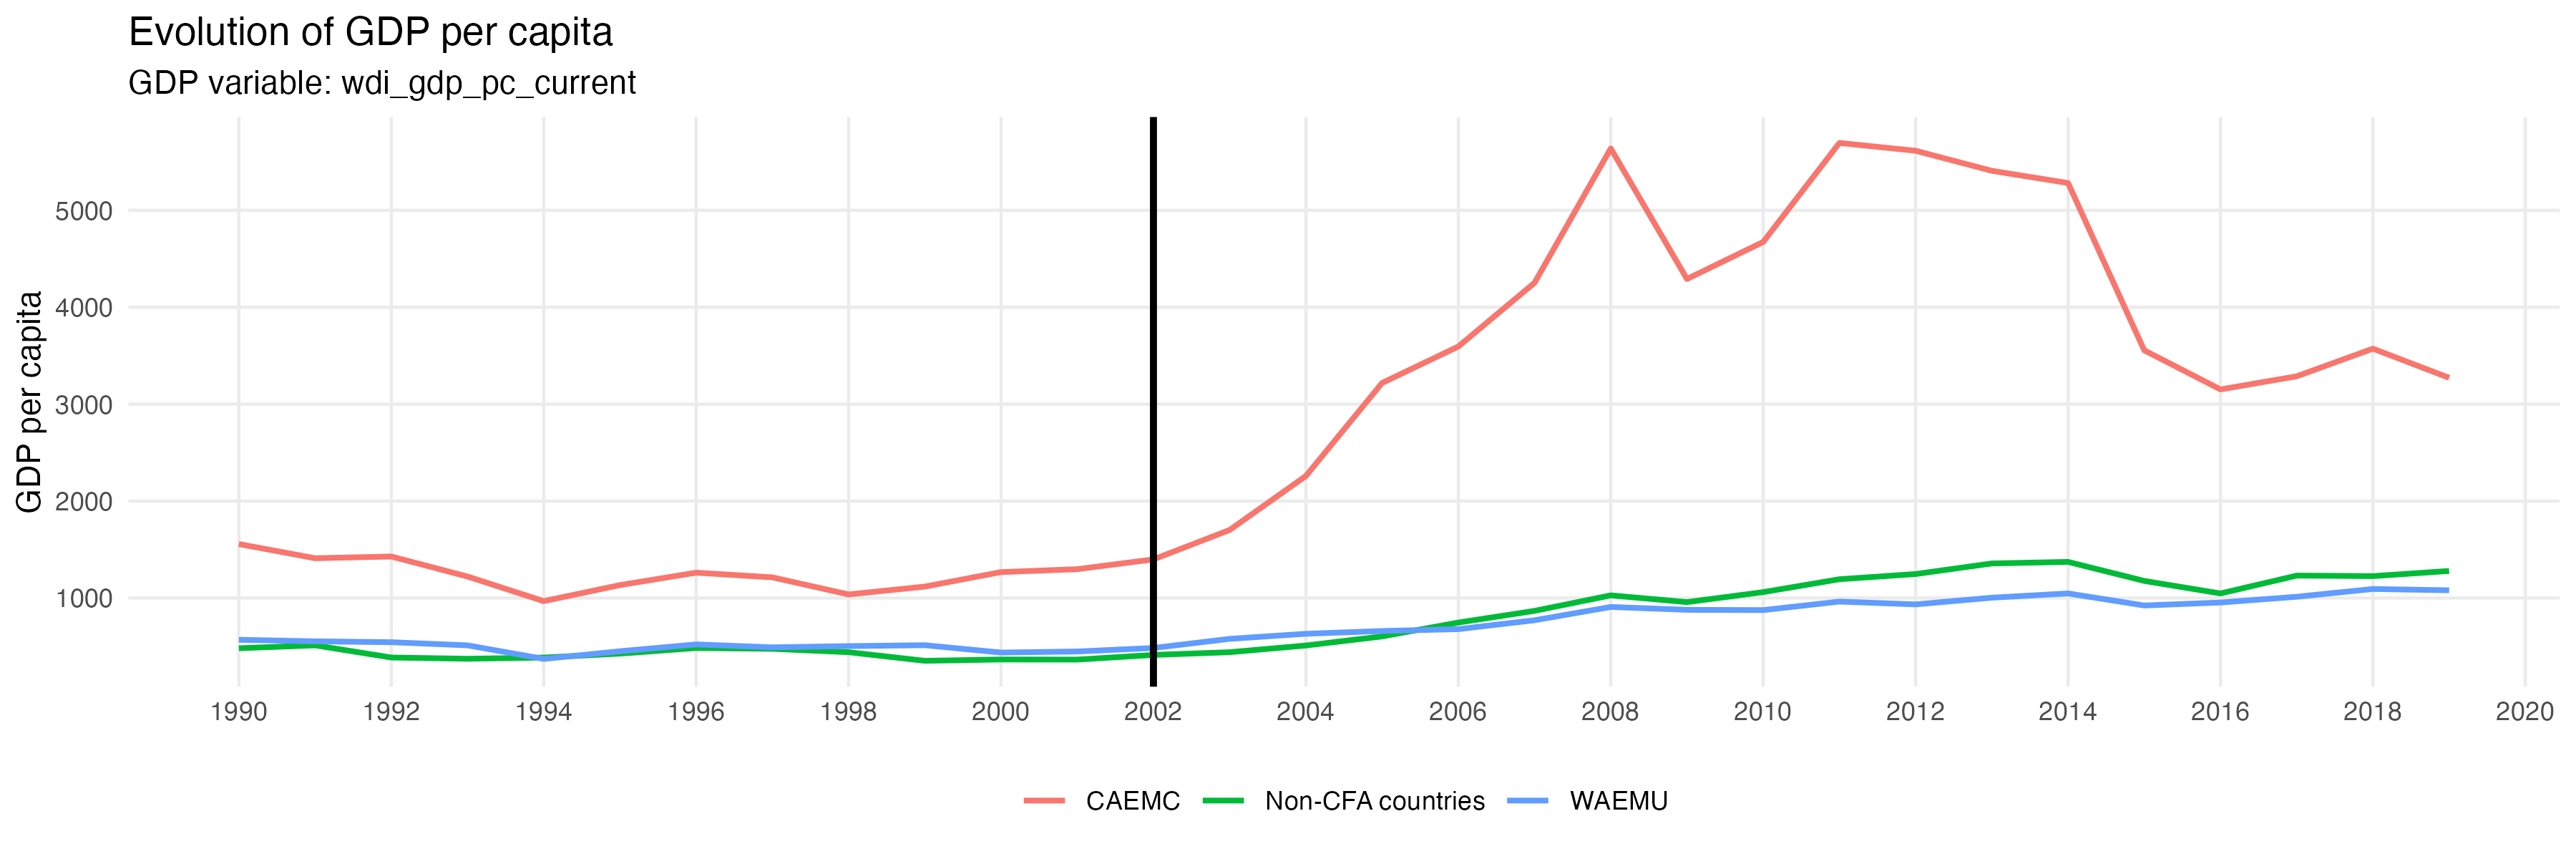
\includegraphics[width=\textwidth]{../output/figures/gdp_pc_used_regions.png}

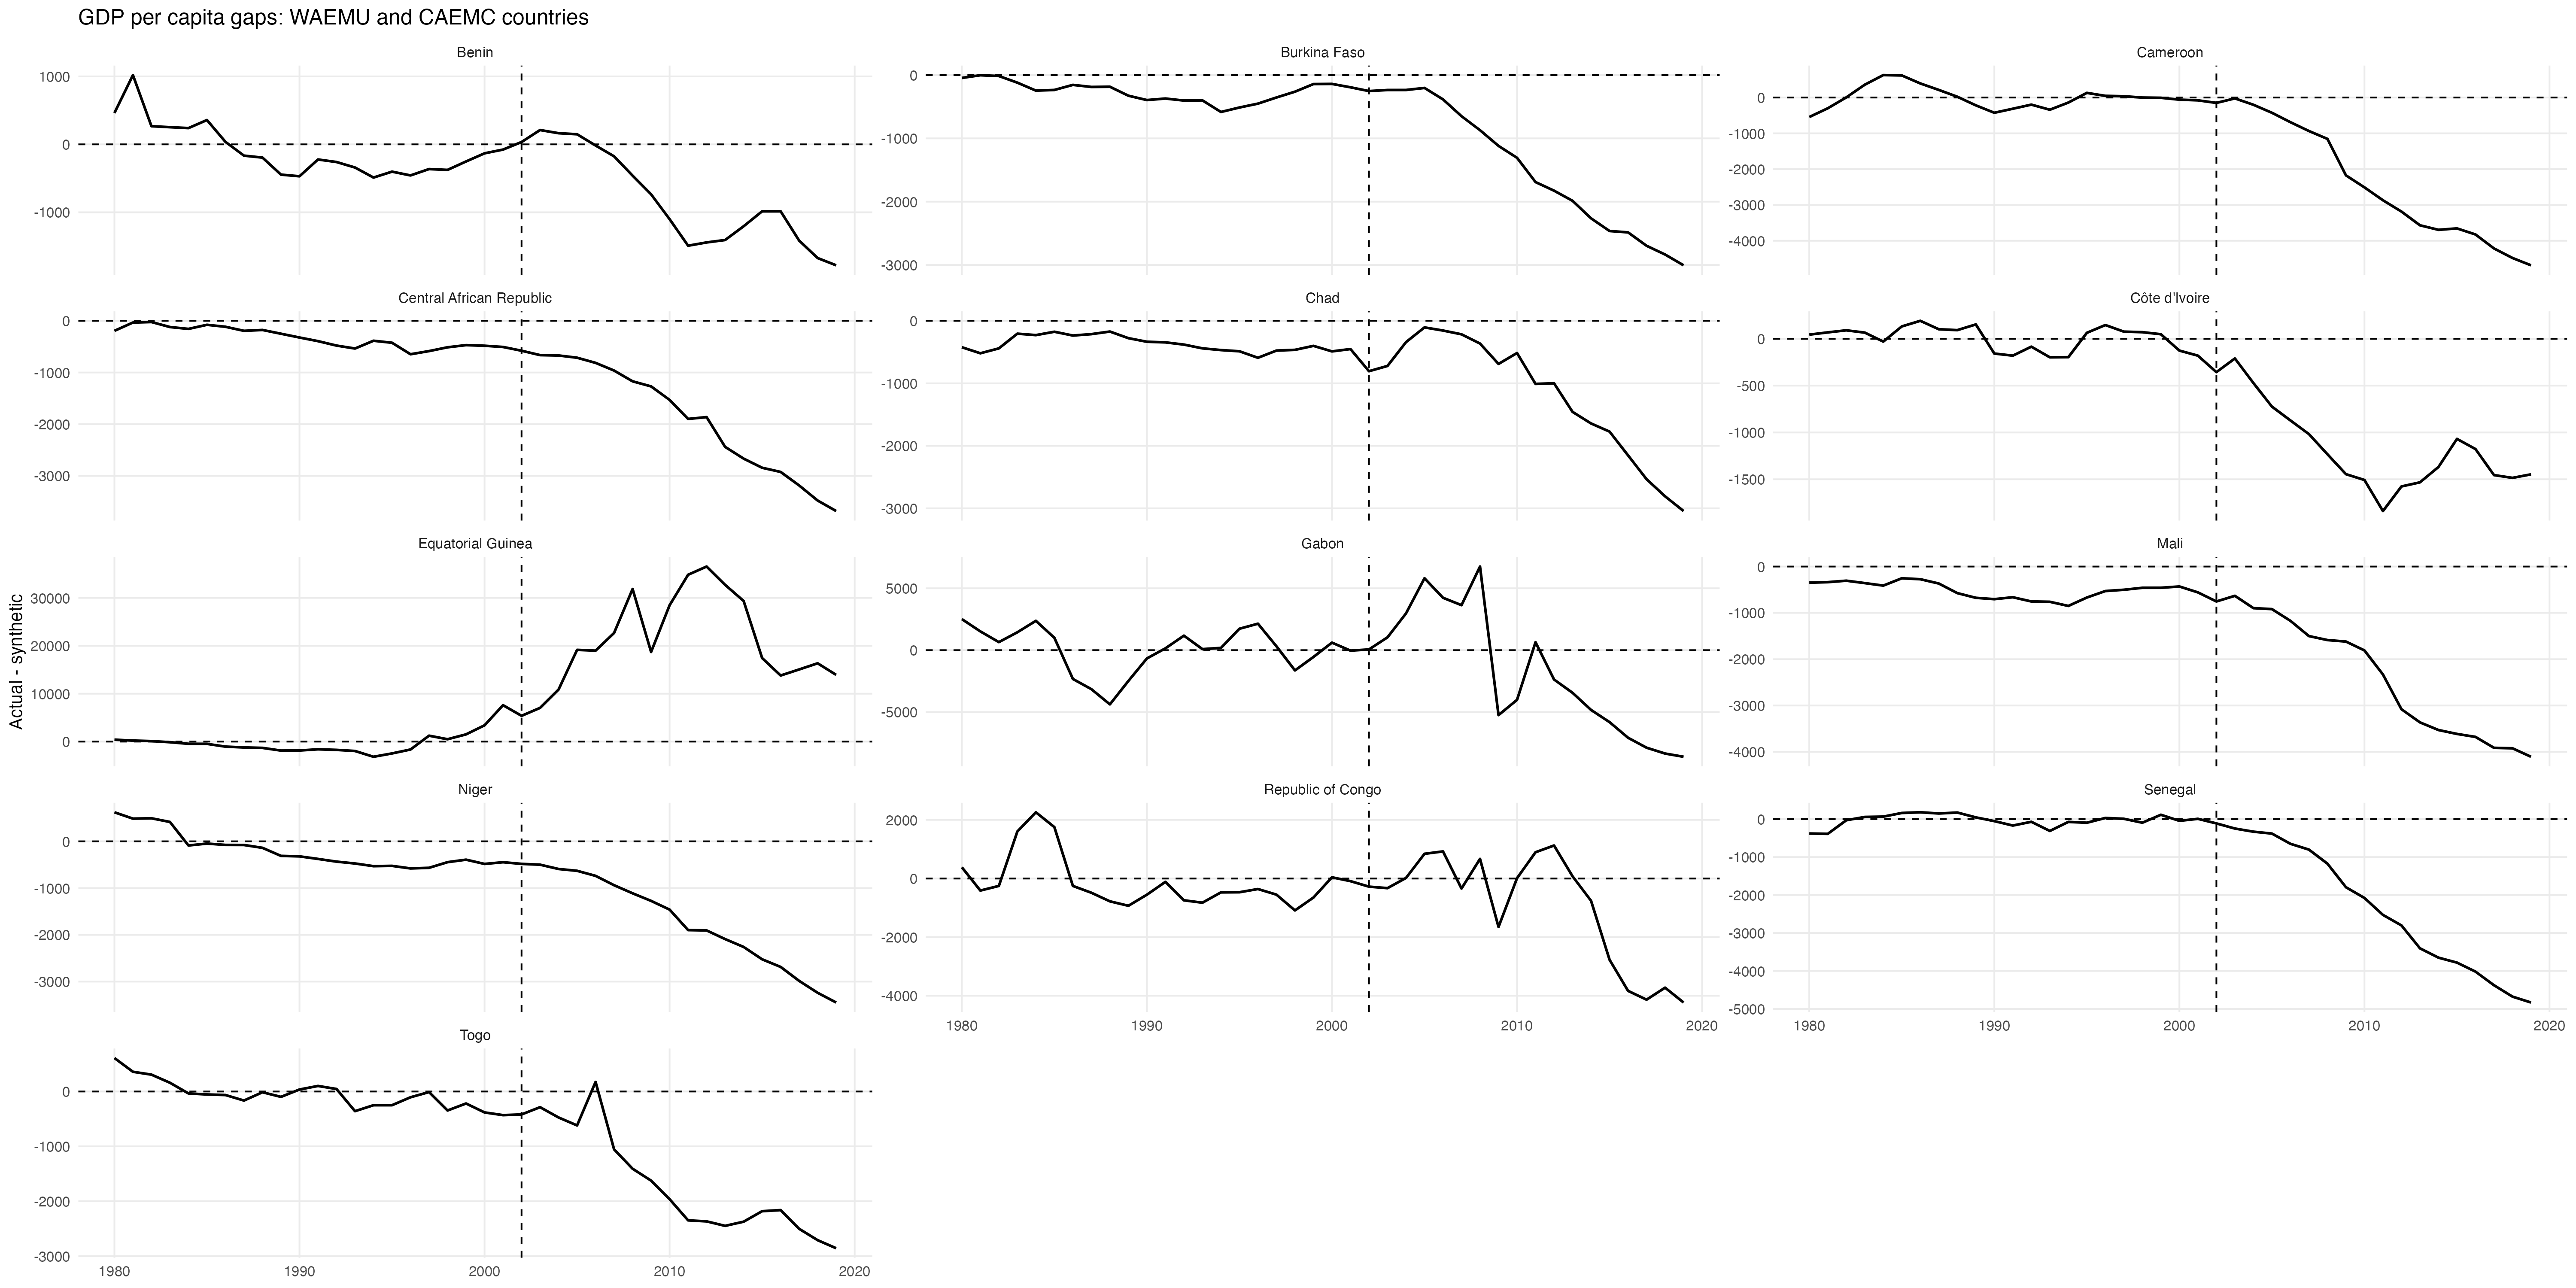
\includegraphics[width=\textwidth]{../output/figures/scm_gaps_all_treated.png}

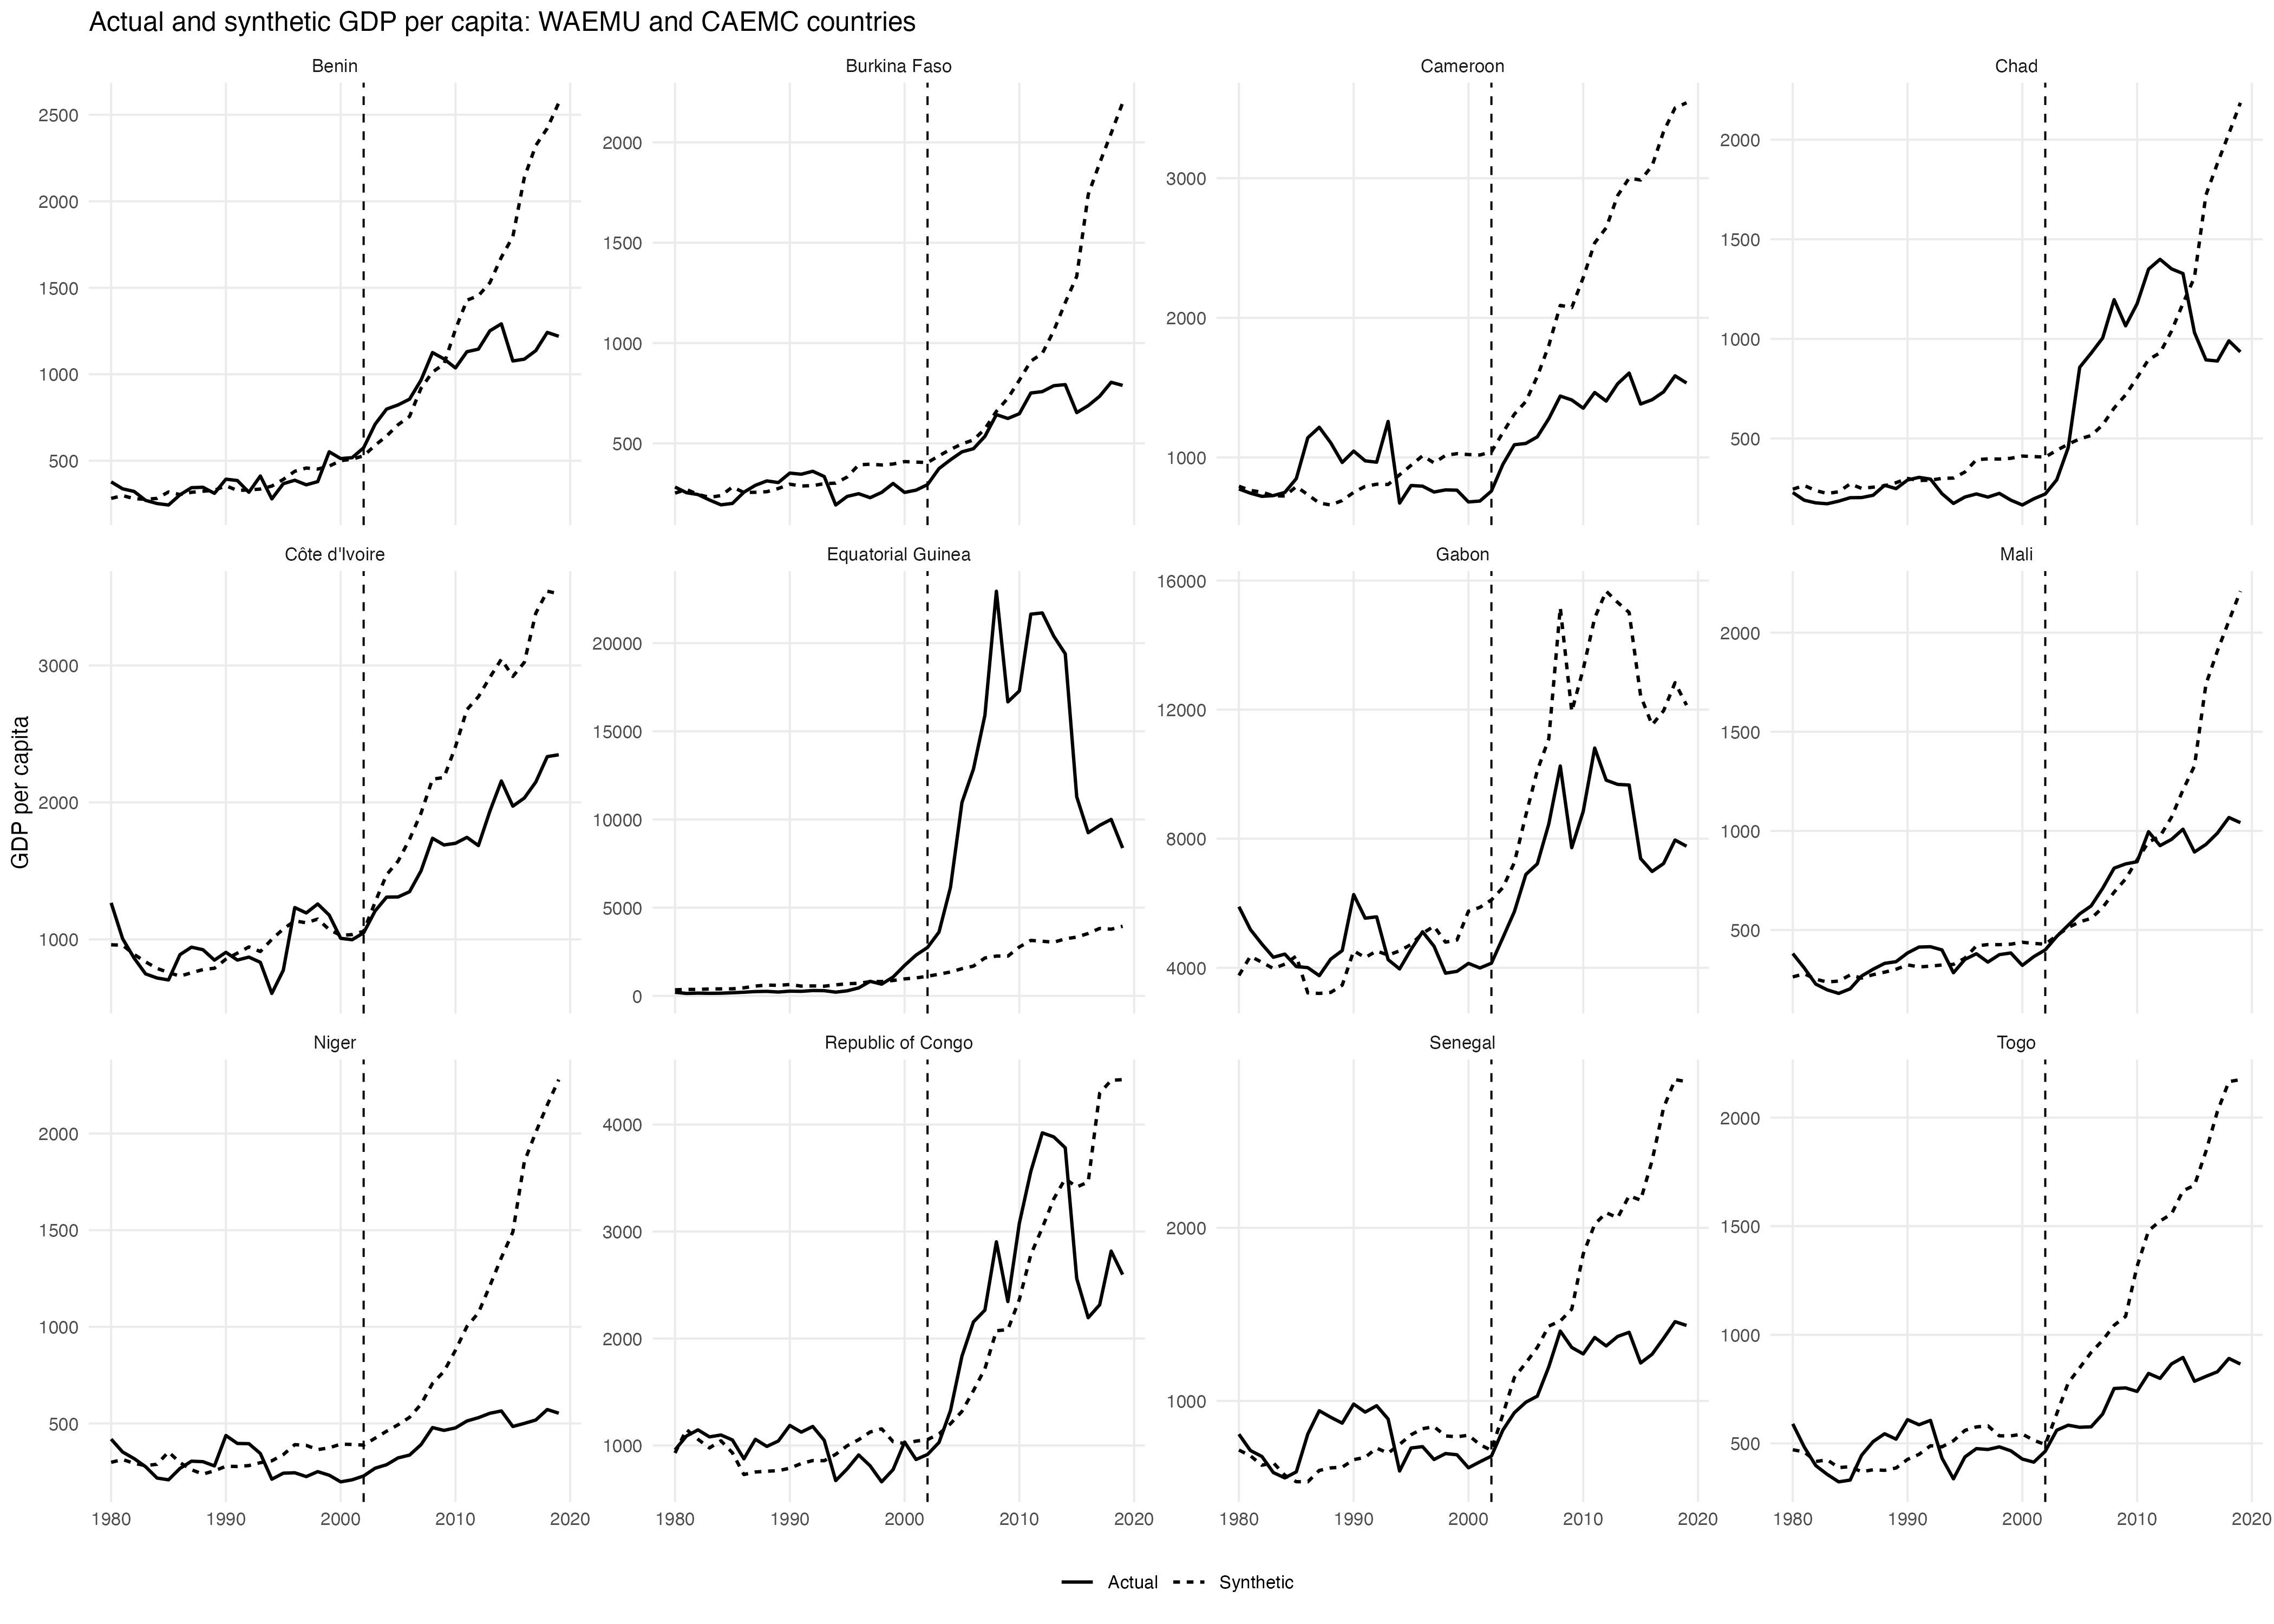
\includegraphics[width=\textwidth]{../output/figures/scm_paths_all_treated.png}

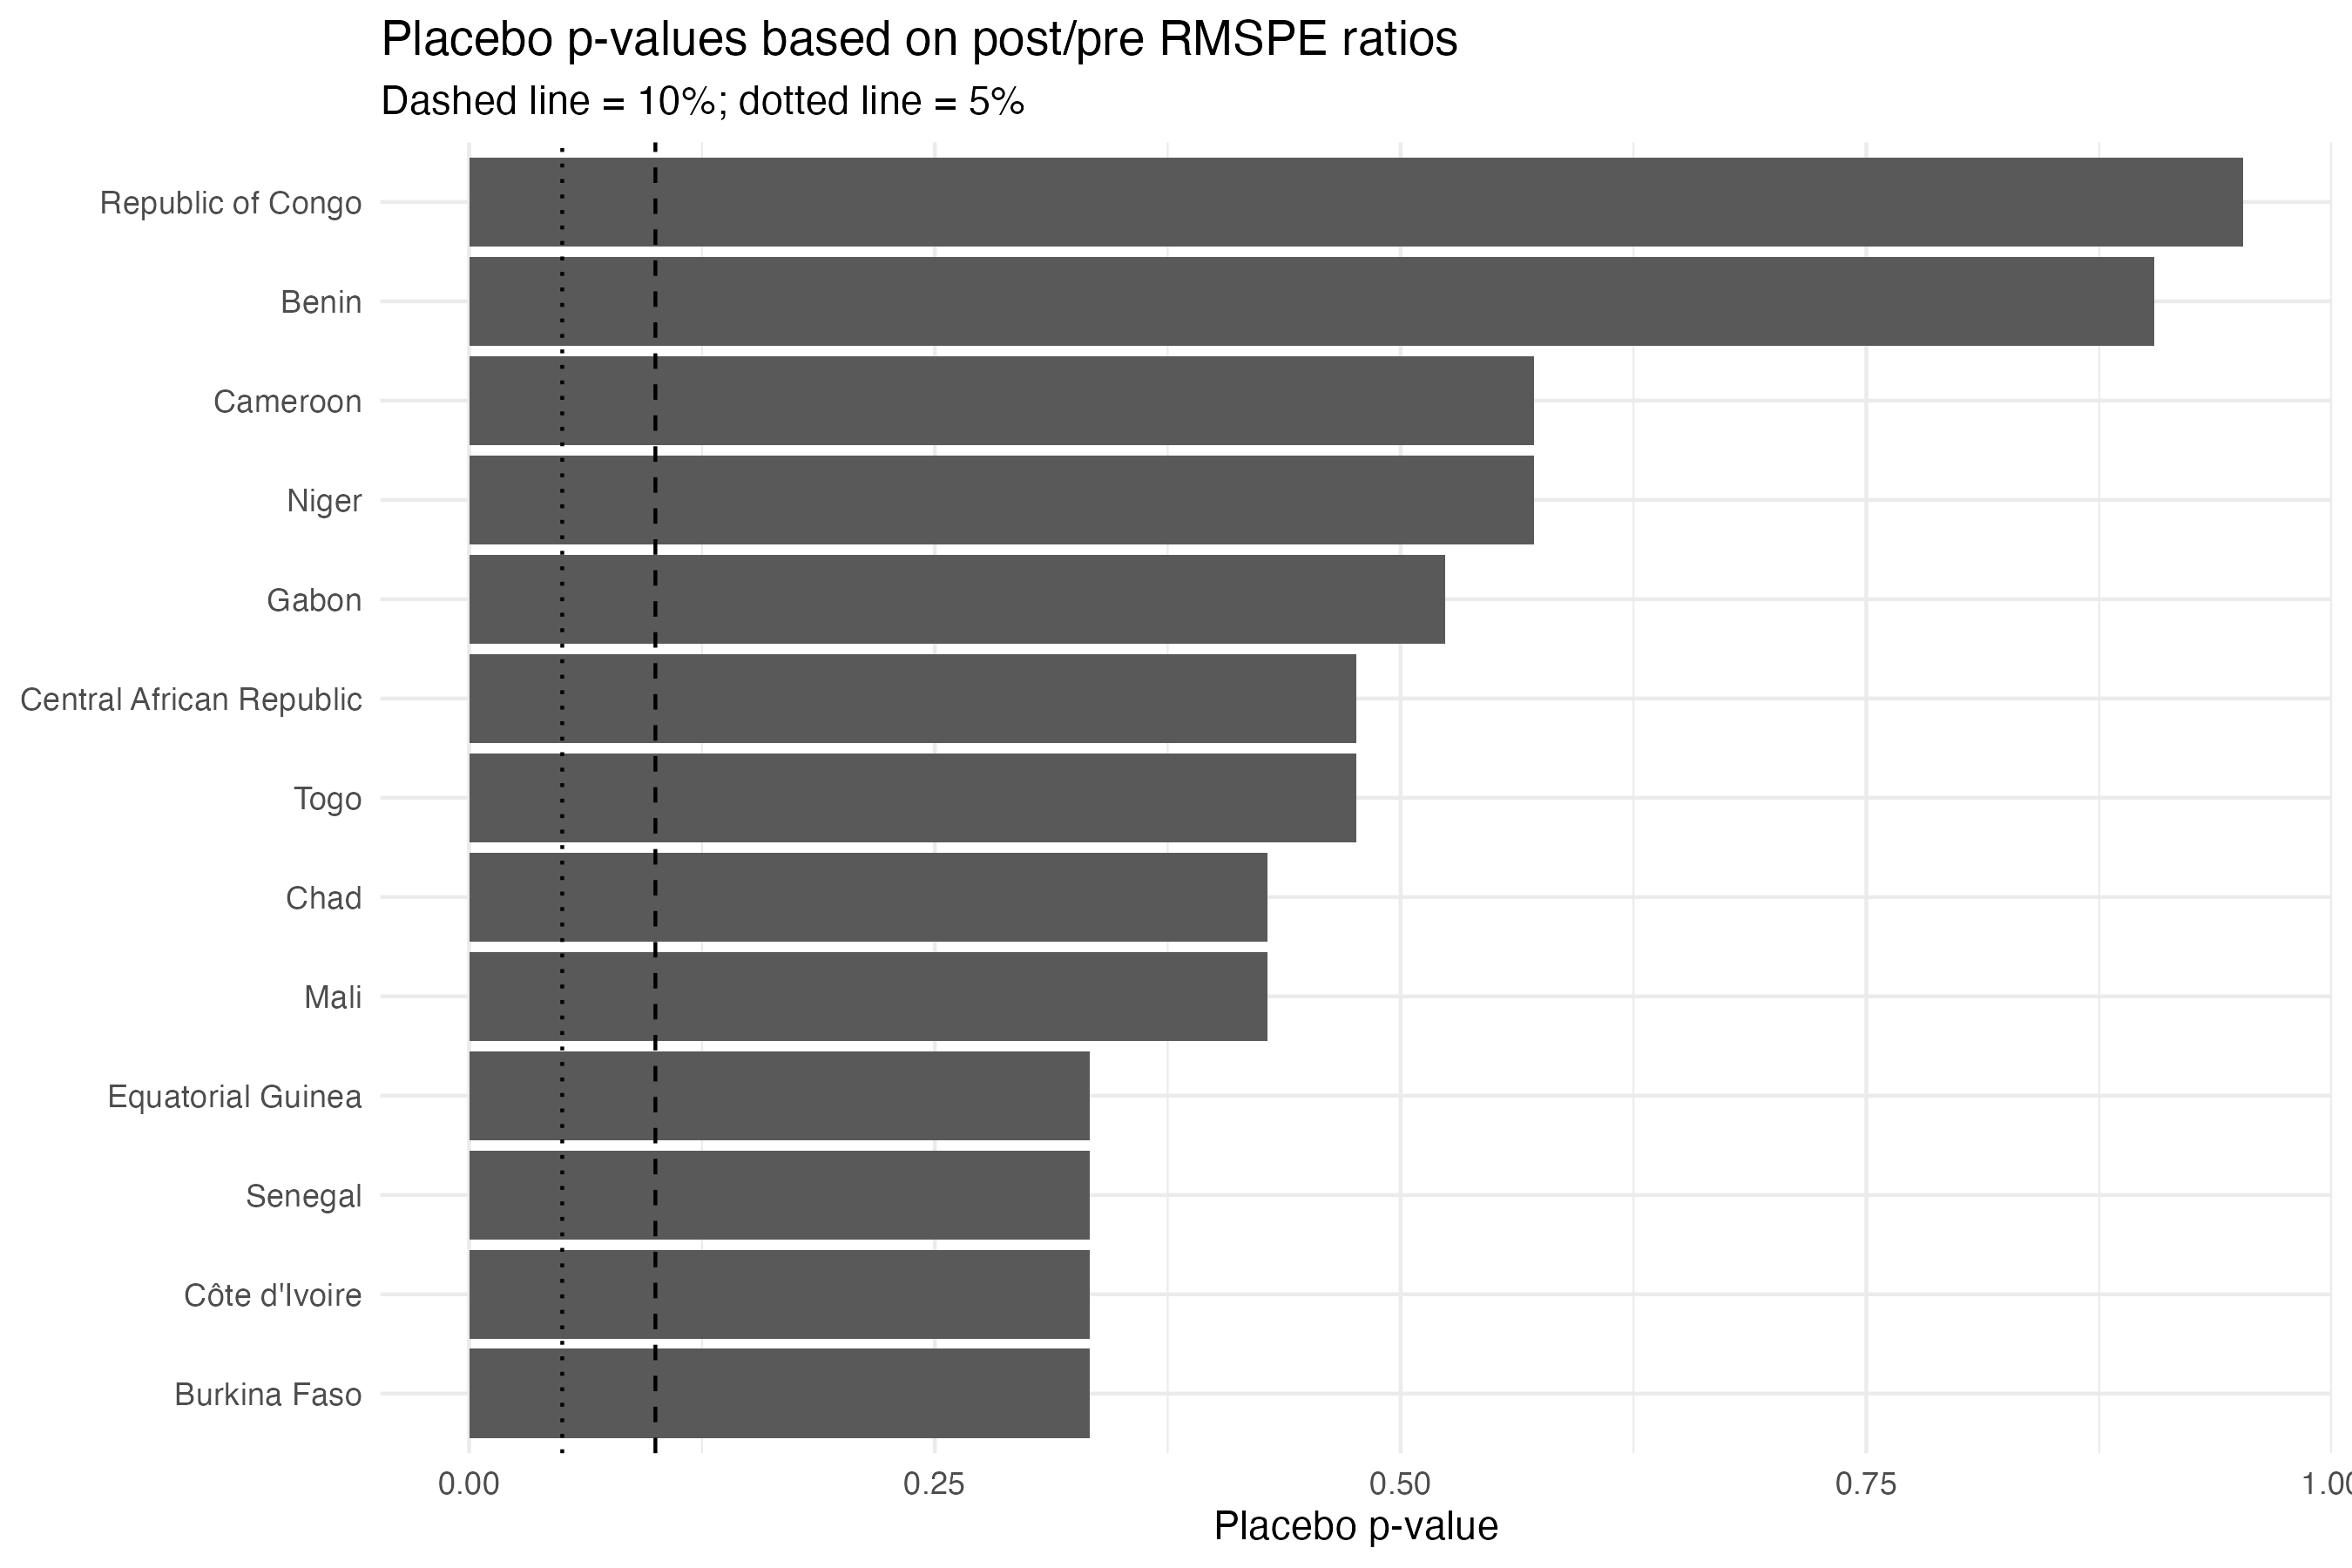
\includegraphics[width=\textwidth]{../output/figures/scm_placebo_pvalues_rmspe_ratio.png}

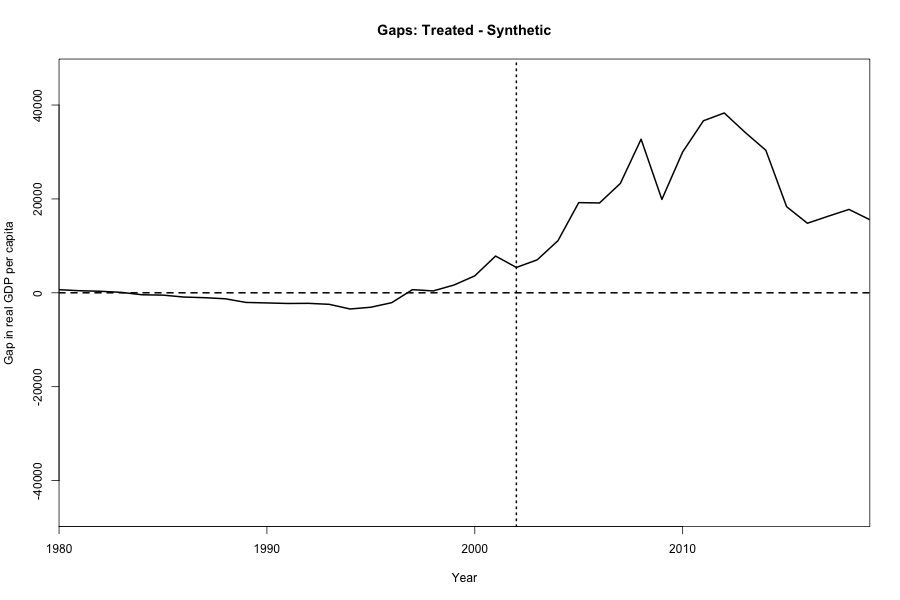
\includegraphics[width=\textwidth]{../output/figures/scm_gap_GNQ.png}

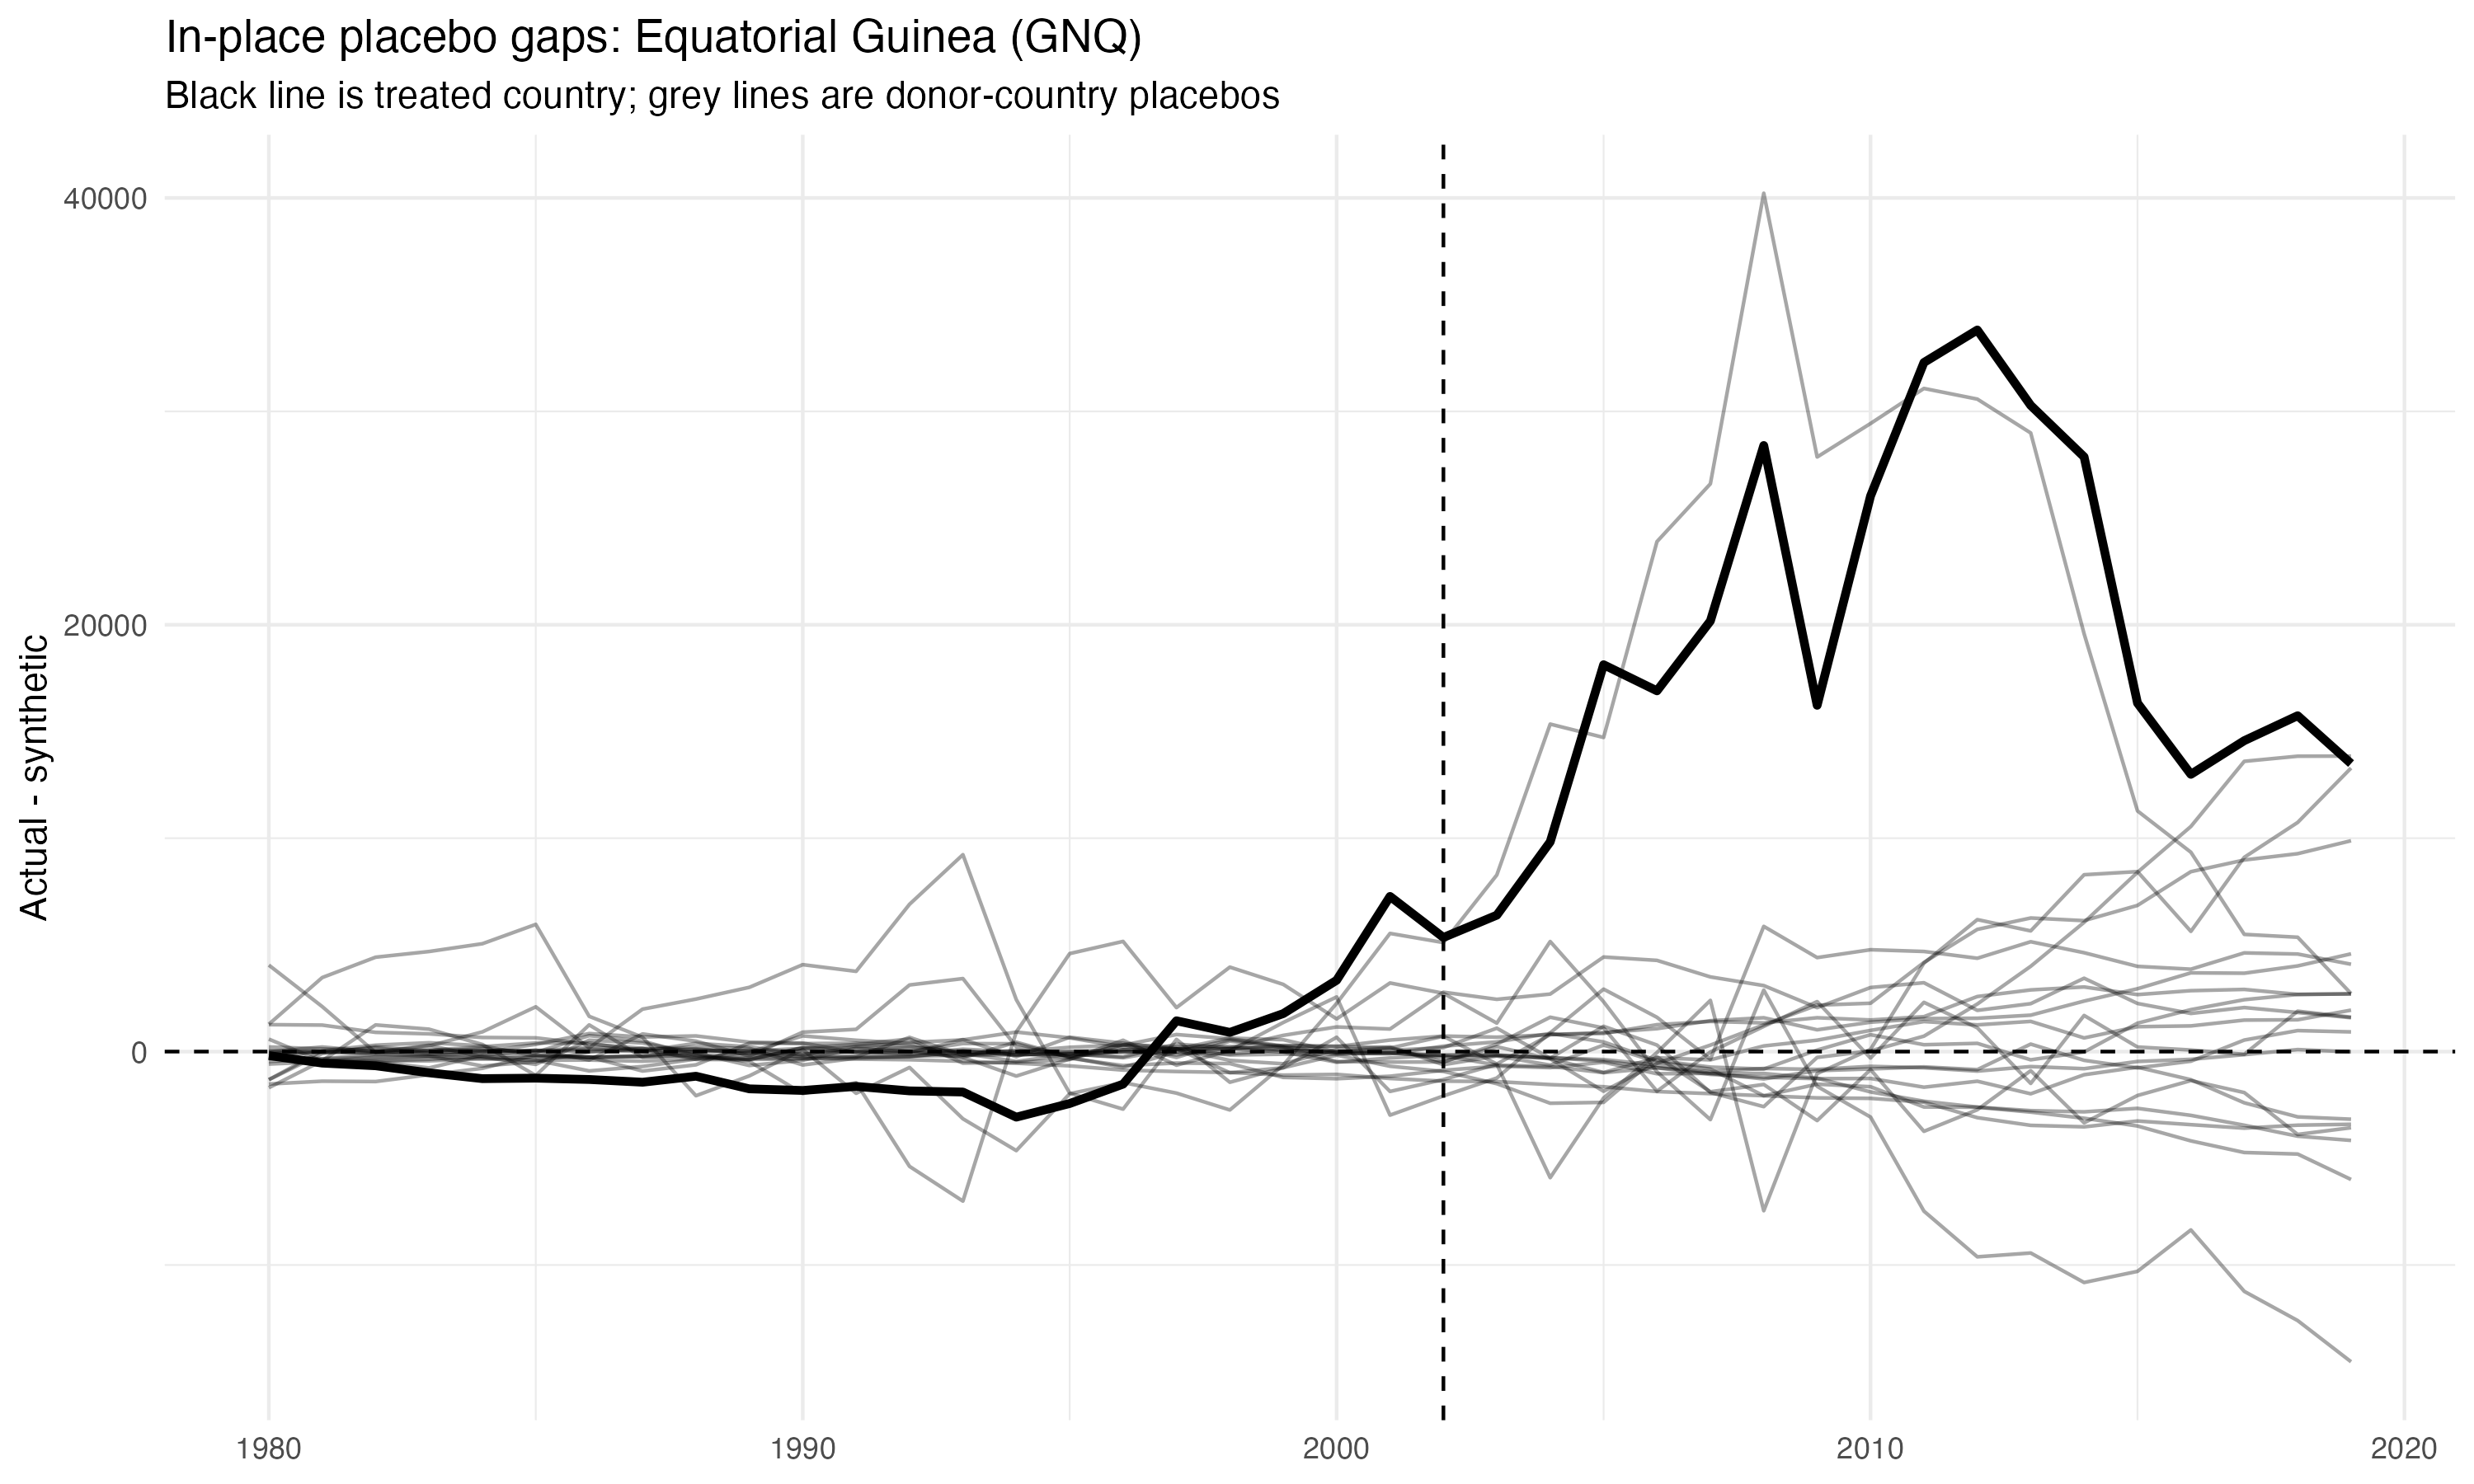
\includegraphics[width=\textwidth]{../output/figures/scm_placebo_gaps_GNQ.png}

\section{Extension Tables}

\begin{landscape}
\begin{table}

\caption{Extension SCM summary for trade outcomes}
\centering
\begin{tabular}[t]{lllrrrrrl}
\toprule
outcome & treated\_iso3c & treated\_country & pre\_rmspe & post\_rmspe & rmspe\_ratio & avg\_post\_gap & avg\_abs\_post\_gap & outcome\_label\\
\midrule
MEU & BEN & Benin & 4.740438 & 15.617041 & 3.2944296 & -13.8408334 & 13.840833 & Imports from EU (\% of total imports)\\
MEU & BFA & Burkina Faso & 5.205163 & 14.847303 & 2.8524186 & -14.3512625 & 14.351263 & Imports from EU (\% of total imports)\\
MEU & CAF & Central African Republic & 12.029886 & 24.439553 & 2.0315698 & -21.1949729 & 21.714439 & Imports from EU (\% of total imports)\\
MEU & CIV & Côte d'Ivoire & 5.132861 & 18.955975 & 3.6930623 & -17.1880613 & 17.188061 & Imports from EU (\% of total imports)\\
MEU & CMR & Cameroon & 9.125855 & 26.179158 & 2.8686799 & -25.0141587 & 25.014159 & Imports from EU (\% of total imports)\\
\addlinespace
MEU & COG & Republic of Congo & 14.375437 & 37.836069 & 2.6319943 & -36.2932688 & 36.293269 & Imports from EU (\% of total imports)\\
MEU & GAB & Gabon & 7.555036 & 30.751044 & 4.0702711 & -21.5499129 & 24.434454 & Imports from EU (\% of total imports)\\
MEU & GNQ & Equatorial Guinea & 17.363994 & 23.870283 & 1.3747001 & -23.0139310 & 23.013931 & Imports from EU (\% of total imports)\\
MEU & MLI & Mali & 10.233356 & 10.643753 & 1.0401039 & -9.6770227 & 9.677023 & Imports from EU (\% of total imports)\\
MEU & NER & Niger & 7.016746 & 9.172159 & 1.3071812 & -8.0933944 & 8.610415 & Imports from EU (\% of total imports)\\
\addlinespace
MEU & SEN & Senegal & 3.668794 & 12.681645 & 3.4566250 & -11.8079709 & 11.807971 & Imports from EU (\% of total imports)\\
MEU & TCD & Chad & 10.329470 & 25.724796 & 2.4904275 & -23.1336859 & 23.262100 & Imports from EU (\% of total imports)\\
MEU & TGO & Togo & 10.970151 & 16.456914 & 1.5001538 & -14.3598300 & 14.359830 & Imports from EU (\% of total imports)\\
XEU & BEN & Benin & 20.203927 & 16.245284 & 0.8040657 & -16.0536464 & 16.053646 & Exports to EU (\% of total exports)\\
XEU & BFA & Burkina Faso & 8.860764 & 24.476528 & 2.7623495 & -21.8872756 & 23.559216 & Exports to EU (\% of total exports)\\
\addlinespace
XEU & CAF & Central African Republic & 22.332967 & 16.361209 & 0.7326035 & -3.7435440 & 13.077108 & Exports to EU (\% of total exports)\\
XEU & CIV & Côte d'Ivoire & 6.277816 & 14.528041 & 2.3141872 & -13.8755376 & 13.875538 & Exports to EU (\% of total exports)\\
XEU & CMR & Cameroon & 14.318287 & 6.591509 & 0.4603560 & -1.0068068 & 5.260558 & Exports to EU (\% of total exports)\\
XEU & COG & Republic of Congo & 13.225655 & 13.642517 & 1.0315191 & -10.4144214 & 12.755337 & Exports to EU (\% of total exports)\\
XEU & GAB & Gabon & 15.327433 & 12.923145 & 0.8431383 & -11.8499627 & 11.849963 & Exports to EU (\% of total exports)\\
\addlinespace
XEU & GNQ & Equatorial Guinea & 29.864246 & 32.023694 & 1.0723088 & -30.8151028 & 30.815103 & Exports to EU (\% of total exports)\\
XEU & MLI & Mali & 14.845509 & 26.343900 & 1.7745367 & -25.8672286 & 25.867229 & Exports to EU (\% of total exports)\\
XEU & NER & Niger & 12.137954 & 20.813455 & 1.7147416 & -18.4445869 & 18.444587 & Exports to EU (\% of total exports)\\
XEU & SEN & Senegal & 5.393509 & 24.955852 & 4.6270159 & -24.2435584 & 24.243558 & Exports to EU (\% of total exports)\\
XEU & TCD & Chad & 16.434477 & 49.902716 & 3.0364652 & -47.2601214 & 47.460121 & Exports to EU (\% of total exports)\\
\addlinespace
XEU & TGO & Togo & 17.258511 & 16.784060 & 0.9725092 & -16.1284693 & 16.128469 & Exports to EU (\% of total exports)\\
exports\_gdp & BEN & Benin & 3.361911 & 6.417701 & 1.9089446 & -6.0602666 & 6.060267 & Exports of goods and services (\% of GDP)\\
exports\_gdp & BFA & Burkina Faso & 2.598701 & 6.207541 & 2.3887094 & -5.9584216 & 5.958422 & Exports of goods and services (\% of GDP)\\
exports\_gdp & CAF & Central African Republic & 2.358274 & 13.509221 & 5.7284368 & -12.4497160 & 12.449716 & Exports of goods and services (\% of GDP)\\
exports\_gdp & CIV & Côte d'Ivoire & 5.079209 & 4.147575 & 0.8165790 & -4.0559981 & 4.055998 & Exports of goods and services (\% of GDP)\\
\addlinespace
exports\_gdp & CMR & Cameroon & 4.228425 & 9.232743 & 2.1834943 & -8.4956705 & 8.495670 & Exports of goods and services (\% of GDP)\\
exports\_gdp & COG & Republic of Congo & 10.891082 & 12.119244 & 1.1127677 & 12.0211839 & 12.021184 & Exports of goods and services (\% of GDP)\\
exports\_gdp & GAB & Gabon & 9.949549 & 5.526300 & 0.5554322 & -0.1738516 & 4.987402 & Exports of goods and services (\% of GDP)\\
exports\_gdp & MLI & Mali & 1.644789 & 2.337057 & 1.4208854 & 0.5028868 & 1.973068 & Exports of goods and services (\% of GDP)\\
exports\_gdp & NER & Niger & 4.106919 & 10.403599 & 2.5331885 & -9.9852965 & 9.985297 & Exports of goods and services (\% of GDP)\\
\addlinespace
exports\_gdp & SEN & Senegal & 2.031861 & 6.559557 & 3.2283497 & -5.6486291 & 5.648629 & Exports of goods and services (\% of GDP)\\
exports\_gdp & TCD & Chad & 2.778024 & 20.301452 & 7.3078740 & 14.0960344 & 16.925594 & Exports of goods and services (\% of GDP)\\
exports\_gdp & TGO & Togo & 9.188466 & 12.383933 & 1.3477693 & -12.3162065 & 12.316206 & Exports of goods and services (\% of GDP)\\
imports\_gdp & BEN & Benin & 3.237705 & 12.189825 & 3.7649590 & -11.8696181 & 11.869618 & Imports of goods and services (\% of GDP)\\
imports\_gdp & BFA & Burkina Faso & 2.789236 & 5.928738 & 2.1255779 & -5.7271288 & 5.727129 & Imports of goods and services (\% of GDP)\\
\addlinespace
imports\_gdp & CAF & Central African Republic & 2.093336 & 7.181752 & 3.4307684 & -7.1558313 & 7.155831 & Imports of goods and services (\% of GDP)\\
imports\_gdp & CIV & Côte d'Ivoire & 2.664478 & 3.360270 & 1.2611366 & -2.9158345 & 2.915834 & Imports of goods and services (\% of GDP)\\
imports\_gdp & CMR & Cameroon & 4.239115 & 5.740685 & 1.3542177 & -4.8180605 & 5.061897 & Imports of goods and services (\% of GDP)\\
imports\_gdp & COG & Republic of Congo & 14.629023 & 12.141741 & 0.8299762 & -0.8212777 & 10.073267 & Imports of goods and services (\% of GDP)\\
imports\_gdp & GAB & Gabon & 6.504453 & 15.281396 & 2.3493743 & -13.8042022 & 13.804202 & Imports of goods and services (\% of GDP)\\
\addlinespace
imports\_gdp & MLI & Mali & 4.218661 & 6.111241 & 1.4486211 & -5.5183312 & 5.518331 & Imports of goods and services (\% of GDP)\\
imports\_gdp & NER & Niger & 4.257775 & 2.201008 & 0.5169385 & -1.5541337 & 1.554134 & Imports of goods and services (\% of GDP)\\
imports\_gdp & SEN & Senegal & 3.701995 & 4.113182 & 1.1110717 & 4.1069223 & 4.106922 & Imports of goods and services (\% of GDP)\\
imports\_gdp & TCD & Chad & 5.682360 & 43.505743 & 7.6562802 & 31.1153966 & 32.568526 & Imports of goods and services (\% of GDP)\\
imports\_gdp & TGO & Togo & 8.467835 & 3.004984 & 0.3548705 & -1.7871499 & 2.603954 & Imports of goods and services (\% of GDP)\\
\addlinespace
trade\_openness & BEN & Benin & 5.648168 & 19.699045 & 3.4876876 & -18.8839147 & 18.883915 & Trade openness (\% of GDP)\\
trade\_openness & BFA & Burkina Faso & 4.301250 & 11.058926 & 2.5710960 & -10.6249525 & 10.624952 & Trade openness (\% of GDP)\\
trade\_openness & CAF & Central African Republic & 4.843208 & 21.335653 & 4.4052728 & -20.5333222 & 20.533322 & Trade openness (\% of GDP)\\
trade\_openness & CIV & Côte d'Ivoire & 6.974370 & 7.702623 & 1.1044185 & -7.1014379 & 7.101438 & Trade openness (\% of GDP)\\
trade\_openness & CMR & Cameroon & 8.472586 & 11.241547 & 1.3268142 & -10.5937178 & 10.593718 & Trade openness (\% of GDP)\\
\addlinespace
trade\_openness & COG & Republic of Congo & 22.320958 & 14.290754 & 0.6402393 & 9.3890419 & 11.411153 & Trade openness (\% of GDP)\\
trade\_openness & GAB & Gabon & 9.588430 & 11.899685 & 1.2410463 & -11.8039598 & 11.803960 & Trade openness (\% of GDP)\\
trade\_openness & MLI & Mali & 4.777973 & 4.220420 & 0.8833075 & -1.6417605 & 3.244533 & Trade openness (\% of GDP)\\
trade\_openness & NER & Niger & 9.196864 & 13.061180 & 1.4201776 & -12.8551125 & 12.855113 & Trade openness (\% of GDP)\\
trade\_openness & SEN & Senegal & 6.689059 & 5.642009 & 0.8434683 & -4.7272333 & 4.727233 & Trade openness (\% of GDP)\\
\addlinespace
trade\_openness & TCD & Chad & 6.621517 & 52.408849 & 7.9149307 & 48.3301444 & 48.330144 & Trade openness (\% of GDP)\\
trade\_openness & TGO & Togo & 19.015139 & 30.177289 & 1.5870138 & -30.0756582 & 30.075658 & Trade openness (\% of GDP)\\
\bottomrule
\end{tabular}
\end{table}
    
\end{landscape}

\section{Extension Figures}

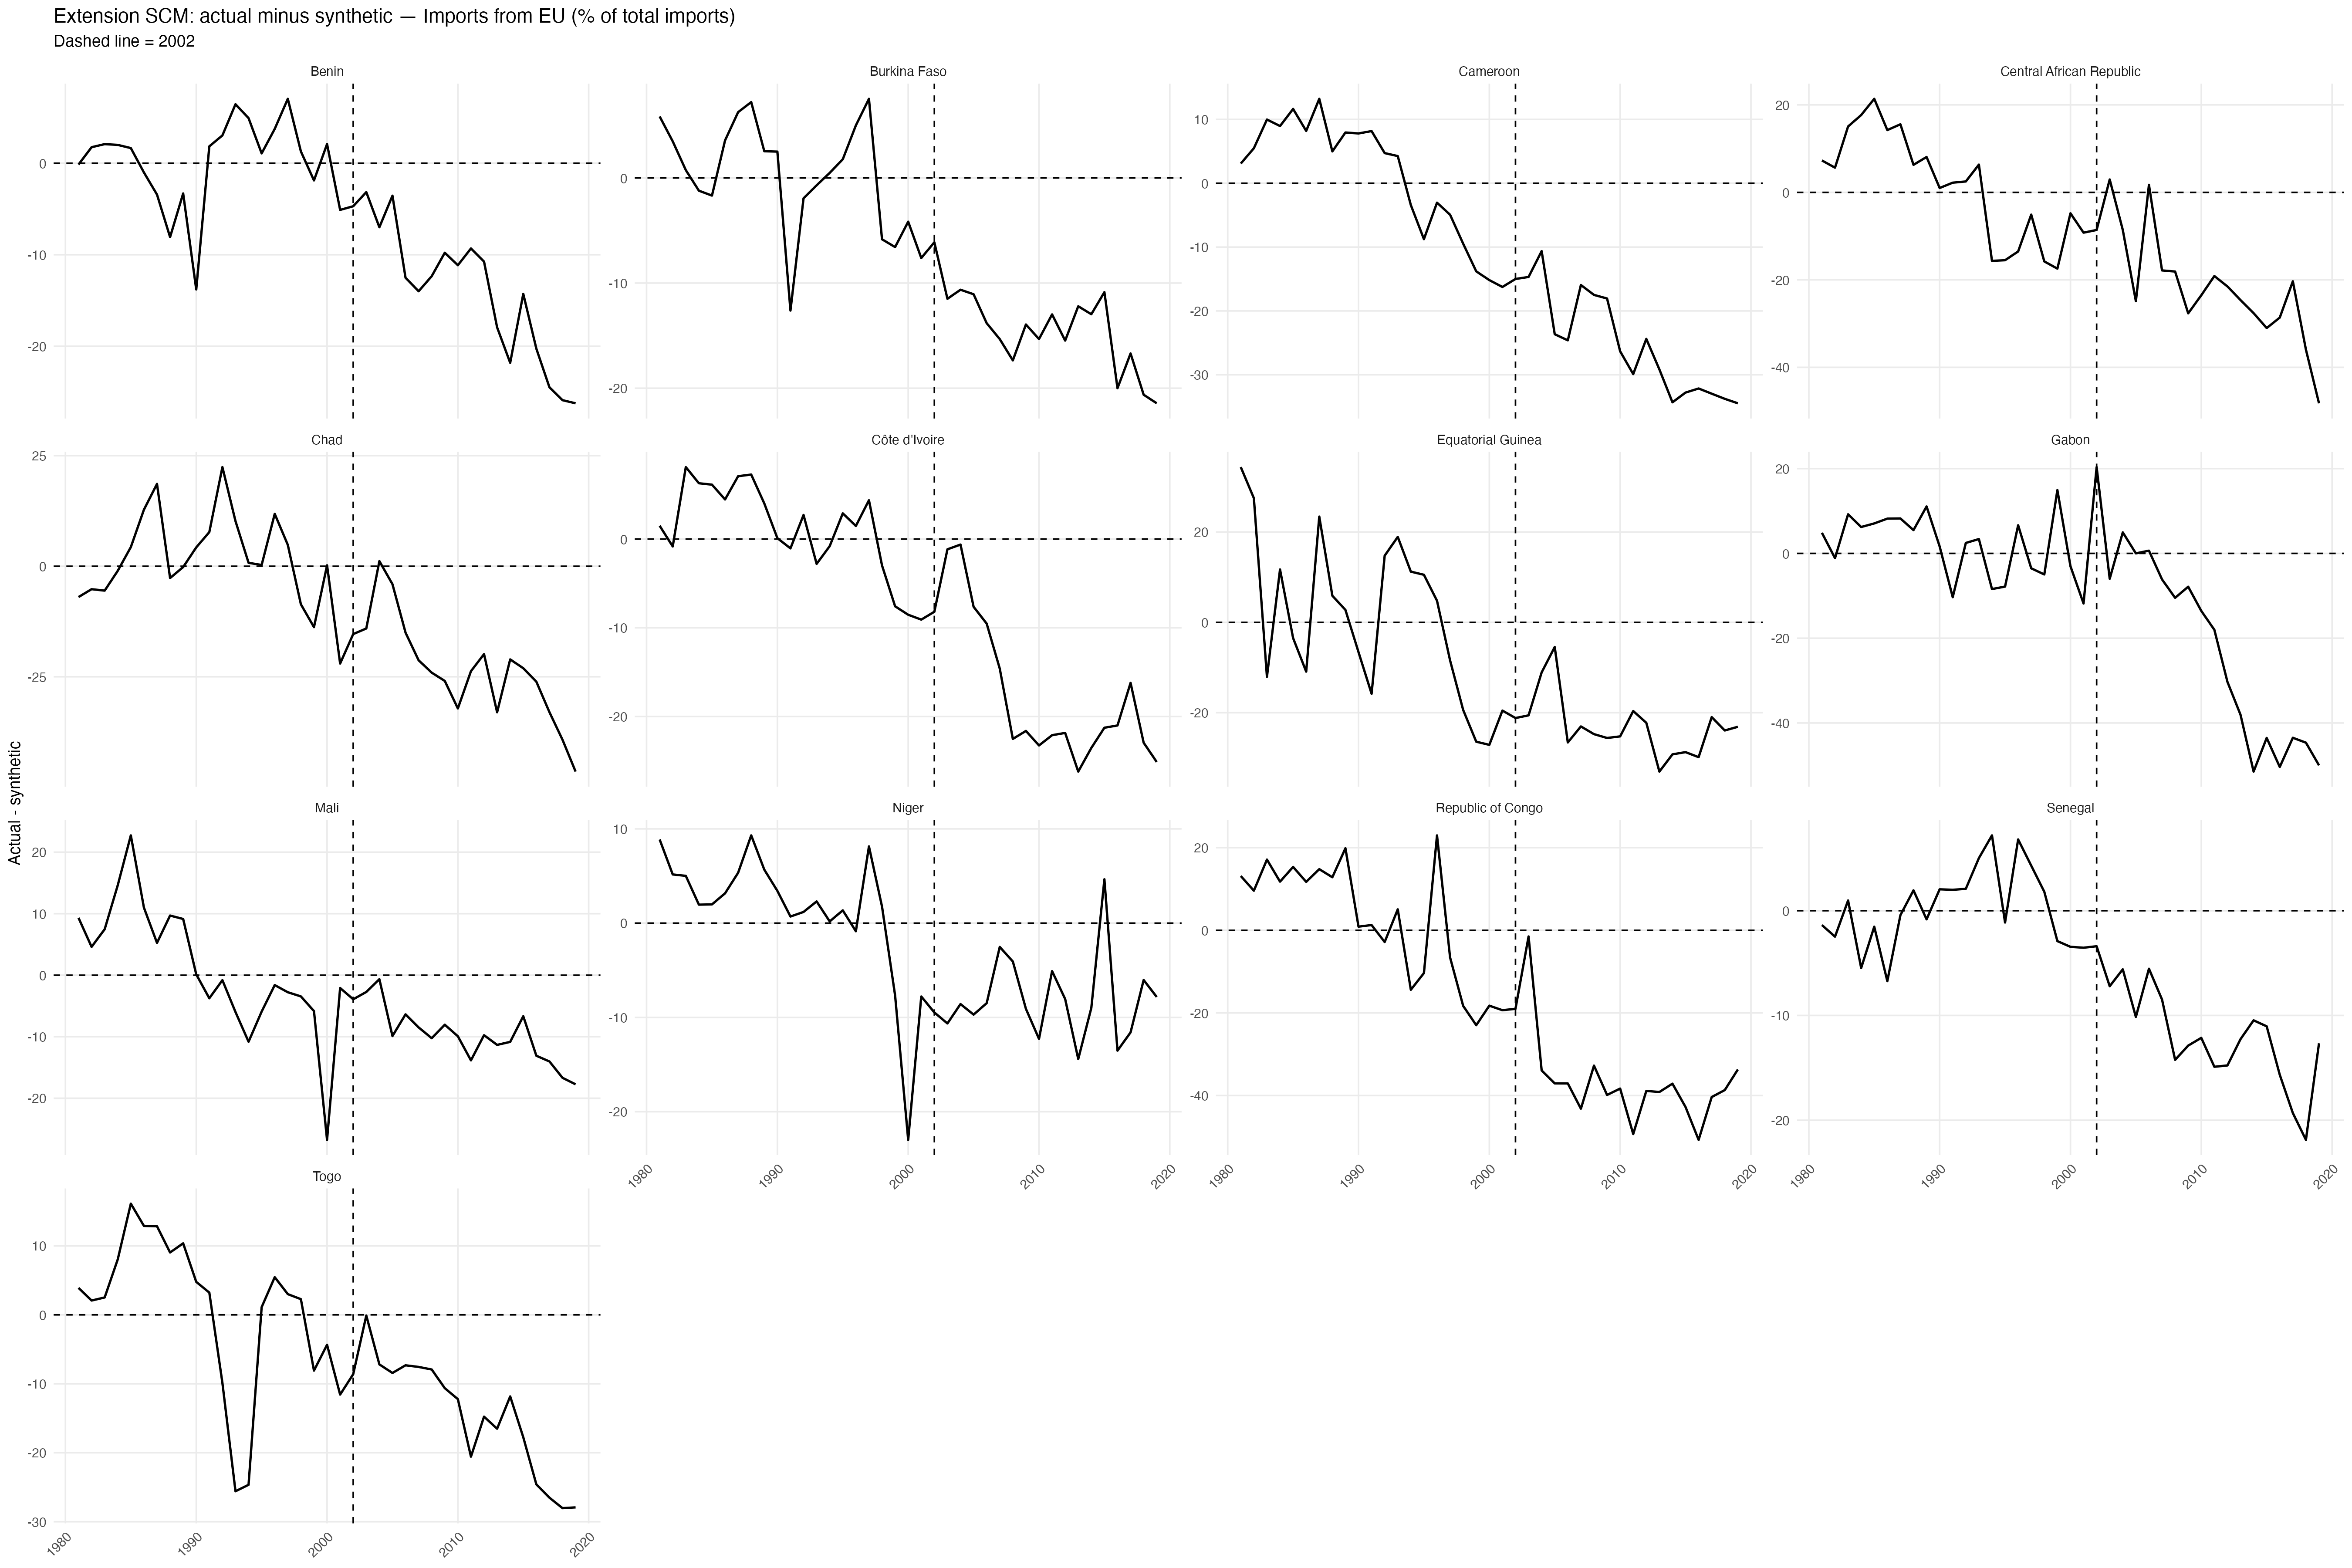
\includegraphics[width=\textwidth]{../output/extension_trade/figures/extension_trade_scm_gaps_MEU.png}

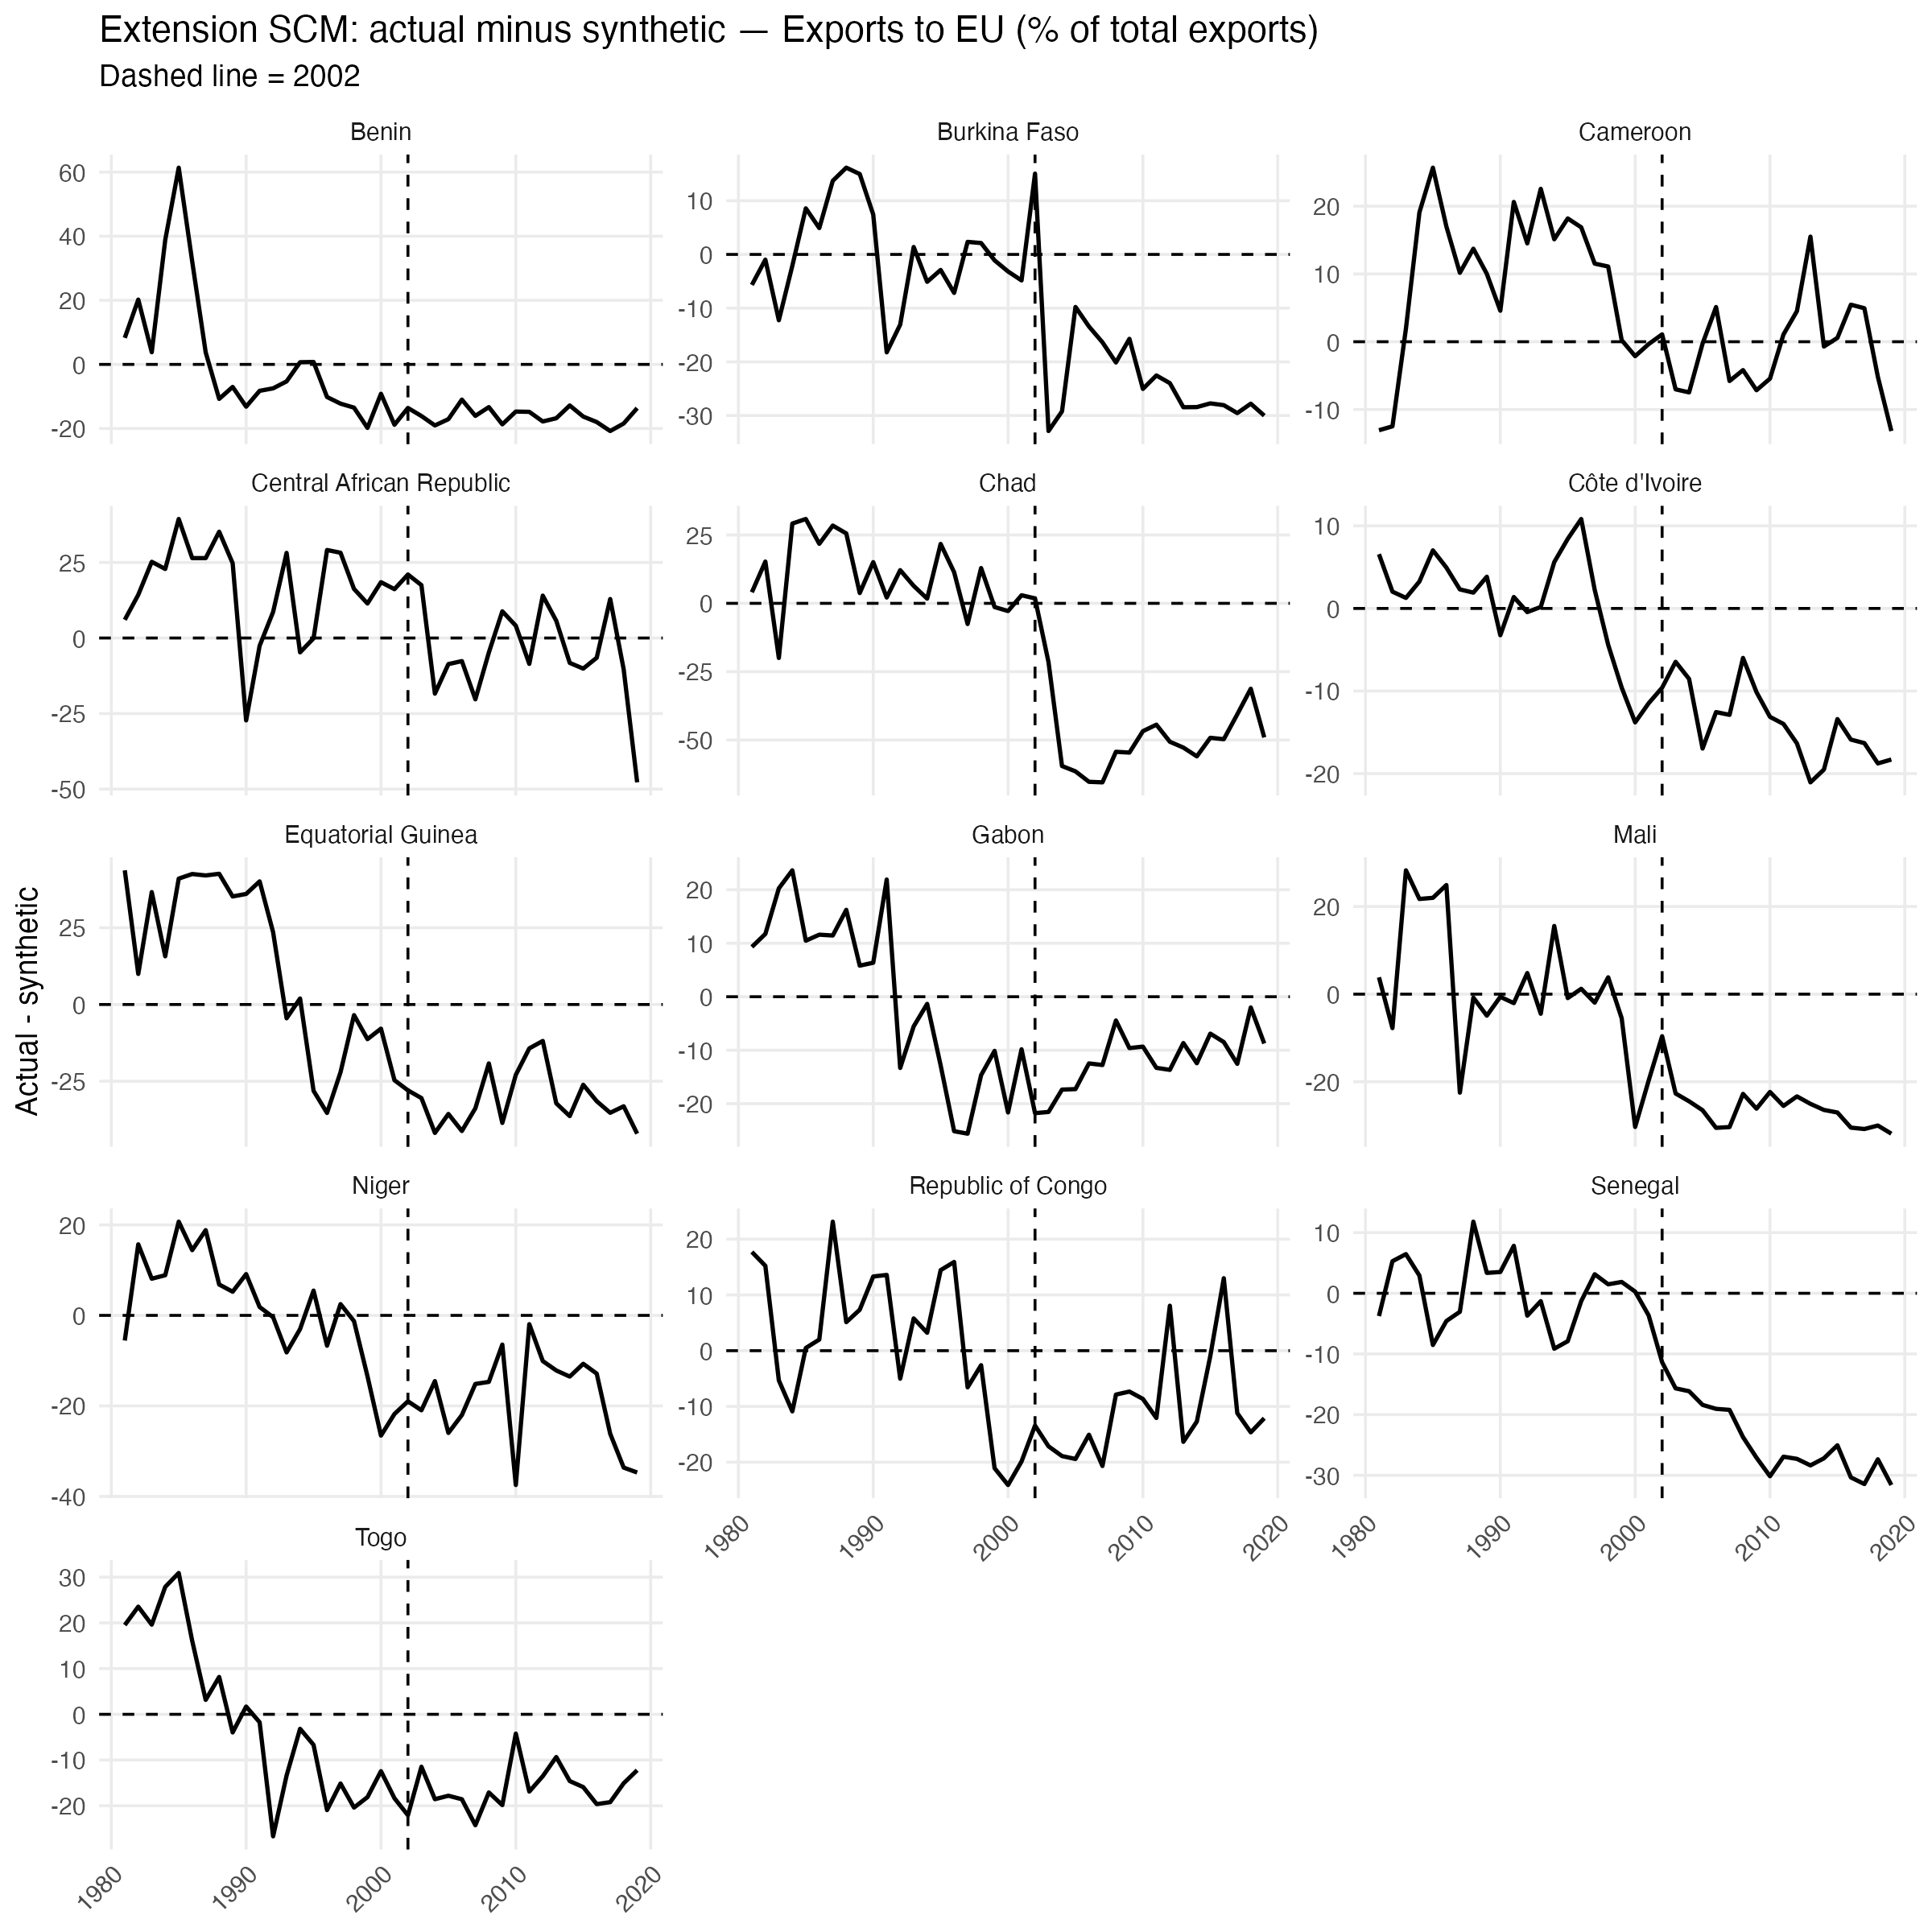
\includegraphics[width=\textwidth]{../output/extension_trade/figures/extension_trade_scm_gaps_XEU.png}

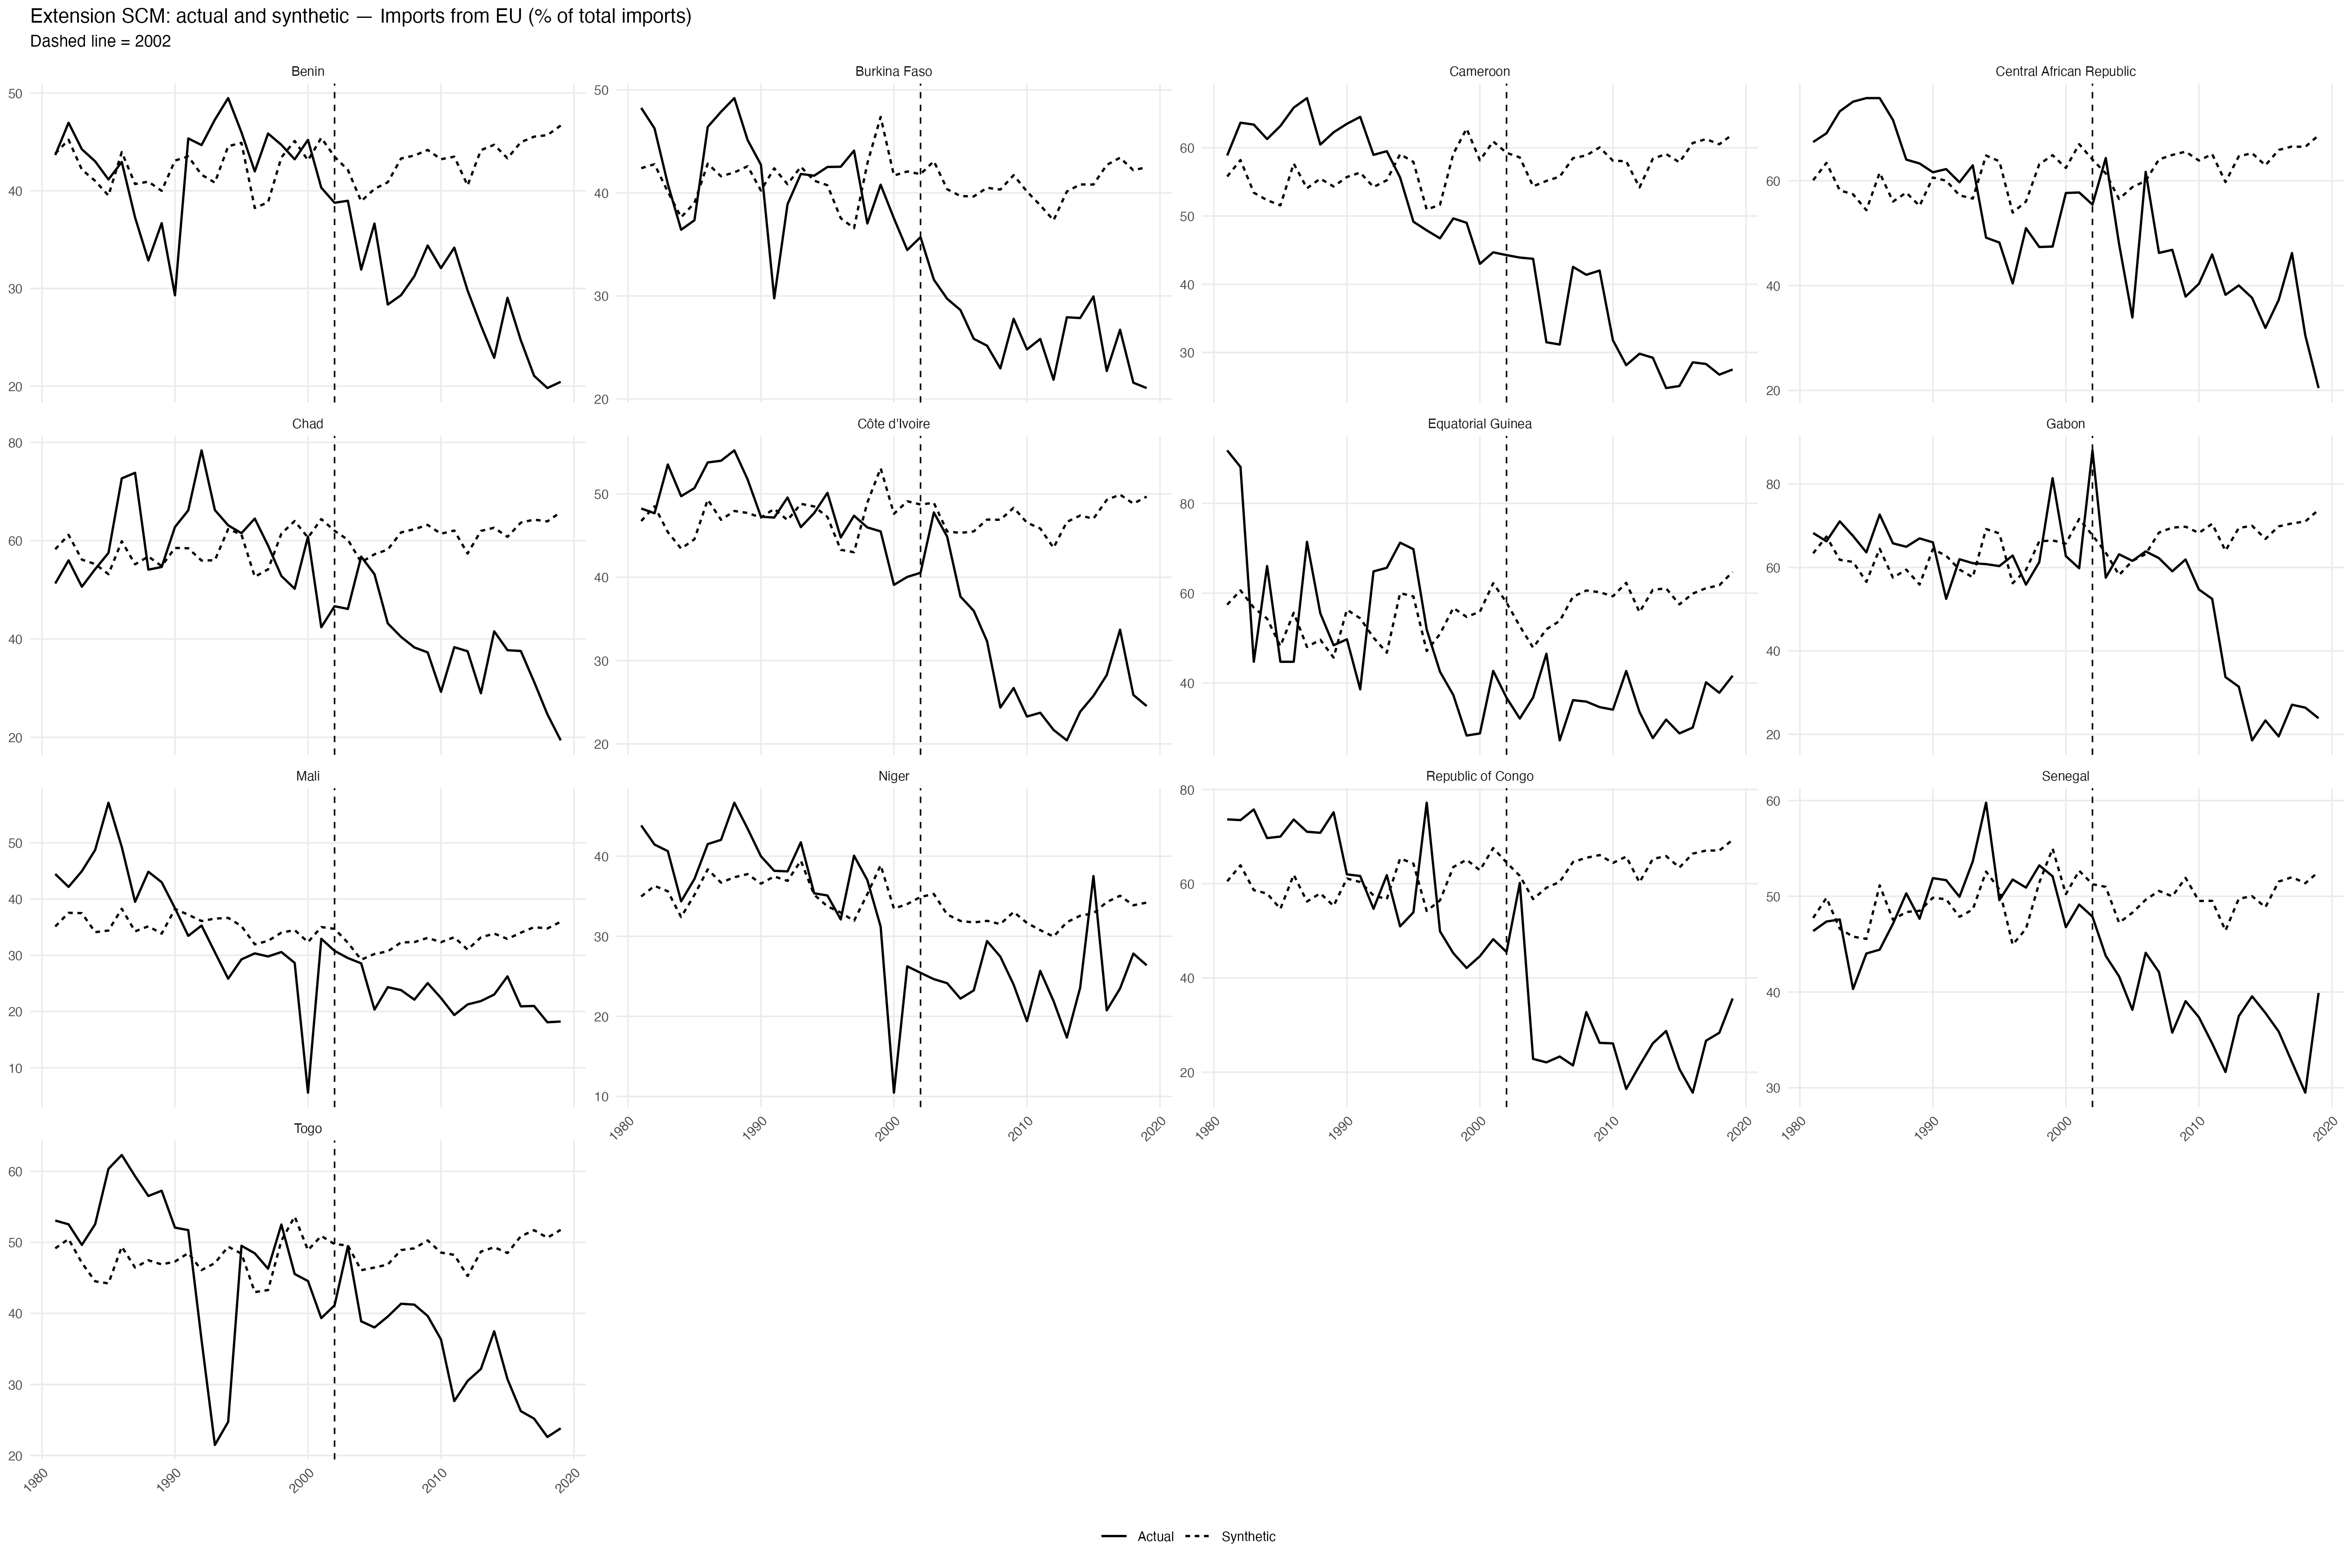
\includegraphics[width=\textwidth]{../output/extension_trade/figures/extension_trade_scm_paths_MEU.png}

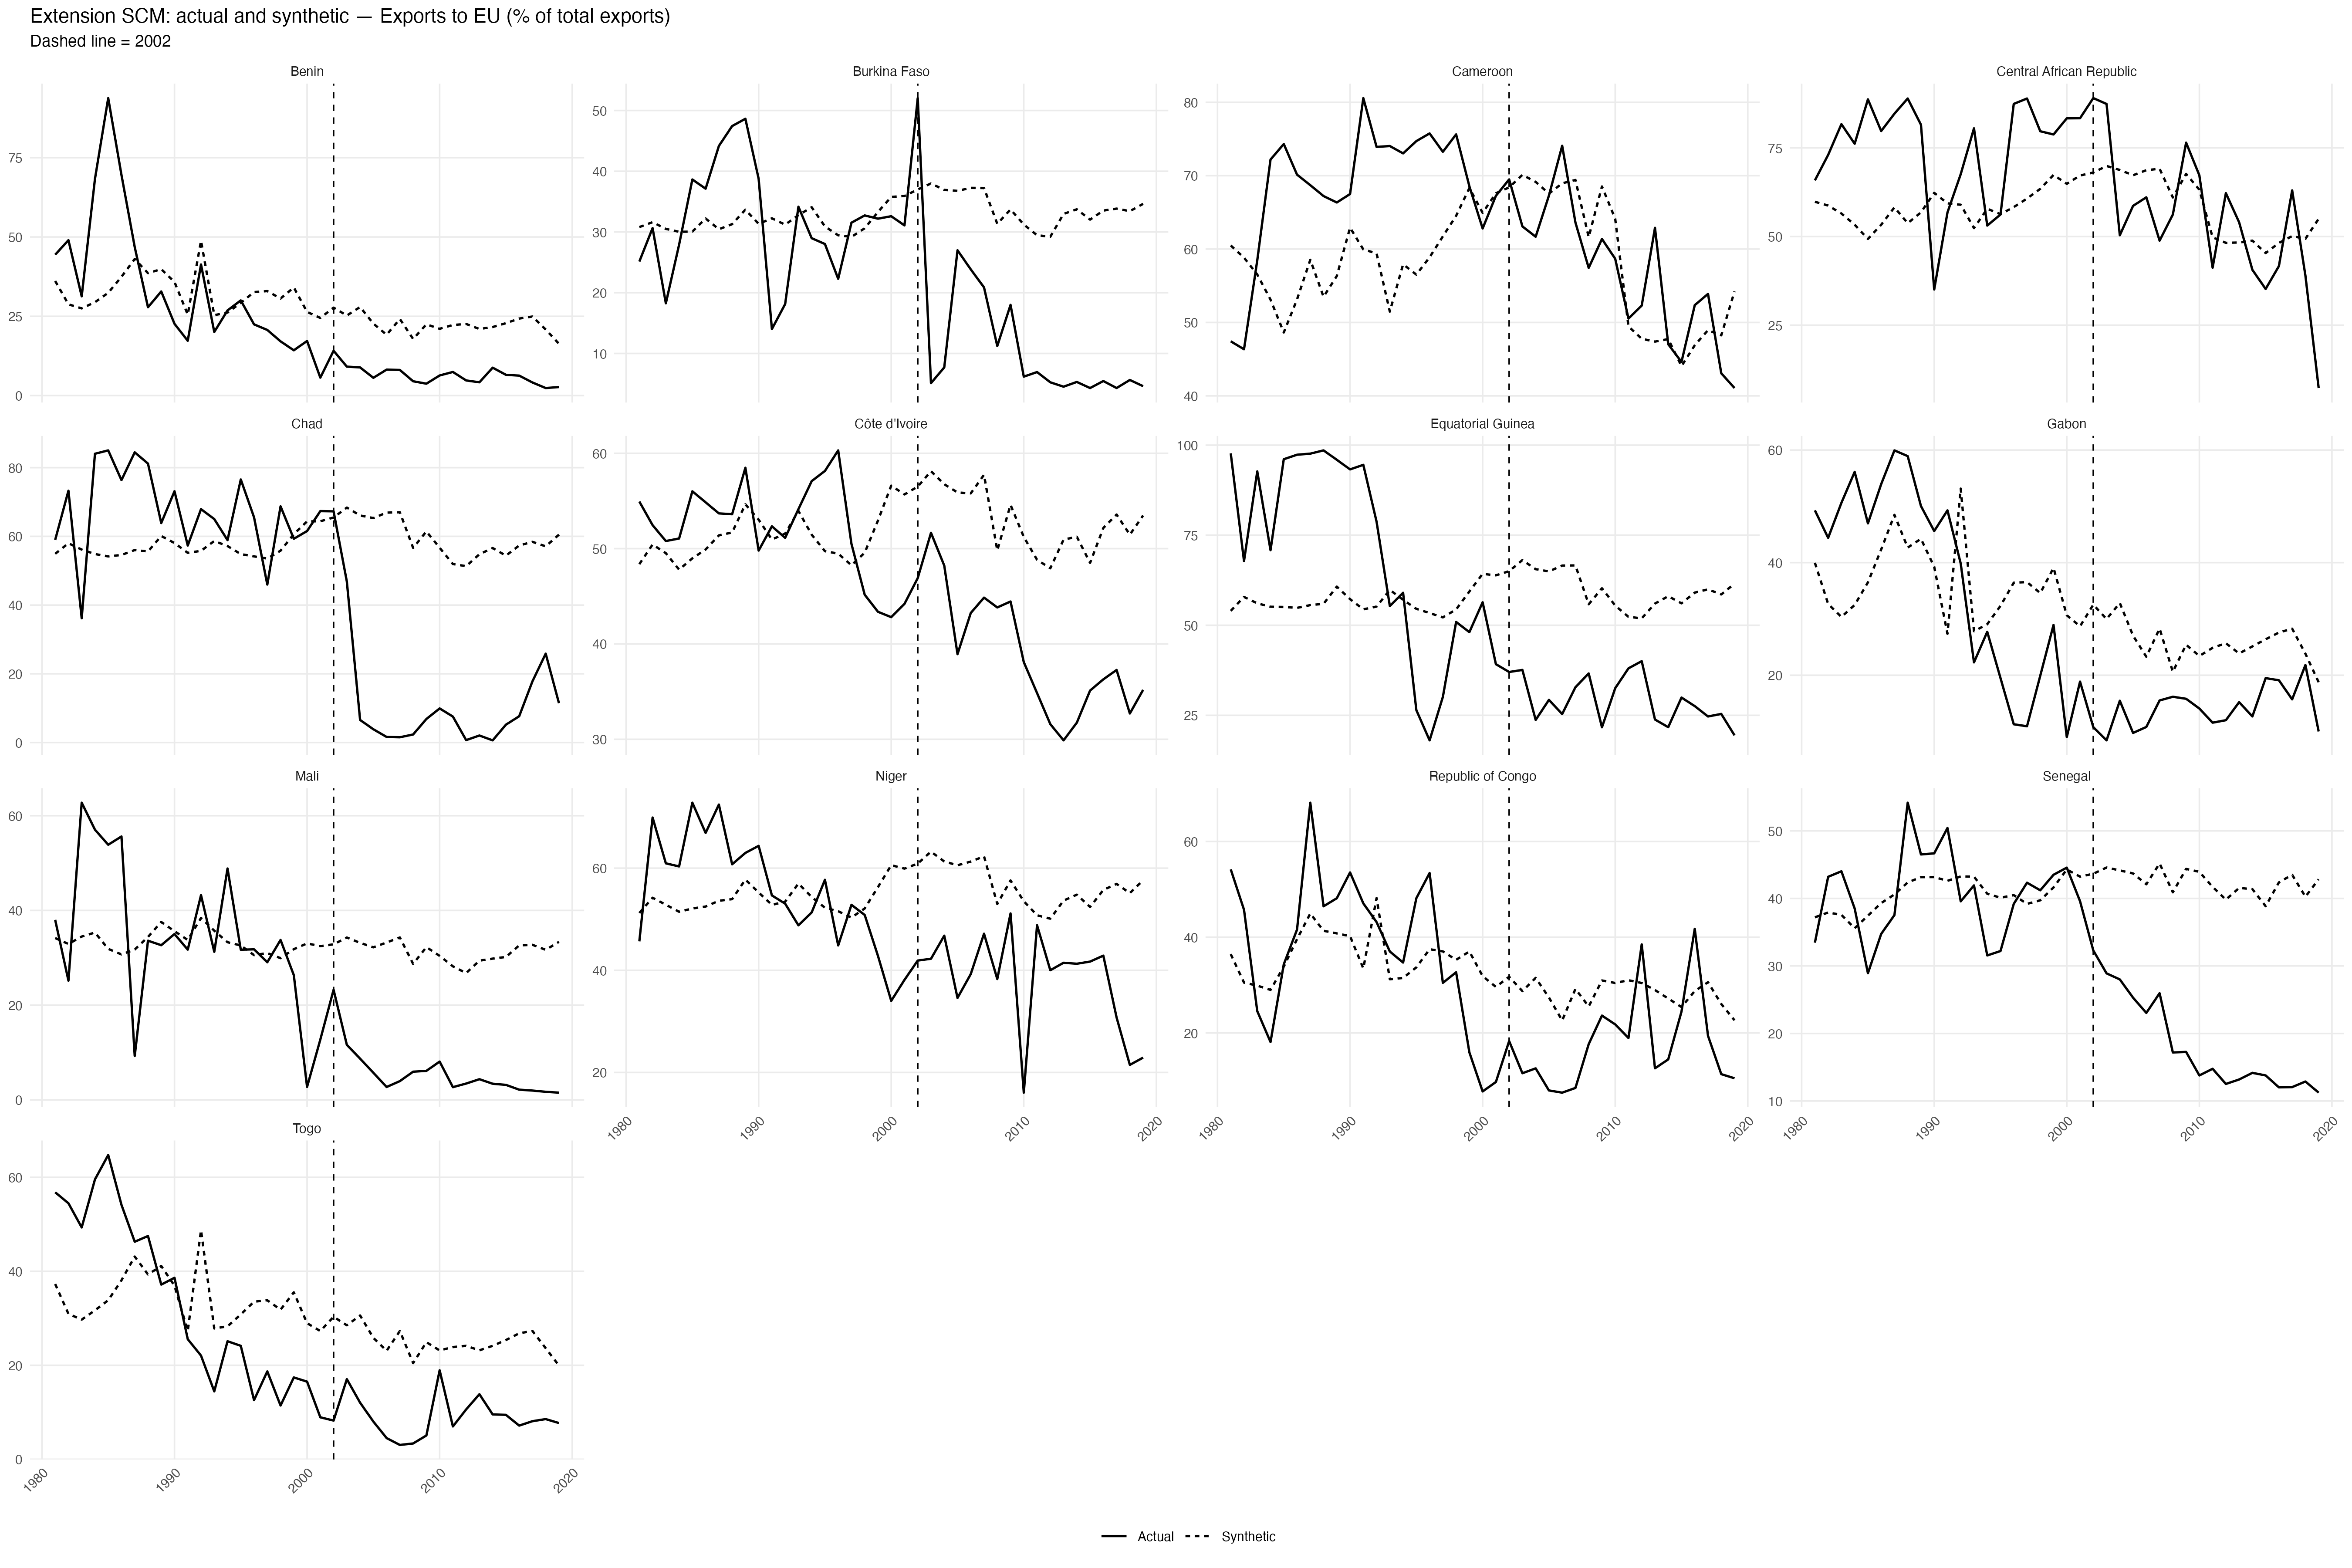
\includegraphics[width=\textwidth]{../output/extension_trade/figures/extension_trade_scm_paths_XEU.png}

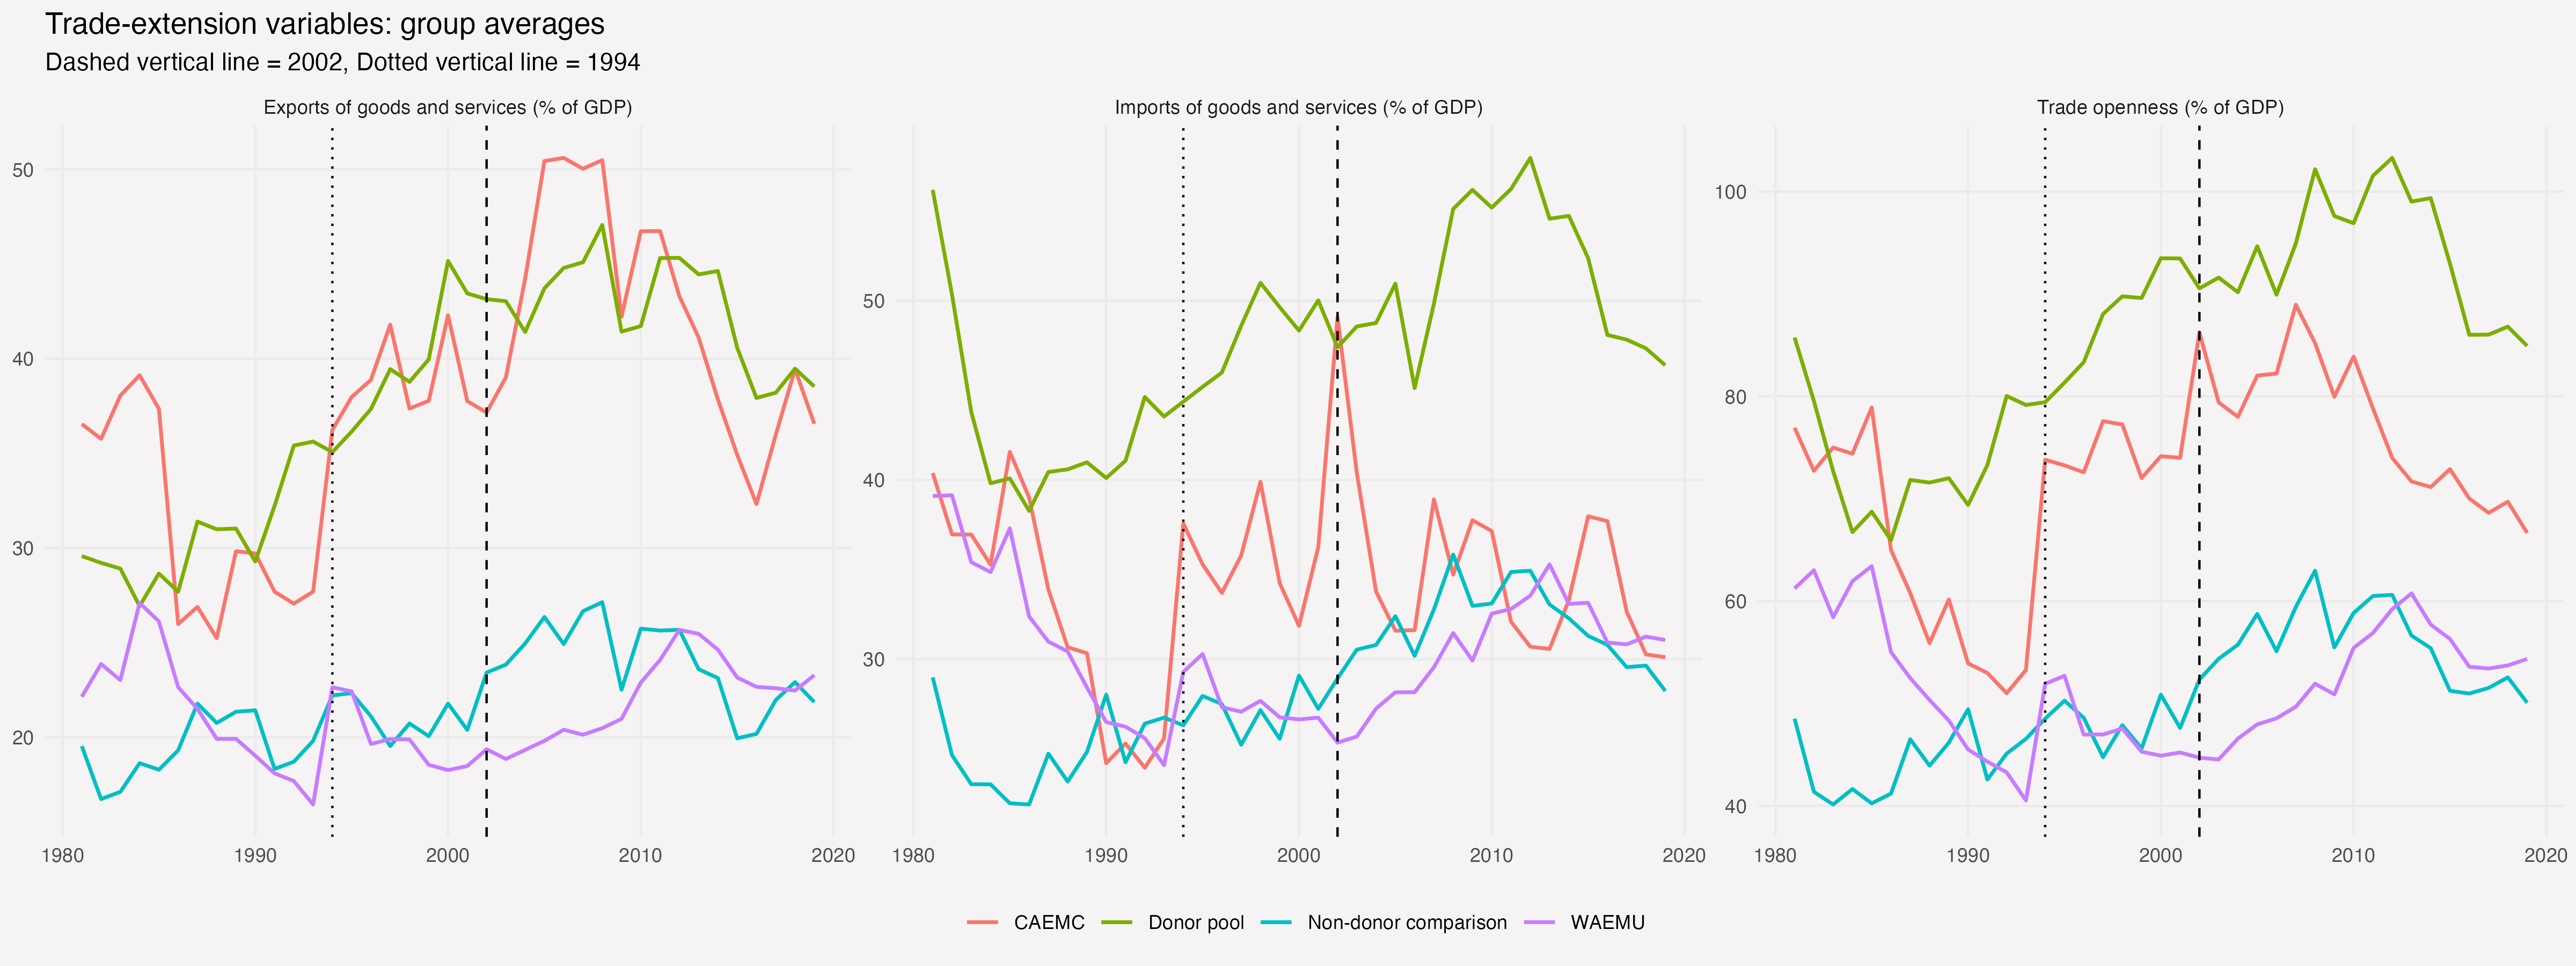
\includegraphics[width=\textwidth]{../output/extension_trade/figures/extension_trade_group_averages_reduced.png}

\section{Extension Placebo}

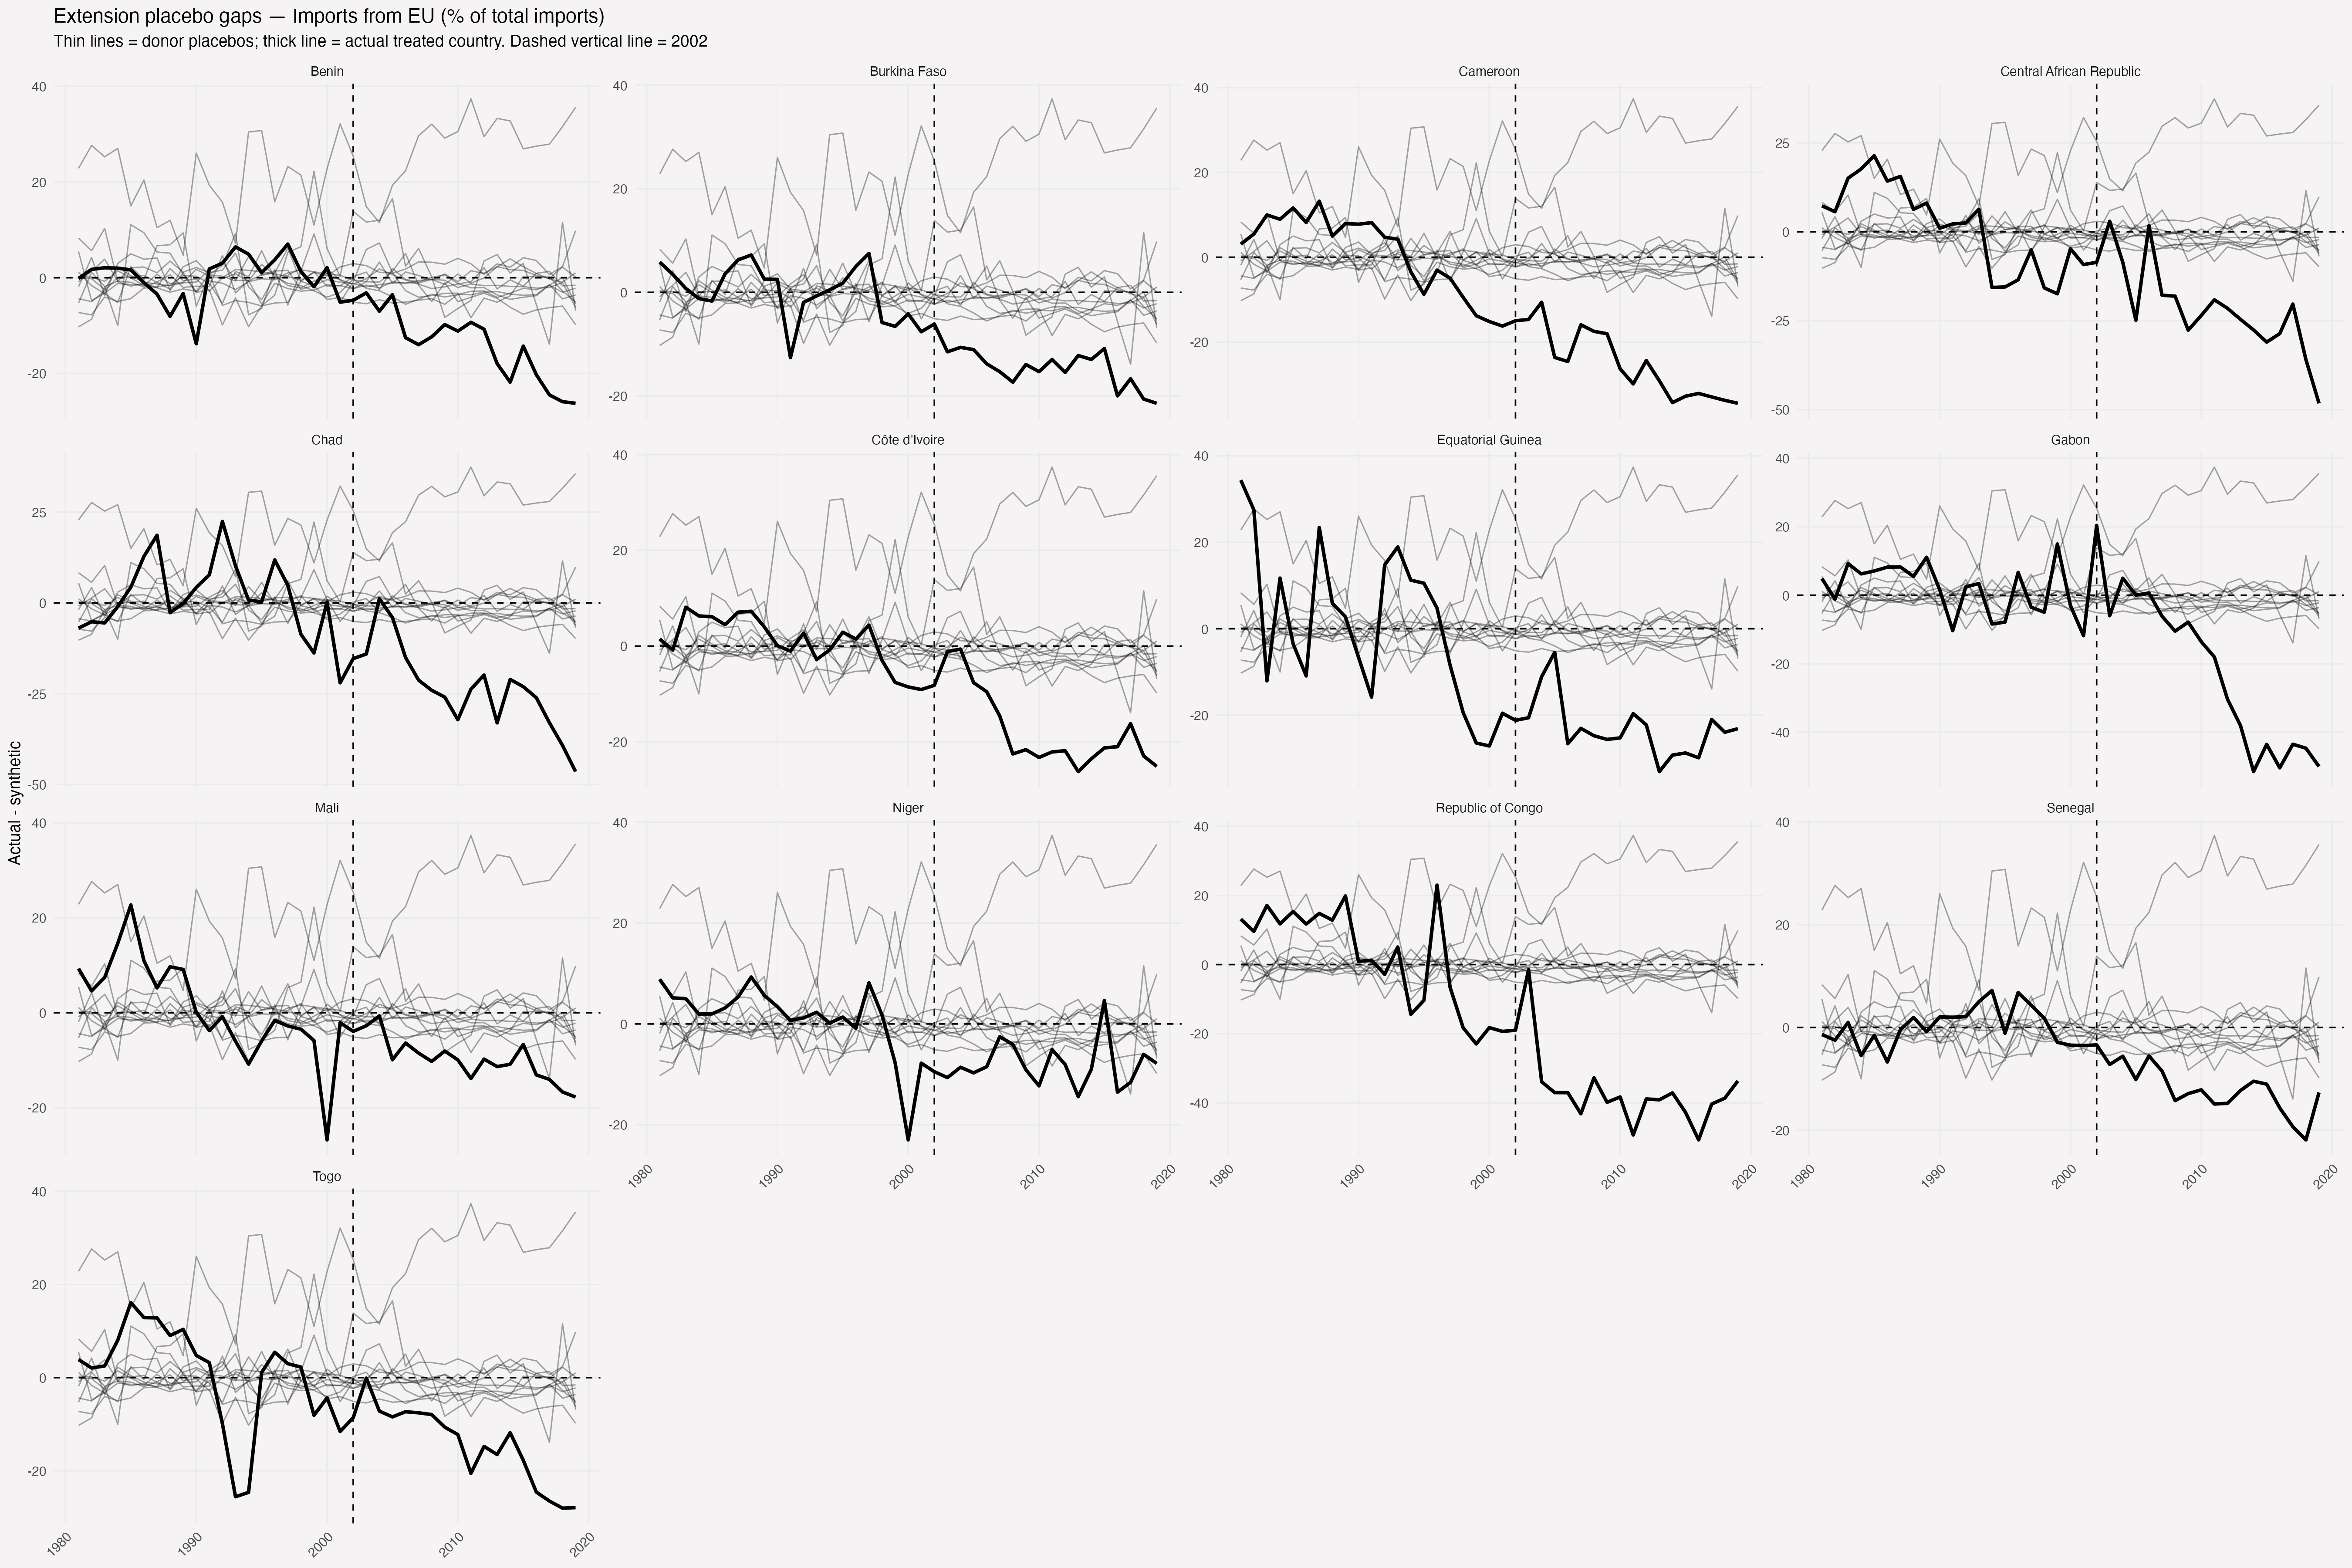
\includegraphics[width=\textwidth]{../output/extension_trade/placebo/figures/extension_trade_placebo_gaps_MEU.png}

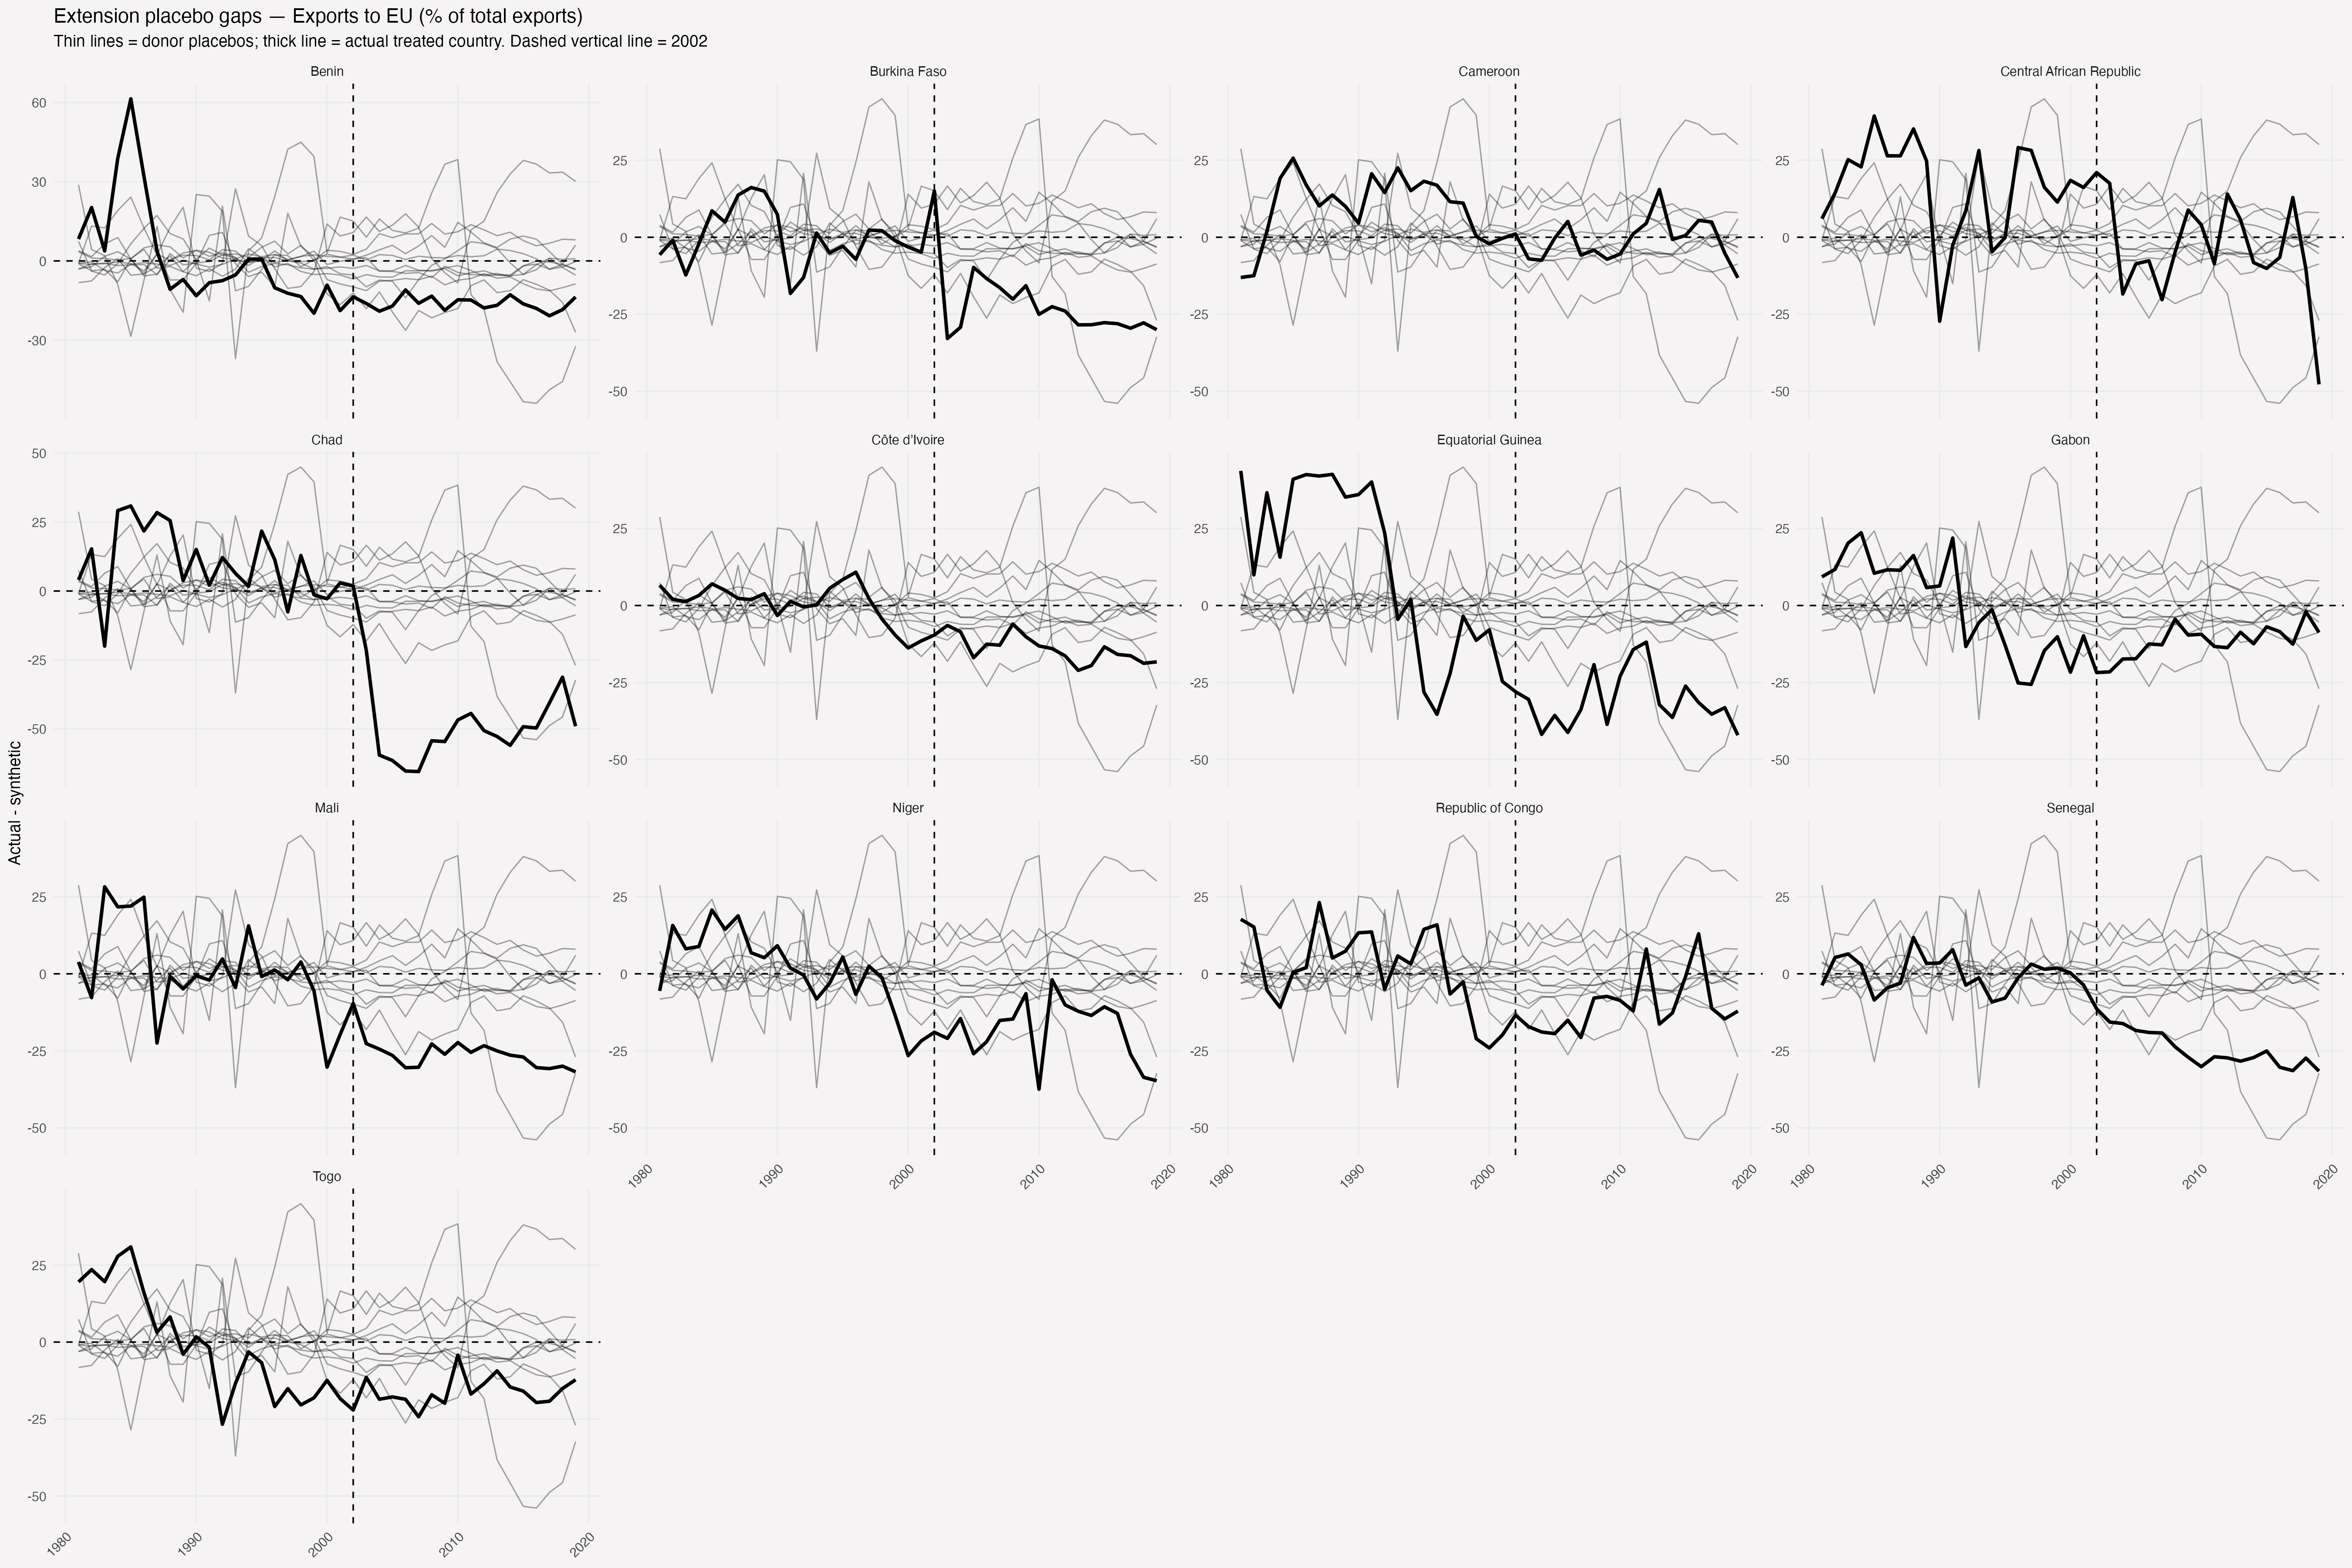
\includegraphics[width=\textwidth]{../output/extension_trade/placebo/figures/extension_trade_placebo_gaps_XEU.png}

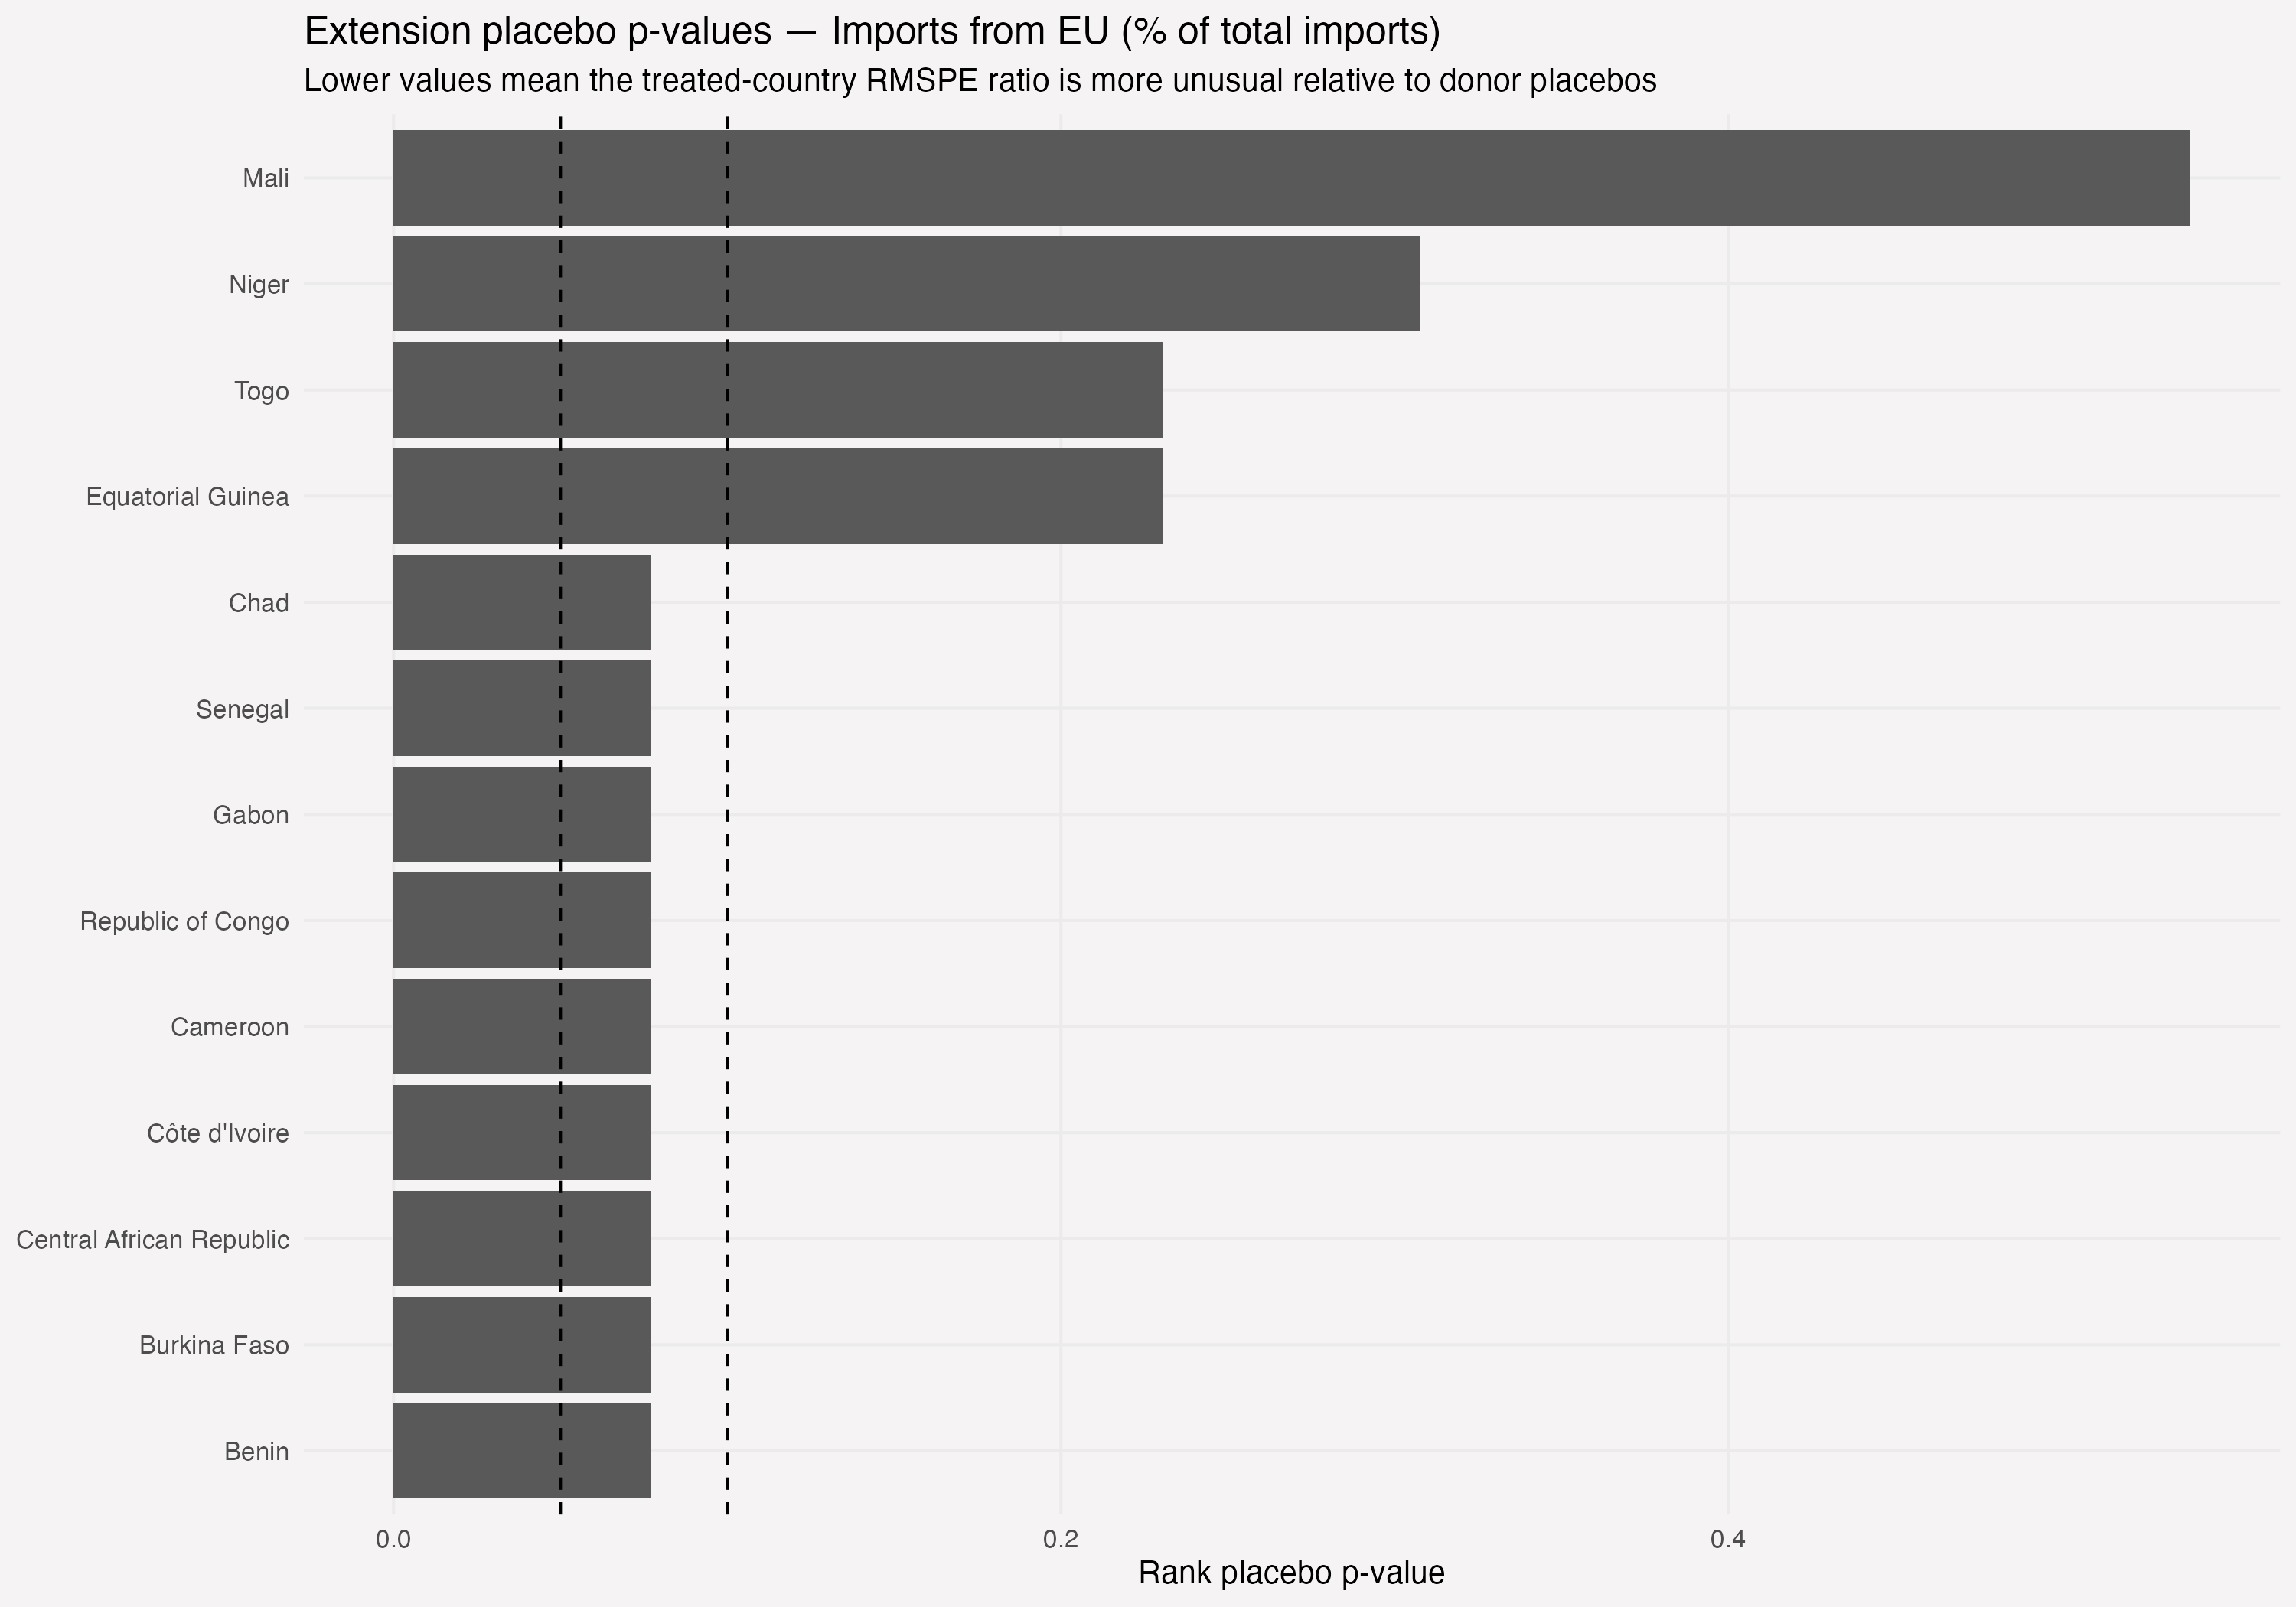
\includegraphics[width=\textwidth]{../output/extension_trade/placebo/figures/extension_trade_placebo_pvalues_MEU.png}

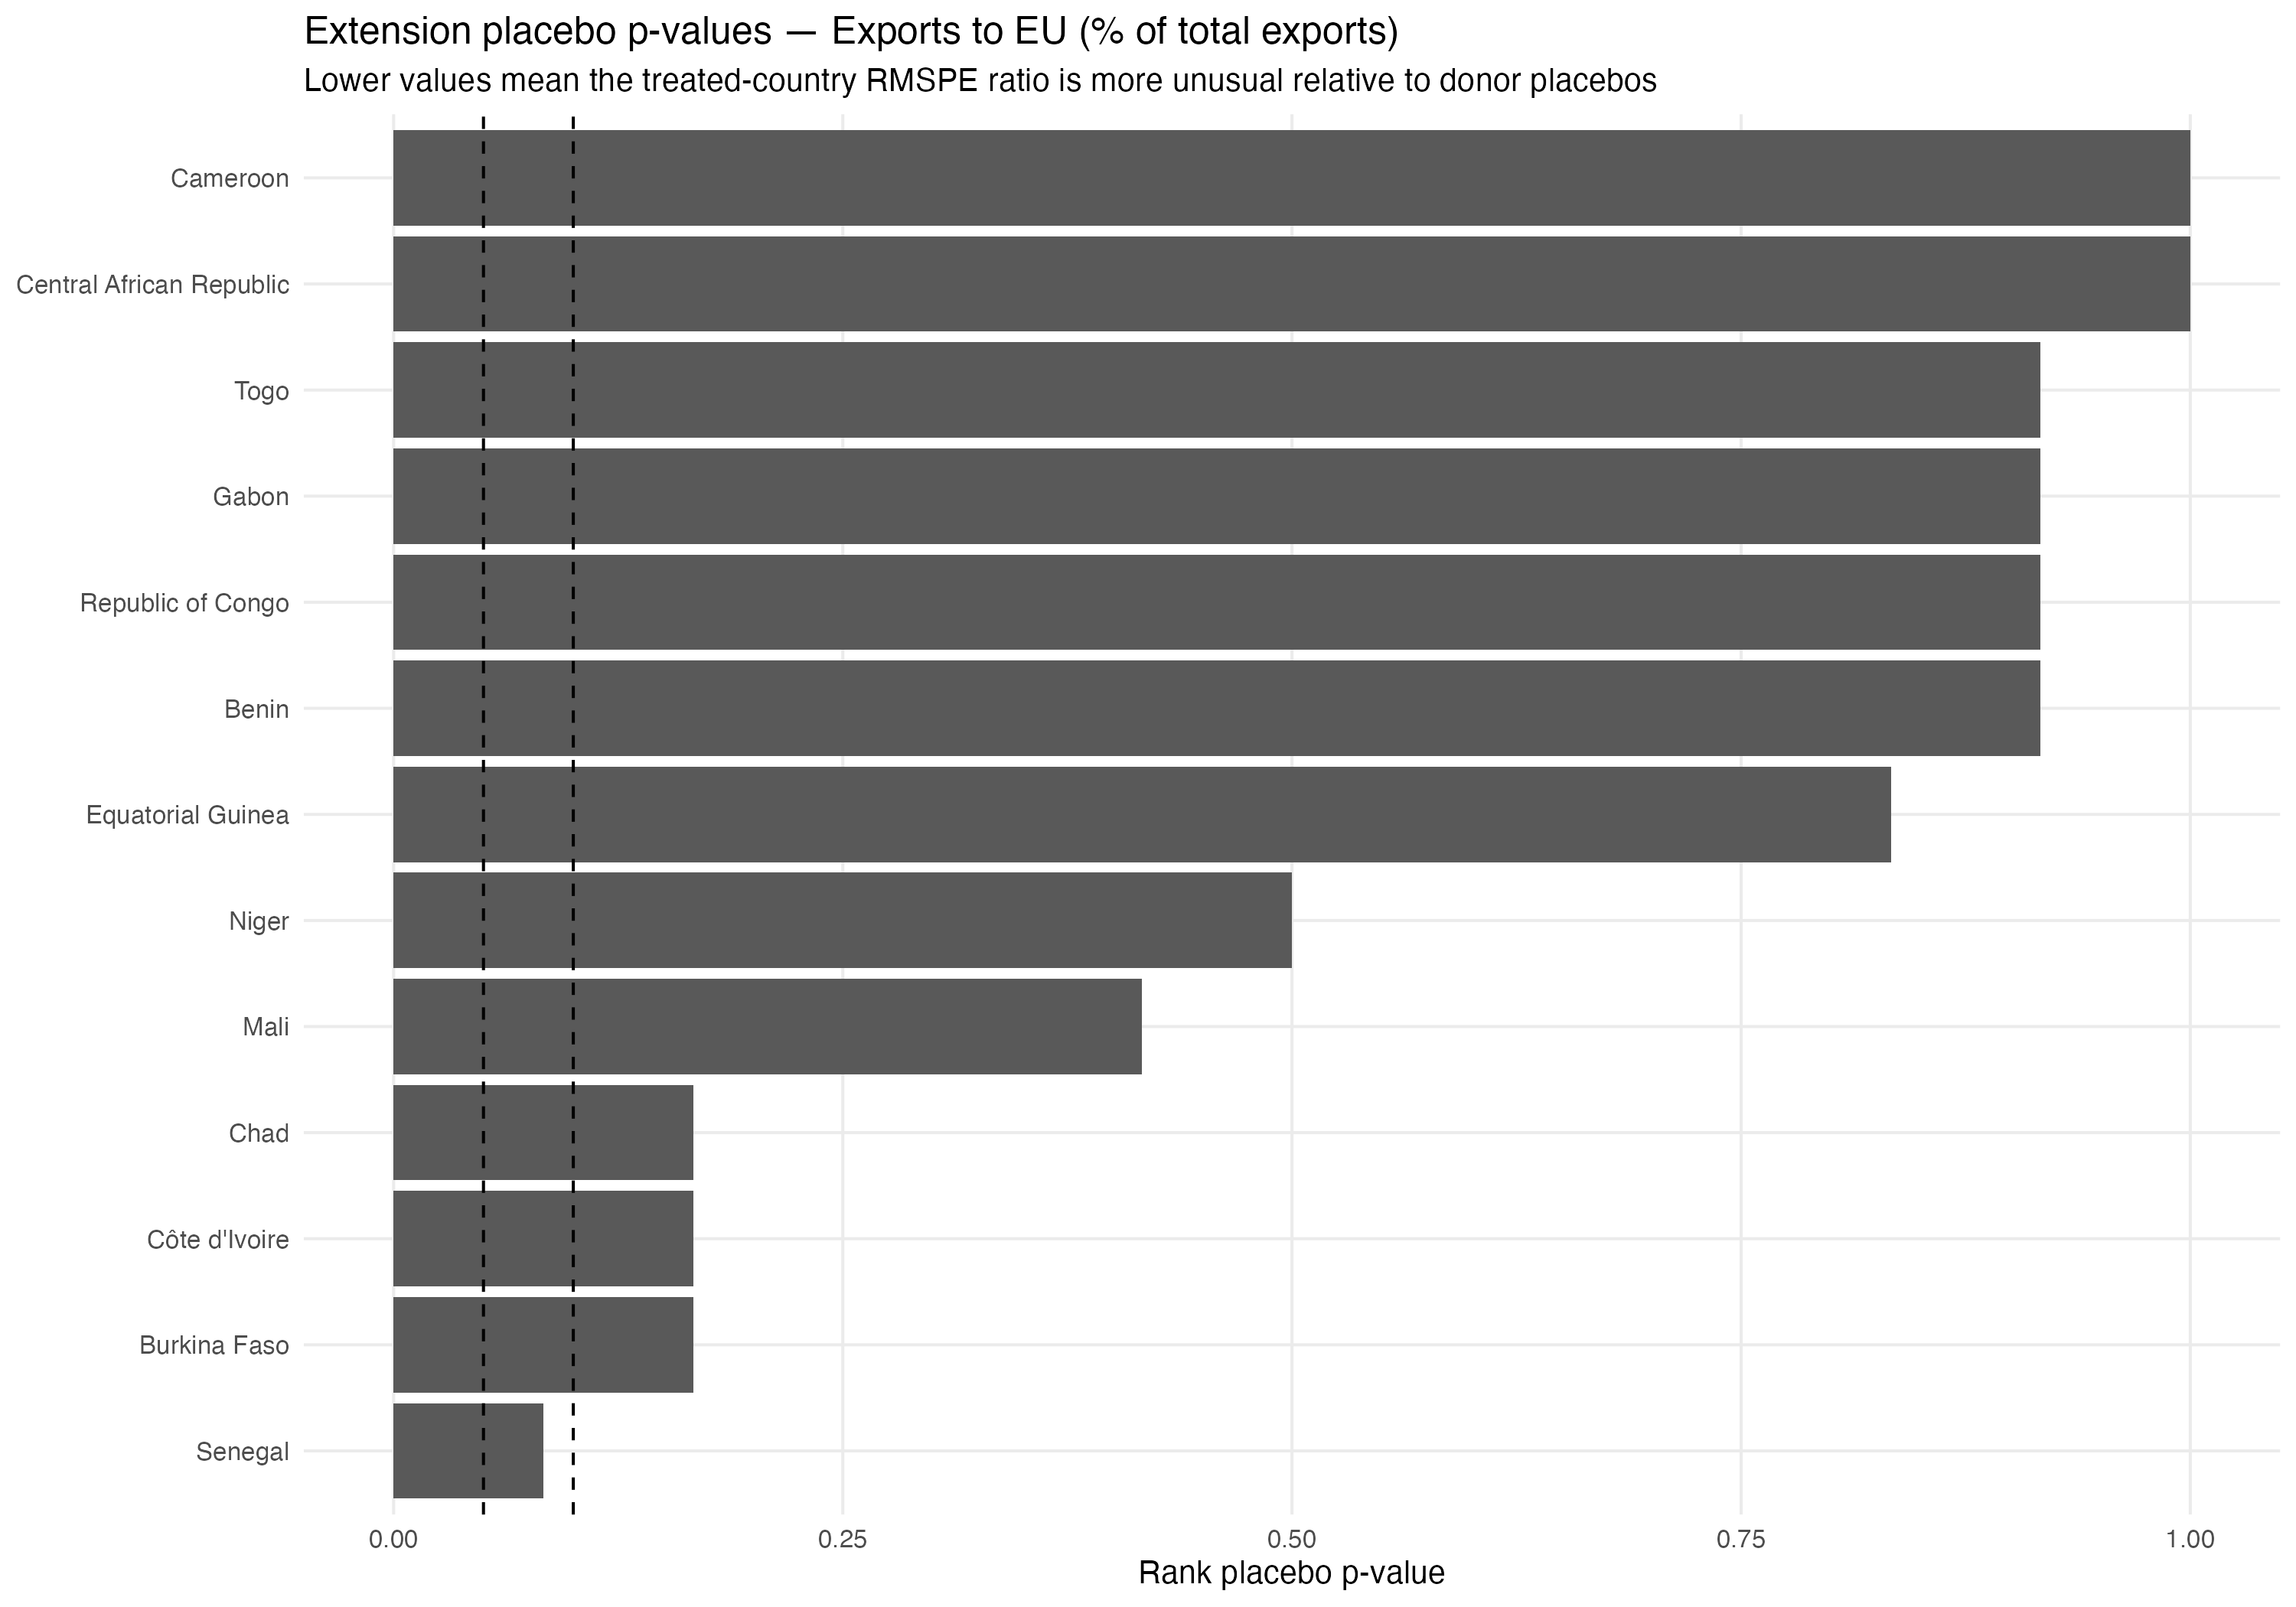
\includegraphics[width=\textwidth]{../output/extension_trade/placebo/figures/extension_trade_placebo_pvalues_XEU.png}

\section{Extension Placebo}


\end{document}